\documentclass[A4paper, british]{amsart}

%
% LOCAL FONT DEFINITIONS -- need to come first
%
%\usepackage{mathpazo}
\usepackage{libertine}
\usepackage[libertine]{newtxmath}

%
% STANDARD PREAMBLE
%
/home/pedro/git/templates/preamble.tex
\allowdisplaybreaks

%
% ABOUT FONT DEFINTIONS IN THE PREAMBLE
%
% Mathscr for sheaves use \sA, where A can be any letter. Exceptions and additions:
% % \E (vector bundles)
% % \F (coherent sheaves)
% % \G (coherent sheaves)
% % \hom (sheaf hom)
% % \I (ideal sheaves)
% % \L (line bundles)
% % \M (line bundles)
% % \O (structure sheaf)
% % \w (canonical sheaf)
%
% Mathcal use \calA. Exceptions and additions:
% % \U (open cover)
% % \X (families of varieties)
% % \Y (families of varieties)
%
% Mathbb use \bbA. Exceptions and additions:
% % \A (affine space)
% % \C (complex numbers)
% % \Gm (puctured affine line)
% % \k (field)
% % \N (natural numbers)
% % \P (projective space)
% % \Q (rational numbers)
% % \R (real numbers)
% % \V (geometric vector bundle)
% % \Z (integers)
%
% Boldfont for categories use \bfA. Additions:
% % \Coh (coherent sheaves)
% % \D (derived category)
% % \Db (bounded derived category)
% % \PSh (presheaves)
% % \QCoh (quasi-coherent sheaves)
% % \Sh (sheaves)
%
% Mathfrak for ideals
% % From \a to \e
% % \m and \n for maximal ideals

%
% THEOREM ENVIRONMENTS
%
% Theorems, propositions, etc (dark green)
\theoremstyle{darkgreentheorem}
\newtheorem{thm}{Theorem}[section]
\newtheorem{lm}[thm]{Lemma}
\newtheorem{prop}[thm]{Proposition}
\newtheorem{cor}[thm]{Corollary}
\newtheorem{conj}[thm]{Conjecture}
% Definitions (dark blue)
\theoremstyle{darkbluedefinition}
\newtheorem{defn}[thm]{Definition}
% Examples (dark red)
\theoremstyle{darkredexample}
\newtheorem{exa}[thm]{Example}
% Remarks (black)
\theoremstyle{remark}
\newtheorem{rem}[thm]{Remark}
\newtheorem{obs}[thm]{Observation}
\newtheorem{pbl}[thm]{Problem}
\newtheorem{fact}[thm]{Fact}
\newtheorem{q}[thm]{Question}
\newtheorem{nota}[thm]{Notation}
\newtheorem{exe}[thm]{Exercise}

%
% MATH OPERATORS
%
\DeclareMathOperator{\Hom}{Hom}
\DeclareMathOperator{\Ext}{Ext}
\DeclareMathOperator{\Fun}{Fun}
\DeclareMathOperator{\Cond}{Cond}
\DeclareMathOperator{\Ob}{Ob}
\DeclareMathOperator{\im}{im}
\DeclareMathOperator{\coker}{coker}
\let\Re\relax
\DeclareMathOperator{\Re}{Re}
\let\Im\relax
\DeclareMathOperator{\Im}{Im}
\DeclareMathOperator{\codim}{codim}
\DeclareMathOperator{\End}{End}
\DeclareMathOperator{\ext}{\E xt}
\DeclareMathOperator{\Sym}{Sym}
\DeclareMathOperator{\Hilb}{Hilb}
\DeclareMathOperator{\Spec}{Spec}
\DeclareMathOperator{\vol}{vol}
\DeclareMathOperator{\ord}{ord}
\DeclareMathOperator{\Supp}{Supp}
\DeclareMathOperator{\ihom}{\underline{Hom}}
\DeclareMathOperator{\iext}{\underline{Ext}}
\DeclareMathOperator{\GL}{GL}
\DeclareMathOperator{\Div}{Div}
\DeclareMathOperator{\Der}{Der}
\DeclareMathOperator{\rk}{rk}
\DeclareMathOperator{\Aut}{Aut}
\DeclareMathOperator{\Exc}{Exc}
\DeclareMathOperator{\Hess}{Hess}

%
% OTHER COMMANDS
%
% Additional categories
\newcommand{\CHaus}{\mathbf{CHaus}}
\newcommand{\ED}{\mathbf{ED}}
\newcommand{\HH}{HH}
\newcommand{\CG}{\mathbf{CG}}
\newcommand{\Solid}{\mathbf{Solid}}
% Uncategorized
\newcommand{\CP}{\mathbb{CP}}
\renewcommand{\H}{\mathcal{H}}
\newcommand{\cbbD}{\bar{\mathbb{D}}}
\newcommand{\1}{\mathbbm{1}}
\newcommand{\pe}{*_{proét}}
\renewcommand{\u}[1]{\underline{#1}}
\newcommand{\ot}{\otimes}
\newcommand{\op}{\oplus}
\newcommand{\fp}[1]{\times_{#1}}
\newcommand{\id}{\mathrm{id}}
\newcommand{\ev}{\mathrm{ev}}
\newcommand{\grd}{^{\bullet}}
\newcommand{\prp}{^{\perp}}
\newcommand{\dual}{^{\vee}}
\newcommand{\db}{\marginnote{\dbend}}
\newcommand{\tms}{\times}
\newcommand{\sub}{\subseteq}
\newcommand{\epi}{\twoheadrightarrow}
\newcommand{\mono}{\hookrightarrow}
\newcommand{\LCA}{\mathrm{LCA}}
\newcommand{\solid}{^{\blacksquare}}
\newcommand{\dsolid}{^{L\blacksquare}}
\newcommand{\usolid}{_{\blacksquare}}

%
% AUTHOR INFO
%
\author{Pedro Núñez}

%
% CONTENT DETAILS
%
\title[Various lecture notes]{Various lecture notes}
\date{\today}

%
% LINKS AND PDF OPTIONS
%
\makeatletter
\hypersetup{
  pdfauthor={\authors},
  pdftitle={\@title},
  pdfstartview={Fit},
  pdfpagelayout={TwoColumnRight},
  pdfpagemode={UseOutlines},
  bookmarks,
  colorlinks,
  linkcolor=linkblue,
  citecolor=linkred,
  urlcolor=linkred}
\makeatother

\begin{document}

\maketitle

\tableofcontents

\section{About these notes}

The purpose of these notes is to keep the material seen in lectures a bit organized and easily accesible from one single place, but they don't intend to be complete and they will surely be full of typos and mistakes\footnote{If you find any, please let me know! You can do this from \href{https://github.com/pedro-nlb/notes}{GitHub} or more directly with an email at \href{mailto:pedro.nunez@math.uni-freiburg.de}{pedro.nunez@math.uni-freiburg.de}}.

Warnings will be marked with a \href{https://en.wikipedia.org/wiki/Bourbaki_dangerous_bend_symbol}{dangerous bend} symbol on the margin \db.

\section{[CM] Talk 1 (Johan) - Condensed Sets - 21.10.19}

\subsection{Introduction}

One of the main motivations for condensed mathematics is that topological algebraic objects have usually poor categorical and functorial properties.
For instance, topological abelian groups do not form an abelian category:

\begin{exa}
    $\R_{disc}\to \R$ is epi and mono, but not iso.
\end{exa}

Another motivation is coherent duality:

\begin{thm}
    Let $f\colon X\to Y$ be a proper or quasi-projective morphism of Noetherian schemes of finite Krull dimension. Then there exists a right adjoint $f^{!}$ to the derived direct image functor $f_{!}=Rf_{*}\colon \Db(\QCoh(X))\to \Db(\QCoh(Y))$.
\end{thm}

At some point analytic rings will come up.
We will then look at the category of solid modules, in which the 6-functor formalism works nicer than in the classical setting (e.g. when $f_{!}$ is not defined in the classical setting, $f_{!}$ takes non-discrete values in the condensed settings, which are "not there" in the classical setting).

\begin{defn}
    Pro\'{e}tale site of a point, denoted $\pe$, is the category of profinite sets with finite jointly surjective families of continuous maps as covers.
    A \textit{condensed set} (resp. group, ring, ...) is a sheaf of sets (resp. groups, rings, ...) on $\pe$.
    We denote by $\Cond(\bfC)$ the category of condensed objects of a category $\bfC$.
\end{defn}

\begin{defn}
    A \textit{condensed set} (resp. group, ring, ...) is a contravariant functor $X$ from $\pe$ to the category of sets (resp. groups, rings, ...) such that 
    \begin{enumerate}[label=\roman*)]
	\item $X(\varnothing)=*$.
	\item For all profinite sets $S_{1}$ and $S_{2}$ the natural map
	    \[ X(S_{1}\sqcup S_{2})\to X(S_{1})\times X(S_{2}) \]
	    is an isomorphism.
	\item For any surjection of profinite sets $f\colon S'\twoheadrightarrow S$ we get an induced\footnote{Since the pullback diagram is commutative, the image of $X(f)$ is indeed induces a morphism as claimed.} isomorphism
	    \[ X(S)\to \{ x\in X(S')\mid \pi_{1}^{*}(x)=\pi_{2}^{*}(x)\in X(S'\fp{S}S')\} \]
    \end{enumerate}
\end{defn}

We will call $X(*)$ the \textit{underlying object} in $\bfC$ of a condensed object.

\begin{rem}
    We will use $T$ for topological spaces vs. $X,Y$ for condensed sets, as opposed to Scholze's mixing of those notations.
\end{rem}

\subsection{Recollections on sheaves on sites}

Let $F$ be a presheaf on a site, which is just a contravariant functor to whatever category in which our sheaves are gonna take values.
If $U=\cup_{i}U_{i}$ is an open cover, the topological sheaf axiom could be phrased as: $F(U)$ is an equalizer of the diagram
\[ \prod_{i}F(u_{i})\rightrightarrows \prod_{i,j}F(U_{i}\cap U_{j}). \]
Note that $U_{i}\cap U_{j}$ is just the fiber product of the two inclusions.

\begin{defn}[Coverage]
    See definition 2.1 in \href{https://ncatlab.org/nlab/show/coverage}{nCat}.
\end{defn}

\begin{defn}
    $F$ a presheaf on $\bfC$.
    A collection $(s_{i})\in \prod_{i}F(U_{i})$ for $\{f_{i}\colon U_{i}\to U\}$ a covering is called a \textit{matching family} if for all $h\colon V\to U$ we have $g^{*}(s_{i})=h^{*}(s_{j})$ for $g$ and $h$ in the diagram
    \begin{center}
	\begin{tikzcd}
	    V\arrow{r}{h}\arrow{d}{g} & U_{j}\arrow{d}{f_{j}} \\
	    U_{i}\arrow{r}{f_{i}} & U
	\end{tikzcd}
    \end{center}
\end{defn}

\begin{defn}
    $F$ is a sheaf with respect to $\{U_{i}\to U\}$ if for all matching families $(s_{i})$ there exists a unique $s\in F(U)$ such that $f_{i}^{*}(s)=s_{i}$.
    We say that $F$ is a \textit{sheaf} if it is a sheaf for all covering families.
\end{defn}

\begin{rem}
    A sheaf of abelian groups is just a commutative group object in the category of sheaves of sets.
\end{rem}

\begin{thm}
    If $\bfC$ is a site, then $\Ab(\bfC)$ is an abelian category.
\end{thm}

\begin{defn}
    An additive category is a category in which the hom-sets are endowed with an abelian group structure in a way that makes composition bilinear and such that finite biproducts exist.
\end{defn}

Recall Grothendieck's axioms:
AB1) Every morphism has a kernel and a cokernel.
AB2) For every $f\colon A\to B$, the natural map $\operatorname{coim}(f)\to \im{f}$ is an iso.
AB3) All colimit exist.
AB4) AB3) + arbitrary direct sums are exact.
AB5) AB3) + arbitrary filtered colimits are exact.
AB6) AB3) + $J$ an index set, $\forall j\in J$ a filtered category (think of directed set) $I_{j}$, functors $M\colon I_{j}\to \bfC$, then
\[\varinjlim_{(i_{j}\in I_{j})_{j}}\prod_{j} M_{i_{j}}\to \prod_{j\in J}\varinjlim_{i_{j}\in I_{j}} M_{i_{j}} \]

\begin{thm}
    $\bfC$ a site. Then $\Ab(\bfC)$ satisfies AB3), AB4), AB5) and AB6).
\end{thm}

In fact, our case is even nicer:

\begin{thm}
    $\Cond(\Ab)$ in addition satisfies AB6) and AB4*).
\end{thm}

\subsection{Compactly generated topological spaces}

\begin{defn}
    A topological space $T$ is called \textit{compactly generated} if any function $f\colon T\to T'$ is continuous as soon as the composite $S\to T\to T'$ is continuous for all maps $S\to T$ where $S$ is compact and Hausdorff.
    See also \href{https://ncatlab.org/nlab/show/compactly+generated+topological+space}{nCat}.
\end{defn}

The inclusion functor $\CG \hookrightarrow \Top$ has a right adjoint $(-)^{cg}$.
If $T$ is any topological space, then the topology on $T^{cg}$ is the finest topology on $T$ such that $\sqcup_{S\to T}S\to T$ is continuous, where $S$ ranges over all compact Hausdorff spaces.

Let $T$ be a topological space.
We view $T$ as a presheaf on $\pe$ by setting $T(S)=\Hom_{\Top}(S,T)$ for all profinite sets $S$.
We denote this by $\u{T}$.
Claim: $\u{T}$ is a sheaf.
\begin{enumerate}[label=\roman*)]
    \item The first condition $\u{T}(\varnothing)=*$ is true, because there is exactly one morphism from the empty set to any topological space.
    \item $\u{T}(S_{1}\sqcup S_{2})=\u{T}(S_{1})\times \u{T}(S_{2})$ by universal property of disjoint union.
    \item For any surjection $S'\twoheadrightarrow S$ we get an isomorphism
	\[ \u{T}(S)\to \{ x\in \u{T}(S')\mid \pi_{1}^{*}(x)=\pi_{2}^{*}(x)\in \u{T}(S'\fp{S}S')\}\]
\end{enumerate}

Since $\Top\to \Cond(\Set)$ preserves products, group objects are preserved, so it maps topological groups to condensed groups etc.

\begin{prop}
    \begin{enumerate}[label=\roman*)]
	\item This functor is faithful and fully faithful when restricted to the full subcategory of compactly generated spaces.
	\item It admits a left adjoint $X\mapsto X(*)_{top}$ where $X(*)_{top}$ gets the quotient topology of $\sqcup_{S\to X}S\to X(*)$ as above.
	    The counit $I(*)_{top}\to T$ agrees with $T^{cg}\to T$.
    \end{enumerate}
\end{prop}

Coming back to our original example:

\begin{exa}
    $\mathbb{R}_{disc}\to \mathbb{R}$ can be seen in the condensed world as $\u{\mathbb{R}_{disc}}\to \u{\mathbb{R}}$, i.e. from locally constant functions to continuous functions.
    This is still a mono, but now it is not an epi.
    The cokernel $Q$ can be described as $Q(S)=\{ S\to \mathbb{R}\text{ continuous }\}/\{ S\to \mathbb{R}\text{ locally constant }\}$.
    Note in particular that the underlying set of $Q$ is just $*$, reflecting the fact that the cokernel was trivial in the classical setting.
\end{exa}

\section{[LT] Lecture 1 - 22.10.19}

\subsection{Introduction and overview of the course}

An \textit{algebraic variety} is the solution set of a family of polynomial equations in $\C^{n}$.
For example, if $f(x,y,z,t)=xy-tz$, then
\[ V(f)=\{(x,y,z,t)\in \C^{4}\mid xy-tz=0\} \]
is an algebraic variety in $\C^{4}$.
Another example would be the parabola $\{ y-x^{2}=0\}\subseteq \C^{2}$.

Let us focus on $V(f)$ and set $t=1$.
Then $X=V(f)\cap \{ t=1 \}=\{(x,y,z)\in \C^{3}\mid xy=z\}$ can be seen as a family of complex curves parametrized by the variable $z$.
For $z=0$, the complex curve $X_{0}$ has an \textit{ordinary double point} at the origin:

\begin{figure}[h]
    \centering
    \includegraphics[scale=.5]{odpfiber}
    \caption{Topological picture of our ODP.}
    \label{fig:odpfibre}
\end{figure}

Singularities arise naturally while studying the topology of algebraic varieties, and ODP's are a particularly nice kind of singularities.

For $z\neq 0$ we get an equation which looks like $xy=1$.
In this case we have the following picture:

\begin{figure}[h]
    \centering
    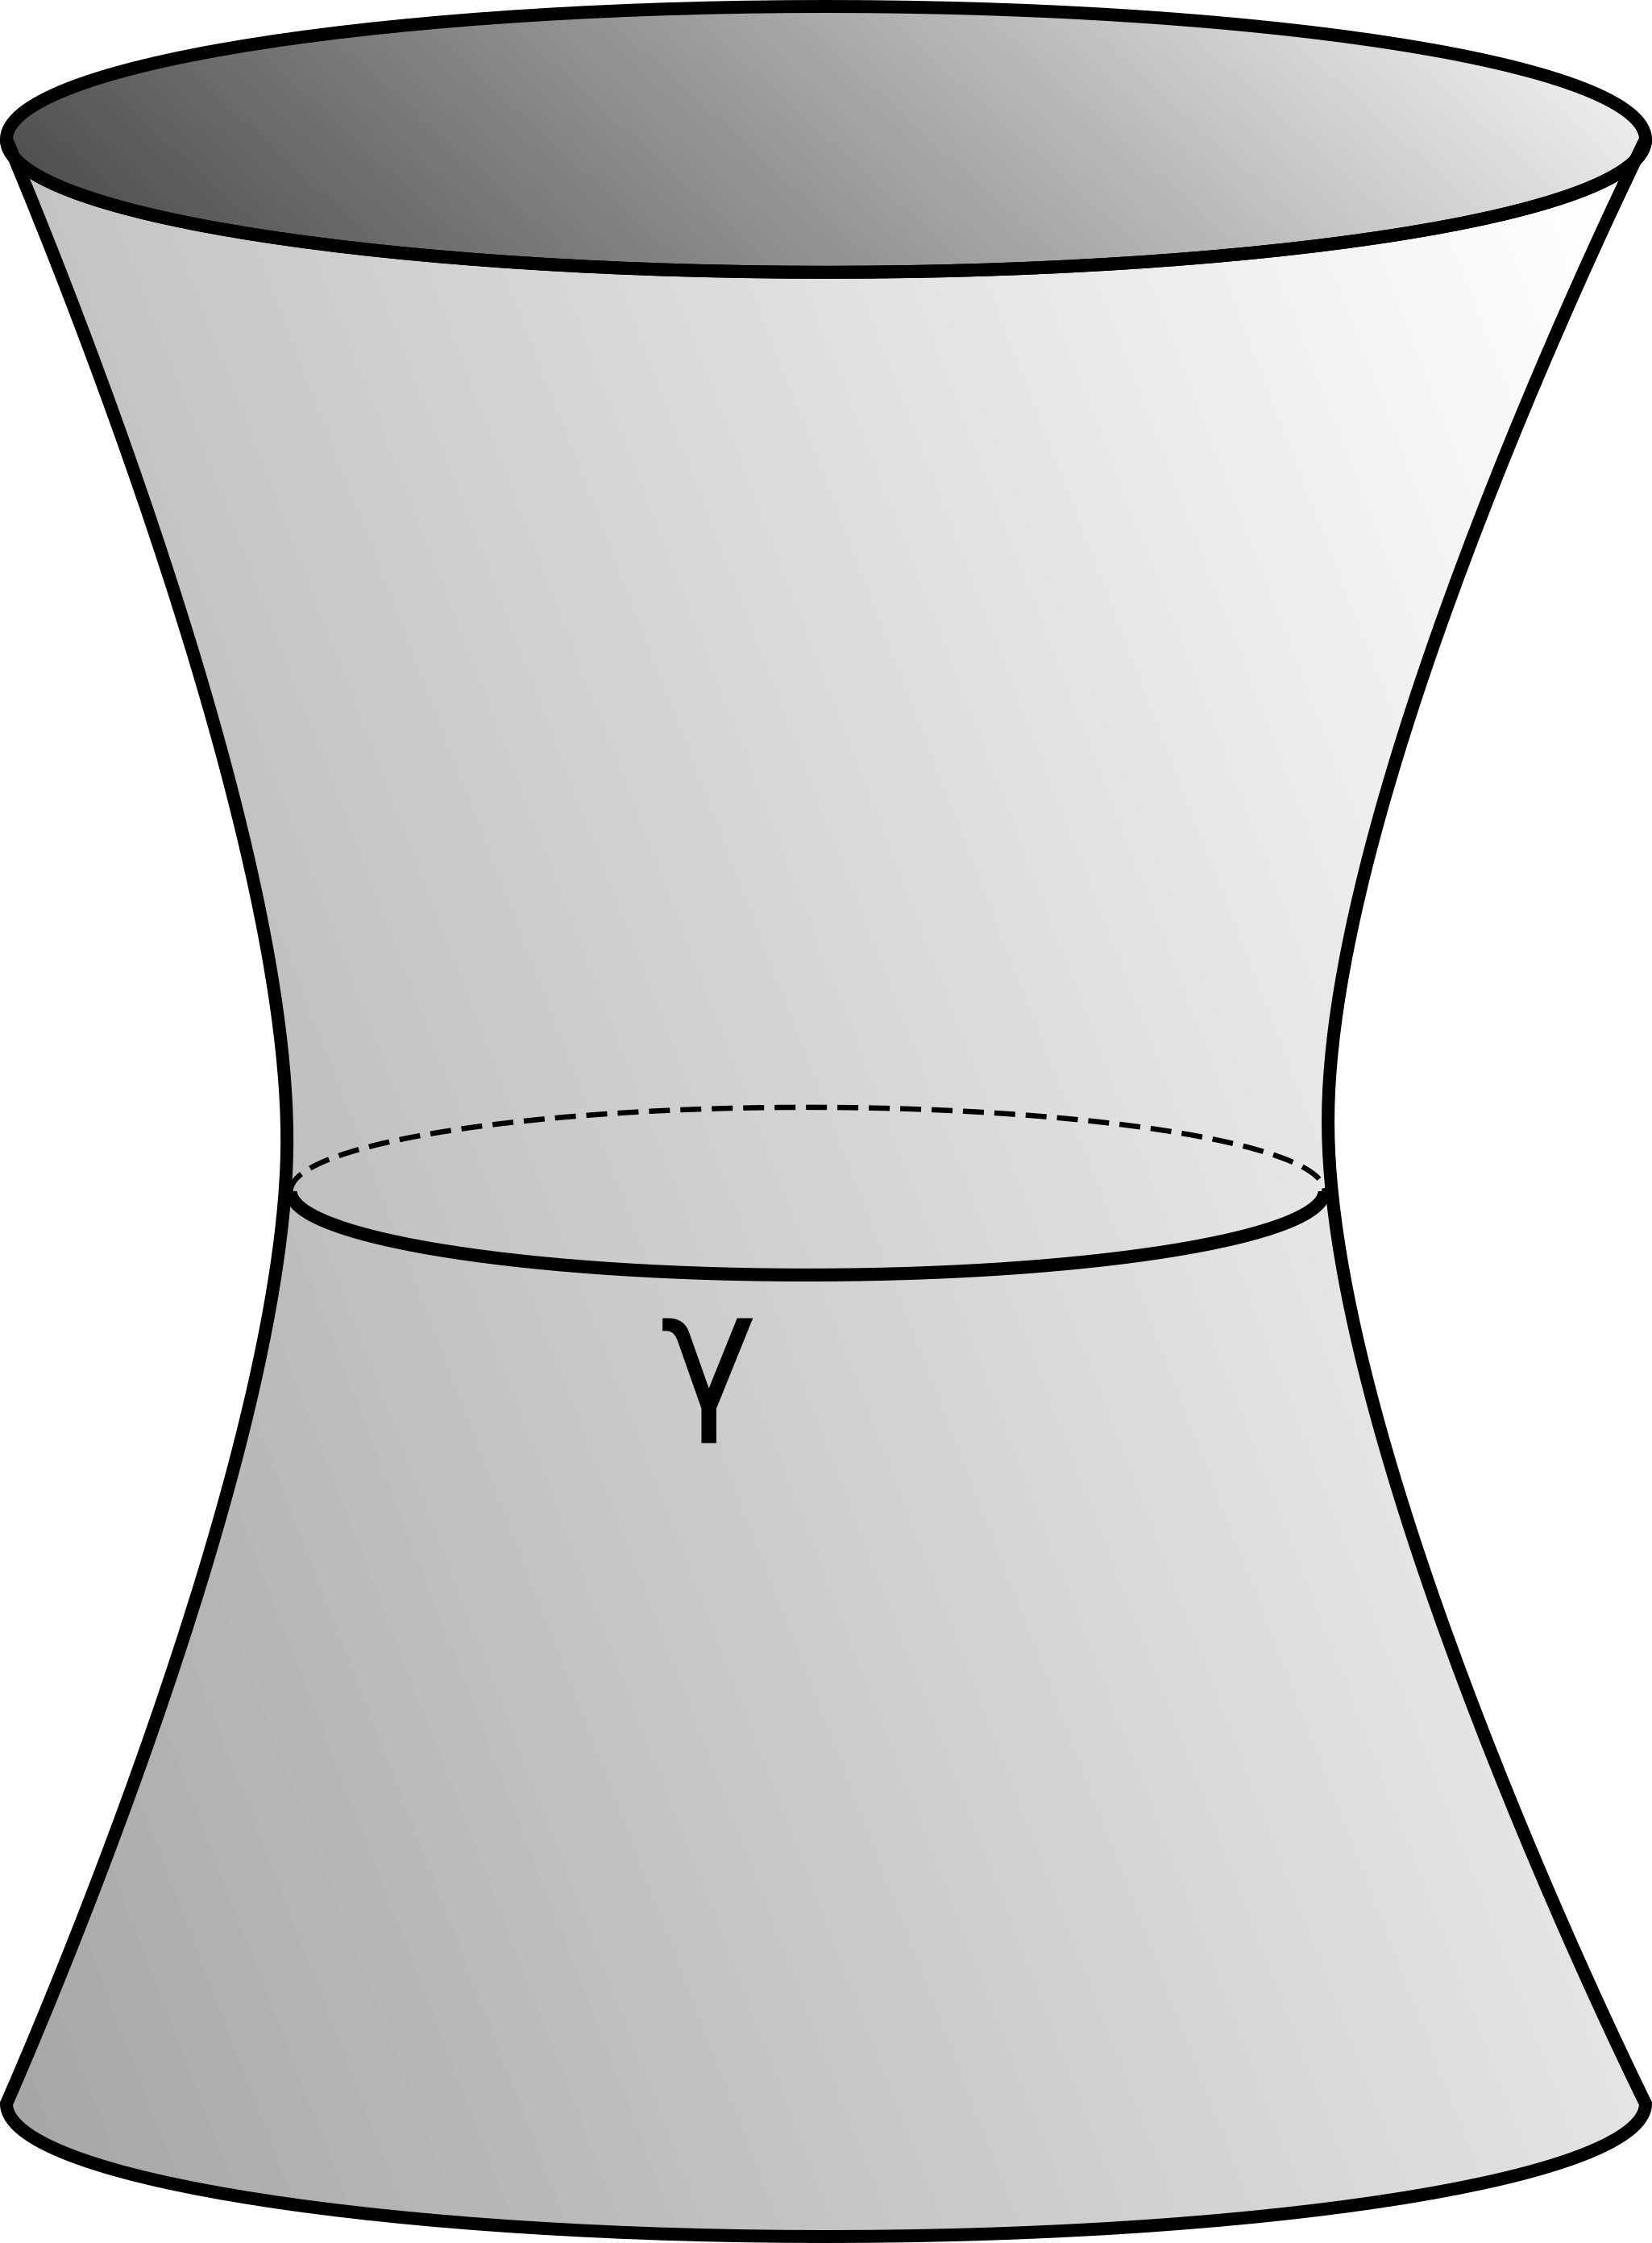
\includegraphics[scale=.8]{smoothfiber}
    \caption{Topological picture of $X_{z}$.}
    \label{fig:smoothfibre}
\end{figure}

As $z\to 0$, the central loop $\gamma$ contracts to the ordinary double point.
Note in particular that $X_{0}$ has trivial fundamental group (hence trivial $1$-homology), whereas $X_{z}$ does not.

We have a projection $\pi\colon X\to \C$, and Ehresmann's lemma tells us that for all disks $D\subseteq \C$ not containing $0$ we have $\pi^{-1}(D)\cong D\times X_{z_{0}}$ for any $z_{0}\in D$.

\begin{q}
    Given an arbitrary nonsingular algebraic variety $X\subseteq \C^{n}$, can we find a map $\pi\colon X\to \C$ such that the fibers $X_{t}$ are nonsingular for all but finitely many $t\in \C$ and such that the singular fibres have at worst ODP singularities?
\end{q}

Notice how we are missing information at infinity, e.g. $y=x^{2}$ versus $xy=1$.
The solution is to this is to replace $\C^{n}$ by $\CP^{n}$.

So let $X\subseteq\mathbb{P}^{n}$ be a nonsingular projective variety.
Then we have:

\begin{thm}
    There exists a family $(H_{t})_{t\in \CP^{1}}$ of hyperplanes in $\CP^{n}$ with $H_{[a,b]}=aH_{0}+bH_{\infty}$ such that
    \begin{enumerate}
	\item $X\subseteq \bigcup_{t\in \CP^{1}}H_{t}$.
	\item $X_{t}=X\cap H_{t}$ is nonsingular except for finitely many critical values of $t$.
	\item $X_{t}$ has ODP singularities for each critical value $t$.
    \end{enumerate}
\end{thm}

We call $(X_{t})_{t\in \CP^{1}}$ a \textit{Lefschetz pencil}.
We get a rational map $X\dashrightarrow \CP^{1}$ sending $x\mapsto t$ whenever $x\in X_{t}$.
If $x\in X_{t}\cap X_{t'}$ for $t\neq t'$, then $x\in H_{0}\cap H_{\infty}$, so this rational map is not well-defined along $X\cap H_{0}\cap H_{\infty}$.
Blowing-up this subvariety of $X$ we resolve the indeterminacy of the rational map and get a morphism $\tilde{X}\xrightarrow{\pi} \CP^{1}$ as we wanted.

As an application we obtain:

\begin{thm}[Lefschetz Hyperplane theorem]
    $X\subseteq Y\subseteq \CP^{N}$ nonsingular varieties with $X$ a hypersurface in the $n$-dimensional variety $Y$, then
    \[ H_{*}(X)\to H_{*}(Y) \]
    is an isomorphism for $*<n-1$ and a surjection for $*=n-1$.
\end{thm}

In particular, if $Y=\CP^{n}$, we have
\[ H_{*}(\CP^{n})=\begin{cases} \Z & \text{if } $*$ \text{ is even,} \\ 0 & \text{ otherwise.} \end{cases}\]
If $X\subseteq \CP^{n}$ is a nonsingular hypersurface, then its homology will be that of projective sapce on all degrees other than $n-1$.
Its $n-1$ homology will depend on the variety, e.g. the ODP (trivial $1$-homology) vs the ruled surface (with $\gamma$ non trivial on $1$-homology) from before.

\begin{exa}
    $X$ elliptic curve in $\CP^{2}$ given by $y^{2}=x(x-1)(x-\lambda)$ for $\lambda\neq 0$.
    Let $L=\CP^{1}\subseteq \CP^{2}$ and $P\in \CP^{1}\setminus (X\cup L)$.
    We get $X\xrightarrow{\pi}\CP^{1}$ by projecting from $P$ to $L$.
\end{exa}

\section{[WS] Kodaria 1 (Jin) - 23.10.19}

\subsection{Chow's theorem}

Let $G_{i}=G_{i}(z_{1},\ldots,z_{n})$ be homogeneous polynomials of degree $d_{i}$ for $i\in \{1,\ldots,k\}$.
Let $V=V(G_{1},\ldots,G_{k})=\{w\in \C^{n+1}\setminus \{0 \}\mid G_{i}(w)=0 \text{ for all }i\in \{1,\ldots,k\}\}\subseteq \CP^{n}$.
Assume $(\frac{\partial G_{i}}{\partial z_{j}}(w))_{i,j}$ is surjective at any $w\in V$.
By Euler's theorem on homogeneous functions we have
\[ \sum_{j=0}^{n}z_{j}\frac{\partial G_{i}}{\partial z_{j}}=d_{i}G_{i}(z_{0},\ldots,z_{n}). \]
If $\tilde{w}=(\tilde{z}_{0},\ldots,\tilde{z}_{n})\in V$, then
\[ \sum_{j=0}^{n}\tilde{z}_{j}\frac{\partial G_{i}}{\partial z_{j}}|_{\tilde{w}}=0\]
$V\cap U_{i}$ for any $i\in \{0,\ldots,n\}$, $U_{i}=\{[z_{0}:\ldots:z_{n}]\in \CP^{n}\mid z_{i}\neq 0\}$.

For $i=0$, consider the chart $(U_{0},\phi_{0})$ with $\phi_{0}\colon U_{0}\to \C^{n}$ given by $[z_{0},\ldots,z_{n}]\mapsto (\frac{z_{1}}{z_{0}},\ldots,\frac{z_{n}}{z_{0}})$.
The inverse has a lift given by $\tilde{\psi}\colon \C^{n}\to \C^{n+1}\setminus \{0\}$ given by $(w_{1},\ldots,w_{n})\mapsto (1,w_{1},\ldots,w_{n})$.
\begin{center}
    \begin{tikzcd}
	\C^{n}\arrow{d}{\tilde{\psi}}\arrow{dr}{G\circ \tilde{\psi_{0}}} & \\
	\CP^{n}\arrow{r}{G} & \C^{k}
    \end{tikzcd}
\end{center}
$V\cap U_{0}=G^{-1}(\{0\})$.

$G\circ \tilde{\psi_{0}}\colon (w_{1},\ldots,w_{n})\mapsto (G_{1}(1,w_{1},\ldots,w_{n}),\ldots,G_{k}(1,w_{1},\ldots,w_{n}))$.
\[ \frac{\partial (G_{i}\circ \tilde{\psi_{0}})}{\partial w_{j}} = \frac{\partial G_{i}}{\partial z_{l}}\frac{\partial(\tilde{\psi_{0}})^{l}}{\partial w_{j}}|_{(\tilde{w_{1}},\ldots,\tilde{w_{n}})} \]
Call the LHS $A_{1}$.
\begin{equation}
    \frac{\partial G_{i}}{\partial z_{l}}|_{\tilde{w}=(1,\tilde{w}_{1},\ldots,\tilde{w}_{n})}\begin{pmatrix} 1 \\ \tilde{w}_{1} \\ \vdots \\ \tilde{w}_{n} \end{pmatrix} = 0
\end{equation}
Note also that
\[\frac{\partial (\tilde{\psi_{0}})^{l}}{\partial w_{j}}=\begin{pmatrix} 0 & \ldots & 0 \\ 1 & \ldots & 0\\ \vdots & & \vdots \\ 0 & \ldots & 1 \end{pmatrix}.\]

Now
\[(\frac{\partial G_{i}}{\partial z_{l}})=(a_{il})=\begin{pmatrix} a_{10} & \ldots & a_{1n} \\ \vdots & & \vdots \\ a_{k0} & \ldots & a_{kn}\end{pmatrix}\]
\[A_{1}=\begin{pmatrix} a_{11} & \ldots & a_{1n} \\ \vdots & & \vdots \\ a_{k1} & \ldots & a_{kn} \end{pmatrix}\]
Since $A$ is surjective and 
\[A\begin{pmatrix} 1 \\ \tilde{w}_{1} \\ \vdots \\ \tilde{w}_{n}\end{pmatrix}=0,\]
hence $A_{1}$ is surjective.

\begin{thm}[Chow]
    Every analytic closed subvariety $V\subseteq \CP^{n}$ is the zero locus of finite number of homogeneous polynomials.
\end{thm}

For this we will use as a black box:

\begin{lm}[Remmert-Stein]
    Let $U\subseteq \C^{n}$ be a domain, $S$ be an analytic subvariety of $U$ of dimension $m$, and $W$ be an analytic subvariety of $U\setminus S$ such that $\dim_{p}W>m$ for all regular points $p\in W$.
    Then $\bar{W}$ is analytic.
\end{lm}

Now we can prove Chow's theorem.
Let $\pi\colon \C^{n+1}\setminus \{ 0\}\to \CP^{n}$ be the projection.
Then $\pi^{-1}(V)$ has dimension at least $1$ everywhere in $\C^{n+1}\setminus \{0 \}$.
Moreover, $\pi^{-1}(V)$ is a cone missing the origin, so its closure is just $\pi^{-1}(V)\cup \{0\}$.
Set $S=\{0\}$ and $W=\pi^{-1}(V)$. 
Then $V'=\bar{W}=\pi^{-1}(V)\cup \{0\}$ is an analytic variety of $\C^{n+1}$ by the Remmert-Stein theorem.
In particular, near $0$ we cam write
\[ V'_{0}=U_{\varepsilon}(0)\cap V'=V(g_{1},\ldots,g_{k})\]
with $g_{i}$ holomorphic on $U_{\varepsilon }(0)$.
In particular each $g_{i}$ is analytic, so we may write it as $g_{i}=\sum_{n=1}^{\infty} g_{i,n}$ where each $g_{i,n}$ is a homogeneous polynomial.
Then $g_{i}(tz)=\sum_{n=1}^{\infty}g_{i,n}(z)t^{n}$ for all $x\in \C^{n+1}$ and all $t\in \C$.
If $z\in V'$, then $tz\in V'$ for all $t$, because $V'$ is a cone.
So $g_{i}(tz)\equiv 0$ implies $g_{i,n}(z)=0$ for all $i\in \{1,\ldots,k\}$ and all $n\in \N_{>0}$.
Therefore $V_{0}'=V(\{g_{i,n}\})$.
By Noetherianity, finitely many $g_{i,n}$ suffice, so we can write $V_{0}=V(g^{(1)},\ldots, g^{(m)})$ for some $g^{(i)}\in \{g_{i,n}\}$.
Hence $V=V(g^{(1)},\ldots, g^{(m)})$ in $\CP^{n}$ and this finishes the proof.

\subsection{Sheaves}

For precise definitions and results in this subsection see Wikipedia, Stacks or nLab.

Definition of \textit{sheaf} (of abelian groups) on a topological space $X$, \textit{stalk} of a sheaf at a point $x\in X$, \textit{germs} of a sheaf at a point... Note the similarities in terminology with plants.

\begin{exa}
    Constant sheaves $\Z,\Q,\R,\C$.
    Sheaf of smooth functions $\calC^{\infty}$ and its units $\calC^{*}$.
    Sheaf of regular functions $\O$ and units $\O^{*}$.
    Sheaf of meromorphic functions $\M$ and $\M^{*}$.
\end{exa}

Maps between sheaves, their kernels and their cokernels.
Short exact sequences of sheaves.

\begin{exa}
    Let $M$ be a complex manifold.
    The sequence
    \[ 0\to \Z\to \O\xrightarrow{\exp} \O^{*}\to 0 \]
    is exact.
\end{exa}

Definition of \v{C}ech cohomology of a sheaf $\F\in \Sh(M)$ with respect to an open cover $\U$, which we denote by $H^{p}(\U,\F)$ on degree $p$, and \v{C}ech cohomology of the sheaf $F$ as their direct limit over refinements, denoted $\check{H}^{p}(M,\F)$.

\begin{thm}[Leray]
    If $\U$ is an acyclic cover, i.e. if there are no higher \v{C}ech cohomologies with espect to this cover, then the \v{C}ech complex associated to this cover computes \v{C}ech cohomology.
\end{thm}

Long exact sequence in \v{C}ech cohomology induced by a short exact sequence of sheaves.

\subsection{A bit of Hodge theory}

Decomposition of the tangent space at a point of a complex manifold, its tensor algebras, $\partial $ and $\bar{\partial }$ operators, Dolbeault cohomology groups, harmonic and Hodge decomposition.
See \cite{gh78} or \cite{voi07}.

\section{[LT] Lecture 2 - 24.10.19}

\begin{rem}
    Exercise sessions will be Thursday from 13h to 15h on SR318 (Starting next week).
\end{rem}

As pointed out last week, we want to look at polynomials and their solutions sets.
But polynomials are a bit too rigid.
Instead, we look at polynomials as truncated power series, or more generally as \textit{analytic functions}, which are functions which locally can be represented as power series.
We will see that these are the same as holomorphic functions.
In particular, every holomorphic function is $C^{\infty}$.
\begin{multline*}
    \text{polynomials} \Rightarrow \text{convergent power series} \Rightarrow \text{analytic} \Leftrightarrow \\
    \Leftrightarrow \text{holomorphic} \Rightarrow C^{\infty}\Rightarrow \text{continuous} \Rightarrow \text{abominations}
\end{multline*}

If we were analysts we would start at the bottom and then try to swim up.
Instead we will start from the top and float downstream.

\begin{nota}
    $\bbE=\R$ or $\C$.
    $z=(z_{1},\ldots,z_{n})\in \bbE^{n}$, $r\in \R_{\geqslant 0}$.
    Recall
    \[ |z|=\sqrt{2}{z_{1}\bar{z_{1}}+\cdots + z_{n}\bar{z_{n}}}, \]
    \[ \bbD(z,r)=\{w\in \bbE^{n}\mid |z-w|<r\}, \text{ and} \]
    \[ \cbbD(z,r)=\{ w\in \bbE^{n}\mid |z-w|\leqslant r\} \]
    called oepn and closed disks respectively.
    We call $\cbbD(z_{1},r_{1})\times \cdots \times \cbbD(z_{n},r_{n})$ an \textit{open polydisk}.
\end{nota}

\subsection{Formal power series}

\begin{defn}
    Let $a=(a_{1},\ldots,a_{n})\in \C^{n}$.
    A \textit{formal power series} centered at $a$ is an expression of the form
    \[ f(z)=f(z_{1},\ldots,z_{n})=\sum_{(r_{1},\ldots, r_{n})\in \Z^{n}_{\geqslant 0}}c_{r_{1}\cdots r_{n}}(z_{1}-a_{1})^{r_{1}}\cdots (z_{n}-a_{n})^{r_{n}} \]
    with $c_{r_{1},\ldots,r_{n}}\in \C$.
\end{defn}

\begin{rem}
    We will restrict our attention to absolutely convergent series, so we do not need to order the indices in the sum to discuss convergence.
\end{rem}

\begin{defn}
    The series above \textit{converges (uniformly) absolutely} on $X\subseteq \C^{n}$ if for all $z\in X$ the series of real numbers
    \[\sum_{(r_{1},\ldots,r_{n})} |c_{r_{1},\ldots,r_{n}}(z_{1}-a_{1})^{r_{1}}\cdots (z_{n}-a_{n})^{r_{n}}| \]
    converges (uniformly).
\end{defn}

Recall that $\sum_{n}c_{n}z^{n}$ converges absolutely on $\bbD(0,R)$ where $R=\frac{1}{\operatorname{limsup}_{n\to\infty}{|c_{n}|^{\frac{1}{n}}}}$.
It converges uniformly absolutely on each compact $K\subseteq \bbD(0,R)$.

\begin{exa}[Geometric series]
    The geometric series with ration $z=(z_{1},\ldots,z_{n})\in \C^{n}$ is defined as $\sum_{r_{1},\ldots,r_{n}}z_{1}^{r_{1}}\cdots z_{n}^{r_{n}}$.
    It converges (uniformly) absolutely on (compact subsets of) $\bbD(0,1)^{n}$ with sum equal
    \[ \prod_{k=1}^{n}\sum_{r_{k\geqslant 0}}z_{k}^{r_{k}}=\frac{1}{(1-z_{1})\cdots (1-z_{n})} \]
\end{exa}

\begin{lm}[Abel]
    Consider the series above, $w\in \C^{n}$ and $M\in \R_{>0}$.
    If $|c_{r}(w-a)^{r}|=|c_{r_{1},\ldots,r_{n}}(w_{1}-a_{1})^{r_{1}}\cdots (w_{n}-a_{n})^{r_{n}}<M$ for each $r\in \Z^{n}_{\geqslant 0}$, then $f(z)$ converges uniformly absolutely on each compact $K\subseteq D=\bbD(a_{1},\rho_{1})\times \bbD(a_{n},\rho_{n})$, where $\rho_{i}:=|w_{i}-a_{i}|$.
    \begin{proof}
	WLOG $\rho_{k}>0$ for all $k\in \{1,\ldots,n\}$ (otherwise we'd have $D=\varnothing$).
	Let $K\subseteq D$.
	Then let $\delta_{k}:=\max_{z\in K}\frac{|z_{k}-a_{k}|}{\rho_{k}}<1 $.
	Then for all $z\in K$ and for all $r\in \Z^{n}_{\geqslant 0}$ we have
	\[ |c_{r}(z-a)^{r}|\leqslant |c_{r}\rho^{r}|\leqslant M\delta^{r}.\]
	Since all $\delta_{k}<1$, by the previous example $\sum_{r}M\delta^{r}$ converges uniform absolutely on $K$.
    \end{proof}
\end{lm}

\begin{defn}
    Uniform absolute convergence on compacts is also called \textit{compact convergence}.
\end{defn}

\subsection{Analytic functions}

\begin{defn}
    Let $U\subseteq \C^{n}$ open.
    \begin{enumerate}[label=\roman*)]
	\item $f\colon U\to \C$ is \textit{analytic} at $a\in U$ if there exists an open neighbourhood $a\in V\subseteq U$ and $c_{r}$ such that $f(z)=\sum_{r}c_{r}(z-a)^{r}$ converges compactly on $V$.
	\item $f\colon U\to \C$ is \textit{analytic} on $U$ if it is analytic at each point of $U$.
	\item $f\colon U\to \C^{n}$ is \textit{analytic} on $U$ if each component $f_{k}$ is for all $k\in \{1,\ldots, n\}$.
    \end{enumerate}
\end{defn}

\begin{exe}
    Analytic at $a$ implies continuous at $a$.
\end{exe}

\begin{exe}
    If $f,g$ are analytic, then so are $f+g$, $f-g$ and $g\circ f$ where defined.
\end{exe}

\begin{exe}
    Let $U\subseteq C^{n}$ be an open subset, let $z\in U$ and $w\in \C^{n}$.
    Let $V=\{c\in \C\mid z+cw\in U\}\subseteq \C^{n}$.
    \begin{enumerate}[label=\roman*)]
	\item $V$ is open and $0\in V$.
	\item For all $f\colon U\to \C$ analytic we have that $g(t)=f(z+tw)$ is analytic on $V$.
    \end{enumerate}
\end{exe}

\begin{thm}[Identity theorem]
    If $\varnothing \neq V\subseteq U\subseteq \C^{n}$ are open with $U$ connected and $f\colon U\to \C$ is analytic with $f|_{V}=0$, then $f=0$.
    \begin{proof}
	If $f(z)\neq 0$ for some $z\in U$, then by continuity of $f$ we would have that $f$ is nowhere zero on some open nbhd of $z$.
	Let $Z=\{w\in U\mid f \text{ vanishes in an open nbhd of }w\}$.
	Then $Z$ is closed in $U$ by what we just said.
	Also, $V\subseteq Z$ as $V$ is open.
	Let $w\in Z$ and choose a polydisk $w\in D=\bbD(w_{1},r_{1})\times \cdots \times \bbD(w_{n},r_{n})\subseteq U$.
	If we show that $D\subseteq Z$, then every point of $Z$ is in its interior and $Z$ is therefore open.
	
	So let $z\in D$ with $z\neq w$.
	Consider now $W=\{c\in \C\mid w+c(z-w)in \U\}\subseteq \C$, which is open by the previous exercise\footnote{This step allows us to reduce our problem in several complex variables to a problem on a single complex variable.}, and $g\colon t\mapsto f(w+t(z-w))$ is analytic on $W$.
	The identity theorem for single-variable analytic functions implies that $g=0$ in a nbhd of $w$.
	Since $D$ is convex, $[0,1]\subseteq W$.
	By the identity theorem in one variable, $g=0$ on an open nbhd of $[0,1]$.
	Hence $g(1)=f(z)=0$, so $f$ vanishes on $D$ and $D\subseteq Z$.
    \end{proof}
\end{thm}

\subsection{Topology}

Definition of topological space and examples (cofinite topology, Zariski topology).
Continuous maps, homeomorphisms (isomorphism in the category of topological spaces).
Example: graph of $f\colon X\to Y$ defined as $\Gamma_{f}=X\fp{X}Y$ maps homeomorphically onto $X$ via the first projection.
Subspace topology.

Connectedness, example: unit interval.
Continuous image of connected is connected.

Hausdorffness, example: euclidean topology on $\R^{n}$.
Non-example: real line with two origins\footnote{These two examples show that Hausdorffness is not a local property, because the real line with two origins is locally the same as $\R$.}

Equivalently, $X$ is Hd if and only if $\Delta\subseteq X\times X$ is closed.
Hausdorffness is hereditary.

\section{[FS] Matthias Paulsen - The construction problem for Hodge numbers - 25.10.19}

In characteristic $0$ this is j.w. with Stefan Schreieder.
In positive characteristic this is j.w. with v. Dobbeen de Bruyn.

\subsection{Overview over complex numbers}

$X$ smooth projective variety.
Then we have Hodge theory, which allows us to decompose
\[ H^{k}(X,\C)=\bigoplus_{p+q=k}H^{p,q}(X), \]
where $H^{p,q}(X)\cong H^{q}(X,\Omega^{p})$.
The \textit{Hodge numbers} are $h^{p,q}(X)=\dim_{\C}H^{p,q}(X)$.
We usually arrange the Hodge numbers in the \textit{Hodge diamond}
\begin{center}
    \begin{tikzcd}
	& & & h^{n,n} & & & \\
	& & h^{n,n-1} & & h^{n-1,n} & & \\
	& & & \cdots & & & \\
	h^{n,0} & & & & & & h^{0,n} \\
	& & & \cdots & & & \\
	& & h^{1,0} & & h^{0,1} & & \\
	& & & h^{0,0} & & &
    \end{tikzcd}
\end{center}

\begin{exa}
    Let $X\subseteq \P^{4}$ be a hypersurface of degree $4$.
    Then its Hodge diamond is
    \begin{center}
	\begin{tikzcd}
	    & & & 1 & & & \\
	    & & 0 & & 0 & & \\
	    & 0 & & 1 & & 0 & \\
	    5 & & 30 & & 30 & & 5 \\
	    & 0 & & 1 & & 0 & \\
	    & & 0 & & 0 & & \\
	    & & & 1 & & & \\
	\end{tikzcd}
    \end{center}
\end{exa}

We know:
\begin{enumerate}[label=\roman*)]
    \item $h^{p,q}=h^{q,p}$.
    \item $h^{0,0}=1$.
    \item $h^{p,q}\geqslant h^{p-1,q-1}$ if $p+q \leqslant n$.
\end{enumerate}

\begin{q}
    Given $(h^{p,q})_{p,q}$ such that $i)$, $ii)$ and $iii)$ hold.
    Does there exist $X$ with $h^{p,q}(X)=h^{p,q}$ for all $p,q$?
\end{q}

\begin{itemize}
    \item [1989] Partial results in dimensions $2$ and $3$.
    \item [2013] Kotschick and Schreieder determined the Hodge ring of Kaehler manifolds and showed that there are no linear relations besides of the previous three.
    \item [2015] Schreieder.
	\subitem In any dimension $n$, a given row $k<n$ can be always achieved, except if $k=2p$, in which case we need $h^{p,p}\geqslant O(p)$.
	\subitem If we ignore the middle row, the outer Hodge numbers and the middle column, then everything else can be arbitraty.
	\subitem Negative results: the previous question has negative answer, e.g. in dimension three, if we assume that $h^{1,1}=1=$ and $h^{0,2}\geqslant 1$, then $h^{3,0}<12^{6}h^{2,1}$.
\end{itemize}

\begin{q}[Kollar]
    Are there any polynomial relations between the Hodge numbers, besides the ones induced by the symmetries above?
\end{q}

\begin{q}
    Besides the "unexpected" inequalities, are there also number theoretic restrictions?
\end{q}

\begin{itemize}
    \item [2019] Schreider and P.: modulo any integer $m\geqslant 1$, any Hodge diamond $(h^{p,q})_{p,q}$ satisfying the symmetries\footnote{Note that condition $iii)$ vanishes.} above is realizable by a smooth projective variety $X$, i.e. such that
	\[ h^{p,q}(X)\equiv h^{p,q} (\text{mod } m). \]
\end{itemize}

\begin{cor}
    There are no polynomial relations and there are no "number theoretic" restrictions.
\end{cor}

The proof can be devided into two parts corresponding to the outer Hodge numbers and the remaining ones.
The outer Hodge numbers are birational invariants.
The first part is to produce a variety which has the right outer Hodge numbers.
And then all the inner ones can be obtain by repeated blow-ups.
    
\subsection{Constructions}

We will have $3$ building blocks:
\begin{itemize}
    \item Products (and then use Kuenneth's formula).
    \item Hypersurfaces to reduce the dimension again (apply Lefschetz hyperplane theorem, picture [A]).
    \item Blow-ups of subvarieties (see picture [B]).
\end{itemize}

We start then with a curve, in which the problem is completely solvable:
\begin{center}
    \begin{tikzcd}
	& 1 & \\
	g & & g\\
	& 1 &
    \end{tikzcd}
\end{center}

Starting from this we can build up our Hodge diamonds modulo $m$.

\subsection{Positive characteristic}

We don't have complex conjugation, but we still have Serre duality imposing its 180 degrees rotation on the Hodge diamonds.
Is this the only restriction?

\begin{exa}[Serre]
    Construction of a surface with Hodge diamond
    \begin{center}
	\begin{tikzcd}
	    & & 1 & & \\
	    & 0 & & 1 & \\
	    ? & & ? & & ? \\
	    & 0 & & 1 & \\
	    & & 1 & & \\
	\end{tikzcd}
    \end{center}
\end{exa}

It seems that Matthias is up to something cool using this example!

\section{[CM] Talk 2 (Pedro) - Condensed Abelian Groups - 28.10.19}

See the full script on \href{https://github.com/pedro-nlb/cag}{GitHub}.

\subsection{Recollections from the previous talk}

Recall $\pe$ and $\bfA=\Sh(\pe,\Ab)$.

Equivalent description of $\bfA$ from last talk.

\subsection{A nicer description of our category}

\begin{defn}
    Extremally disconnected.
\end{defn}

Note that $\ED\subsetneq \CHaus$.

\textbf{Fact:} $S\in \CHaus$ is in $\ED$ if and only if every surjection $S'\twoheadrightarrow S$ from a compact Hausdorff space admits a section.
Using Stone-\v{C}ech compactification $\beta$, this implies that every $S\in \CHaus$ admits a surjection from an extremally disconnected set
\[ \exists \tilde{S}=\beta(S_{disc})\twoheadrightarrow S \]

\begin{lm}
    $\bfA=\Sh(\ED,\Ab)$.
\end{lm}

\begin{cor}
$\bfA=\{ \F\in \Fun(\ED^{op},\Ab)\mid i) \wedge ii)\}$.
\end{cor}

\begin{cor}
(Co)limits exist in $\bfA$ and can be constructed pointwise.
\end{cor}

\subsection{Abelianity and compact-projective generation}

Recall definition of Grothendieck category.

\begin{thm}
    $\bfA$ is abelian with (AB6) and (AB4*) and it is generated by compact projective objects.
\end{thm}

\begin{cor}
    $\bfA$ has enough injectives and projectives.
\end{cor}

\begin{center}
    \textbf{--- BREAK ---}
\end{center}

\subsection{Closed symmetric monoidal structure}

Briefly outline monoidal categories.

\begin{prop}
    $\bfA$ is symmetric monoidal and the functor $\Z[-]\colon \Cond(\Set)\to \bfA$ is symmetric monoidal.
\end{prop}

\begin{prop}
    For all condesned set $\X$, the condensed abelian group $\Z[\X]$ is flat, i.e. the functor $\Z[\X]\ot (-)$ is exact.
\end{prop}

\begin{prop}
    For all $\F\in\bfA$ the functor $\F\ot(-)$ has a right adjoint $[\F,-]$, i.e. $\bfA$ is closed symmetric monoidal.
\end{prop}

\subsection{Derived category}

Brief description.

\begin{rem}
    Triangulated structure and the problem it carries.
\end{rem}

Basic derived functors
\[ RF\colon \D^{+}(\bfA)=\K^{+}(\mathcal{I})\to \D(\mathscr{B}). \]

\begin{exa}
    $\Hom(-,\F)$ and $\Hom\grd(-,\F\grd)$.
\end{exa}

Extension to the whole $\D$ using Spaltenstein's resolutions.
Formula
\[ \Hom_{\D}(\F\grd,\G\grd[i])=\Ext^{i}(\F\grd,\G\grd).\]
Closed symmetric monoidal structure.

\begin{exa}
    $\Z[\X]\ot^{L}(-)=\Z[\X]\ot(-)$ is just degree-wise tensor product, because this functor is already exact so it need not be derived.
\end{exa}

\begin{prop}
    Compact generation.
\end{prop}

Mention Brown representability.

\section{[LT] Lecture 3 - 29.10.19}

\textbf{Goals for today:}
\begin{itemize}
    \item \textbf{Prop:} $f$ analytic $\Rightarrow f$ complex differentiable (holomorphic).
    \item \textbf{Cor:} $f$ analytic $\Rightarrow f\in \calC^{\infty}$.
    \item Implicit and inverse function theorems for analytic functions.
\end{itemize}

\subsection{Complex differentiable functions}

Recall: $U\subseteq \R^{n}$ open, $f\colon U\to \R^{m}$ is \textit{differentiable} at $a\in U$ if $\exists \R$-linear map $df_{a}\colon \R^{n}\to \R^{m}$ such that
\[ \lim_{h\to 0}\frac{f(a+h)-f(a)-df_{a}(h)}{|h|}=0.\]
With respect to the standard bases, $df_{a}$ is given by the \textit{Jacobian} matrix $J_{f}(a)=(\frac{\partial f_{i}}{\partial f_{j}})_{i,j}$.

We say that $f\colon U\to \R^{m}$ is $\calC^{\infty}$ or \textit{smooth} if all partial derivatives exist (to all orders) and are continuous.

Recall also that $f\in \calC^{1}$ implies $f$ differentiable.

\begin{defn}
    $X\subseteq \R^{n}$ not necessarily open, $f\colon X\to \R^{m}$ is \textit{differentiable} or $\calC^{\infty}$ if for all $x\in X$ we can find an open nbhd $x\in U\subseteq \R^{n}$ and a differentiable or $\calC^{\infty}$ function $F\colon U\to \R^{m}$ such that $F|_{X\cap U}=f|_{X\cap U}$.
\end{defn}

\begin{defn}
    Let $U\subseteq \C^{n}$ open.
    We say that $f\colon U\to \C$ is \textit{complex differentiable} at $a\in U$ if it is continous and
    \begin{enumerate}[label=\roman*)]
	\item if $n=1$, then the limit $f'(a):=\lim_{z\to a}\frac{f(z)-f(a)}{z-a}$ exists.
	\item if $n>1$, then for all $1\leqslant k\leqslant n$ and for all $z_{1},\ldots,\hat{z_{k}},\ldots,z_{n}$ the function
	    \[ f_{k}(z):=f(z_{1},\ldots,z_{k-1},z,z_{k+1},\ldots,z_{n})\]
	    is complex differentiable as in $1)$.
    \end{enumerate}
\end{defn}

\begin{exa}
    $\Re,\Im\colon \C\to \R$ are $\calC^{\infty}$, not complex differentiable.
\end{exa}

If $f$ is complex differentiable, then $\frac{\partial f}{\partial x_{i}},\frac{\partial f}{\partial y_{i}}$ exist and are continuous, i.e. $f\in \calC^{1}$.

\begin{prop}
    Let $U\subseteq \C^{n}$ open and $f\colon U\to \C$ is analytic.
    Then $f$ is complex differentiable and $f'$ is analytic.
    \begin{proof}
	$f(z_{1},\ldots,z_{n})=\sum_{r}c_{r}(z-a)^{r}$ locally near $a\in U$.
	Continuity is OK, we need to show that
	\[ \sum c_{r}(\zeta_{1}-a_{1})^{r_{1}}\cdots (\zeta_{n-1}-a_{n-1})^{r_{n-1}}(z_{n}-a_{n})^{r_{n}}\]
	is complex differentiable for all $(\zeta_{1},\ldots,\zeta_{n})$ with respect to $z_{n}$.
	This is a power series in a single variable, hence complex differentiable.
    \end{proof}
\end{prop}

\begin{cor}
    $f$ analytic implies $f$ smooth.
    \begin{proof}
	$f$ analytic implies $f'$ analytic, hence $f''$ analytic, and so on.
    \end{proof}
\end{cor}

\subsection{Implicit function theorem}

\begin{nota}
    We denote by $\C[[z_{1},\ldots,z_{n}]]$ the ring of formal power series in $z_{1},\ldots,z_{n}$ centered at $0$ (with Cauchy product as multiplication) and by $\C\{z_{1},\ldots,z_{n}\}$ the subring of all power series convergent in a nbd of $0$.
\end{nota}

\begin{lm}\footnote{Typical proof with power series: do the naive thing inducting on the degree and the number of variables.}
    Let $f(z_{0},\ldots,z_{n})=\sum_{r} c_{r}z^{r}$ with $c_{0,\ldots, 0}\neq 0$.
    Then $\exists !g\in \C[[z_{1},\ldots,z_{n}]]$ such that $fg=1$.
    \begin{proof}
	WLOG $c_{0,\ldots, 0}=1$.
	Let $z=(z_{1},\ldots,z_{n-1})$ and $w=z_{n}$.
	Let $f=\sum_{k}a_{k}(z)w^{k}$ with $a_{k}(z)\in \C[[z]]$.
	Let $g=\sum_{k} b_{k}(z)w^{k}$ with $b_{k}(z)\in \C[[z]]$.
	Then $fg=\sum_{l=0}^{\infty}(\sum_{k=0}^{l}a_{k}b_{l-k})w^{l}$.
	Call $\delta_{0,l}=\sum_{k=0}^{l}a_{k}b_{l-k}$.
	$l=0$ implies $1=a_{0}b_{0}$, hence $b_{0}=a_{0}^{-1}$.
	For $l>0$ we get $0=\sum_{k=0}^{l}a_{k}b_{l-k}a_{k}b_{l-k}$, hence
	\[b_{l}=-a_{0}^{-1}\sum_{k=1}^{l}a_{k}b_{l-k}.\]
    \end{proof}
\end{lm}

\begin{thm}[Formal implicit function theorem]\footnote{Near $0$ we have $f(z,w)=0$ iff $0=u(z,w)f(z,w)$ iff $0=w-r(z)$, i.e. the vanishing locus of $f$ is the graph of $r$ near $0$, hence this is indeed an implicit function theorem.}
    If $f\in \C[[z,w]]$, $f(0)=0$ and $\frac{\partial f}{\partial w}\neq 0$, then $\exists ! u\in \C[[z,w]]$ and $\exists ! r\in \C[[z]]$ such that $uf=w-r$ and $u(0)\neq 0$.
    \begin{proof}
	\begin{enumerate}[label=\arabic*)]
	    \item Consider the $\C$-linear maps
		\begin{align*}
		    R\colon \C[[z,w]] & \to \C[[z]] \\
		    p=\sum_{r}c_{r}(z)w^{r} & \mapsto c_{0}(z)
		\end{align*}
		\begin{align*}
		    H\colon \C[[z,w]] &\to \C[[z,w]] \\
		    p=\sum_{r}c_{r}w^{r} & \mapsto \frac{p-R(p)}{w}=\sum_{r>0}c_{r}w^{r-1}
		\end{align*}
	    \item $\forall p$ we have $p=wH(p)+R(p)$.
	    \item $H(f)$ is a unit by the previous lemma and $\frac{\partial f}{\partial w}\neq 0$.
	    \item Suffices to find $u$ s.t.
		\[ 0=H(w-uf)=H(w)-H(uf)\]
		\[ 0=1-H(uf) \quad (*) \]
		Indeed, $(*)$ and $2)$ imply that $R(w-uf)=w-uf$, hence $r:=w-uf\in \C[[z]]$ ($w=uf+(w-uf)=uf+r$).
	    \item \begin{multline*}
		    uf\overset{2)}{=} u(wH(f)+R(f))\\
		    =uwH(f)+uR(f)\\
		    (*)\Leftrightarrow 0=1-H(uf)\\
		    0=1-H(uwH(f)+uR(f)) \\
		    0=1-(\frac{uwH(f)-R(uwH(f))}{w})-H(uR(f)) \\
		    (**) 0=1-uH(f)-H(uR(f))
	    \end{multline*}
	\item $H(f)$ unit $\Rightarrow $ suffices to find $v=uH(f)$.
	    $\mu:=-R(f)H(f)^{-1}$ s.t. $u=vH(f)^{-1}$ satisfies $(**)$.
	\item \begin{multline*}
		(**)\Leftrightarrow 0=1-v+H(\frac{-uR(f)}{H(f)}H(f)) \\
		(***) 0=1-v+H(\mu v)
	    \end{multline*}
	\item $M\colon \C[[z,w]]\to \C[[z,w]]$ defined as $p\mapsto H(\mu p)$.
	    Note: if $z^{k}$ divides $p$, then $z^{k+1}$ divides $M(p)$.
	\item \begin{multline*}
		0=1-v+M(v) \\
		(***') v=1+M(v)
	    \end{multline*}
		$\C$-linearity of $M$ implies that $v=1+M(v)=1+M(1+M(v))$.
		Hence for all $k\geqslant 0$ we have
		\[ v=1+M(1)+\cdots +M^{k}(1)+M^{k}(v). \]
	\item $z^{k}$ divides $M^{k}(1)$, $z^{k+1}$ divides $M^{k+1}(v)$.
	    Hence $\sum_{k}M^{k}(1)$ is convergent as a formal power series.
	\item If $v$ satisfying $(***')$, then $v=\sum_{k}M^{k}(1)$.
	    Hence $v$ is unique and thus so are $u, r$.
	\item $v=\sum_{k}M^{k}(1)$ satisfies $(***')$.
	    $v=1+M(1)+\cdots +M^{k}(1)+W_{k}$, hence $z^{k+!}$ divides $W_{k}$ by $10)$.
		$v-1-M(v)=1+M(1)+\cdots +M^{k}(1)+W_{k}-1-M(1)-\cdots -M^{k}(1)-M^{k+1}(1)-M(W_{k})$, hence for all $k$ we have that $z^{k+1}$ divides $v-1-M(v)$.
		Therefore $v-1-M(v)=0$.
	\end{enumerate}
    \end{proof}
\end{thm}

\begin{thm}[Convergent implicit function theorem]
    With notation as above, if $f\in \C\{z,w\}$, then $u\in \C\{z,w\}$ and $r\in \C\{z\}$.
    \begin{proof}
	See Samuel-Zariski.
    \end{proof}
\end{thm}

\begin{exe}
    Formulate and deduce the analytic inverse and implicit function theorem.
\end{exe}

\subsection{More basic topology}

Product spaces: definition and universal property.
Example: $\R^{n}\cong \R\times \R^{n-1}$ with the usual topology.
Non example: $\C^{n+m}\not\cong \C^{n}\times \C^{m}$ with the Zariski topology.

Quotient spaces: definition and universal property.
Examples: $S^{1}=[0,1]/1\sim =\R/\Z$ and $\mathbb{T}^{2}$ gluing the boundary of the square $[0,1]^{2}$ appropriately.

Quasi-compactness: definition.
Non-example: $\R$.
Example: $[a,b]\subseteq \R$.
In $\R^{n}$ quasi-compact iff closed bounded.
More facts: union of qc is qc, continuous image of qc is qc, closed subset of qc is qc.

\section{[WS] Kodaira 2 (Vera) - Introduction to Hodge Manifolds - 30.10.19}

Outline for today:
\begin{enumerate}[label=\arabic*)]
    \item Recollections.
    \item Hodge Manifolds.
    \item Outlook: Kodaira's Embedding Theorem.
\end{enumerate}

\subsection{Recollections}

\subsubsection{Cohomology Theories}

1. Recall the \textit{Dolbeault-Cohomology} defined as
\[ H^{p,q}(X):=\frac{\ker(\bar{\partial}\colon \calA^{p,q}(X)\to \calA^{p,q+1}(X))}{\im(\bar{\partial}\colon \calA^{p,q-1}(X)\to \calA^{p,q}(X))}.\]

2. Recall the \textit{de Rham cohomology} defined as
\[ H_{dR}^{k}(X,\C)=\frac{\ker(d\colon \calA_{\C}^{k}(X)\to \calA_{\C}^{k+1}(X))}{\im(d\colon \calA_{\C}^{k-1}(X)\to \calA_{\C}^{k}(X))}, \]
where $\calA_{\C}^{k}=\Gamma(X,\Lambda^{k}TX^{*}\ot \C)$.

\begin{thm}
    On a compact Kaehler manifold $(X,I,<\cdot,\cdot>)$ we have
    \[ H_{dR}^{k}(X,\C)\cong \bigoplus_{p+q=k}H^{p,q}(X).\]
\end{thm}

On the other hand, we have

\begin{thm}[de Rham Theorem]
    \[ H_{dR}^{k}(X,\C)\cong H^{k}(X,\C).\]
\end{thm}

3. Integral cohomology.

\begin{defn}
    Let $X$ be a compact complex manifold.
    A closed differential form $\varphi$ on $X$ is called \textit{integral} if its cohomology class $[\varphi]\in H^{k}_{dR}(X,\C)$ is in the image of the mapping
    \[ H^{k}(X,\Z)\to H^{k}(X,\C)\cong H_{dR}^{k}(X,\C). \]
\end{defn}

Today we will be interested in integral $(1,1)$-classes, i.e.
\begin{center}
    \begin{tikzcd}
	& H^{2}(X,\Z)\arrow[swap]{dl}{j_{*}}\arrow{d} \\
	H^{1,1}(X)\subseteq H_{dR}^{2}(X,\C)\arrow{r}{\cong} & H^{2}(X,\C)
    \end{tikzcd}
\end{center}
We denote $\tilde{H}_{dR}^{2}(X,\Z):= j_{*}H^{2}(X,\Z)$.

\subsubsection{Holomorphic line bundles and first Chern class}

Recall the exponential sequence
\[ 0\to \Z\to \O\xrightarrow{\exp}\O^{\times}\to 0\]
of sheaves.
Last week we have seen that this sequence is exact and thus it induces a long exact sequence of cohomology groups
\[ \cdots \to \check{H}^{1}(X,\O^{\times})\xrightarrow{\delta} \check{H}^{2}(X,\Z)\to \cdots \]

\textbf{Fact 1:} $\check{H}^{1}(X,\O^{\times})$ classifies holomorphic line bundles up to holomorphic isomorphism.

\textbf{Fact 2:} In the sequence above, $\delta$ is ``almost'' $c_{1}$.
\begin{center}
    \begin{tikzcd}
	H^{1}(X,\O^{\times})\arrow{r}{\delta}\arrow{dr}{c_{1}} & H^{2}(X,\Z)\arrow{d} \\
	& H_{dR}^{2}(X,\R)
    \end{tikzcd}
\end{center}
i.e. holomorphic line bundles have ``integral Chern classes''.

\begin{rem}
    Indeed, the Lefschetz $(1,1)$-theorem states that on compact Kaehler manifolds $X$ we have
    \[ c_{1}(H^{1}(X,\O^{\times}))=\tilde{H}^{2}(X,\Z)\cap H^{1,1}(X). \]
\end{rem}

In the proof of the previous commutative diagram, an explicit formula for the $(1,1)$-form representing $c_{1}(E,h)$, namely
\[ \frac{1}{2\pi i}\partial \bar{\partial} \log(h_{\alpha}),\]
where $h_{\alpha}$ is the metric on $U_{\alpha}$.

\subsubsection{Kaehler manifolds}

\begin{defn}
    Given a complex manifold $(M,I,g)$ where the complex structure $I$ is compatible with the metric $g$, we associate a $(1,1)$-form
    \[ w(\cdot,\cdot)=g(I\cdot,\cdot) \]
    called the \textit{Kaehler form}.

    We say that $M$ is Kaehler, if it admits some metric such that the associated Kaehler form is closed ($dw=0$).

    In that case, $w\in \calA^{1,1}(M)$ defines a cohomology class $[w]\in H^{1,1}(M)$, called the \textit{Kaehler class}.
\end{defn}

\begin{exa}[The Fubini-Study metric on $\CP^{n}$]
    In homogeneous coordinates, the corresponding Kaehler form is given as
    \[ w_{a}=i\partial \bar{\partial}\log(|\zeta_{a}|^{2}+1) \]
    on $U_{a}=\{(z^{0}:\ldots:z^{n})\mid z^{a}\neq 0\}$.
    The map $\zeta_{a}\colon U_{a}\to \C^{n}$ sends $(z^{0}:\ldots:z^{n})\mapsto (\frac{z^{0}}{z^{a}},\ldots,\hat{1},\ldots,\frac{z^{n}}{z^{a}})$.
\end{exa}

From this we can also deduce the same for any projective complex manifold using the following:

\begin{lm}
    Let $(X,I,g)$ be a Kaehler manifold with Kaehler form $w$ and let $M$ be a complex submanifold.
    Then $g$ induces a Kaehler manifold on $M$, thus $M$ is a Kaehler manifold.
\end{lm}

\subsection{Hodge Manifolds}

\begin{defn}
    Let $(X,h)$ be a Kaehler manifold with Kaehler metric $h$ and let $w$ be the associated Kaehler form.
    If $w$ is integral, it is called a \textit{Hodge form} on $X$ and $h$ is called a \textit{Hodge metric}.
    A Kaehler manifold is called \textit{Hodge manifold} if it admits a Hodge metric.
\end{defn}

\begin{exa}[Complex projective space]
    Let $\CP^{n}$ be endowed with the Fubini-Study metric $g_{FS}$ and the associated Kaehler form $w_{FS}$.
    Then $w_{FS}$ is a Hodge form.
    Indeed, let $E\to \CP^{n}$ be the tautological line bundle.
    By Fact 2, $c_{1}(E)\in \tilde{H}^{2}(X,\Z)$.
    And we have
    \[ \left[\frac{1}{2\pi} w_{FS}\right] =-c_{1}(E).\]
    Thus $\CP^{n}$ is a Hodge manifold.
\end{exa}

\begin{exa}[Projective complex manifolds]
    Let $X$ be a projective complex manifold, i.e. $X\subseteq \CP^{n}$ as closed complex submanifold.
    The restriction of the Hodge form on $\CP^{n}$ is a Hodge form on $X$.
\end{exa}

\textbf{Fundamental fact:} all projective complex manifolds are Hodge.

\begin{exa}[Compact connected Riemann surfaces]
    Let $X$ be a compact connected Riemann surface.
    The claim is that $X$ is a Hodge manifold.
    We have $H^{2}(X,\C)\cong H_{0}(X,\C)\cong \C$.
    Moreover, $H^{2}(X,\C)\cong H^{1,1}(\C)$.
    Let $\tilde{w}$ be the Kaehler form associated to some metric on $X$.
    Then $[\tilde{w}]\in H^{1,1}(\C)$ generates $H_{dR}^{2}(X,\C)$.
    Let $c:=\int_{X}\tilde{w}$.
    Then $w:=\frac{1}{c}\tilde{w}$ is an integral positive form on $X$ of type $(1,1)$.
\end{exa}

\subsection{Outlook}

We will soon prove the converse of our fundamental fact, namely:

\begin{thm}[Kodaira's Embedding]
    Every Hodge manifold admits a closed immersion into $\CP^{n}$ for $n$ sufficiently large.
\end{thm}

Combining this with Chow's theorem seen last time, we obtain as a corollary that Hodge manifolds are always algebraic.

\section{[LT] Lecture 4 - 31.10.19}

\subsection{Key theorems}

\begin{thm}[Liouville]
    $f\colon \C^{n}\to \C$ bounded.
    Then $f$ constant.
    \begin{proof}
	Let $z,w\in \C^{n}$.
	We claim that $f(z)=f(w)$.
	Consider $h\colon c\mapsto z+c(w-z)$ from $\C\to \C^{n}$.
	This is analytic.
	Hence $g:=f\circ h$ is analytic.
	$\im(g)\subseteq \im(f)$, so $g$ is also bounded.
	By the $1$-dimensional Liouville theorem, $g$ is constant.
	But then $f(z)=g(0)=g(1)=f(w)$.
    \end{proof}
\end{thm}

\begin{thm}[Maximum modulus principle]
    $U\subseteq \C^{n}$ open connected, $f\colon U\to \C$ analytic, $a\in U$.
    If $|f(a)|\geqslant |f(z)|$ for each $z$ in an open nbd $a\in V\subseteq U$, then $f$ is constant on $U$.
    \begin{proof}
	Identity theorem implies that if $f$ is constant on $V$, then $f$ is constant on $U$.
	So WLOG $V=D$ a polydisk centered at $a$.
	Consider $z_{1}\mapsto f(z_{1},a_{2},\ldots,a_{n})$ from $D(a,r)$ to $\C$.
	This is analytic and its modulus attains a maximum at $z_{1}=a_{1}$.
	By the single variable maximum modulus principle, this map is constant on $D(a_{1},r_{1})$.
	
	Suppose $(z_{1},\ldots,z_{k})\mapsto f(z_{1},\ldots,z_{k},a_{k+1},\ldots,a_{n})$ is constant on $D(a_{1},r_{!})\times \cdots \times D(a_{k},r_{k})$ for some $1\leqslant k<n$.
	Then $\forall (w_{1},\ldots, w_{k},z_{k+1},a_{k+2},\ldots,a_{n})$, $z_{k+1}\mapsto f(w_{1},\ldots,w_{k},z_{k+1},a_{k+2},\ldots,a_{n})$ is analytic, its modulus has a maximum at $z_{k+1}=a_{k+1}$.
	This implies by the single variable case that it is constant.
	By induction, we win.
    \end{proof}
\end{thm}

\begin{thm}[Open mapping theorem]
    $U\subseteq \C^{n}$ connected open, $f\colon U\to \C$ nonconstant, analytic.
    If $V\subseteq U$ is open, then $f(V)\subseteq \C$ is open as well.
    \begin{proof}
	Let $z\in V$ and $w=f(z)$.
	It suffices to construct an open nbd of $w$ contained in $f(V)$.
	There exists an open polydisk $D$ centered at $z$ containedin $V$, and $V$ is a union of such polydisks.
	Hence WLOG $V=D$.

	$f$ nonconstant implies that $\exists z'\in D$ with $f(z)\neq f(z')$.
	The set $W=\{c\in \C\mid z+c(z'-z)\in D\}\subseteq \C $ is open.
	The composite $f\circ h\colon W\to \C$ is analytic and nonconstant.
	By the single variable open mapping theorem, $f\circ h$ is open.
	Hence $\im(f\circ h)\subseteq \C$ is open, and $\im(f\circ h)\subseteq f(V)$.
    \end{proof}
\end{thm}

\subsection{Cauchy-Riemann equations}

\begin{prop}
    $U\subseteq \C^{n}$ open, $f\colon U\to \C$ complex differentiable.
    If $f=u+iv$ with $u,v\colon U\to \R$ and we use coordinates $z_{k}=x_{k}+iy_{k}=\Re(z_{k})+i\Im(z_{k})$, then
    \[ (CR_{k}) \quad \frac{\partial u}{\partial x_{k}}=\frac{\partial v}{\partial y_{k}} \text{ and } \frac{\partial u}{\partial y_{k}}=-\frac{\partial v}{\partial x_{k}} \]
    \begin{proof}
	Let $e_{k}:=(0,\ldots,0,1,0,\ldots,0)$ with $1$ on the $k^{\mathrm{th}}$ coordinate.
	\begin{multline*}
	    \frac{f(a+he_{k})-f(a)}{h}=\frac{(u(a+he_{k})+iv(a+he_{k}))-(u(a)+iv(a))}{h} \\
	    \overset{(*)}{=} \frac{u(a+he_{k})-u(a)}{h} + i\frac{v(a+he_{k})-v(a)}{h} \\
	    \overset{h_{\mathrm{real}}}{\Rightarrow } (*)\to \frac{\partial u}{\partial x_{k}}(a)+i\frac{\partial v}{\partial x_{k}}(a) (**) \\
	    \overset{h_{\mathrm{imaginary}}}{\Rightarrow } (*)\to -i\frac{\partial u}{\partial y_{k}}(a)+\frac{\partial v}{\partial y_{k}}(a) (***)
	\end{multline*}
	$f$ complex differentiable implies $(**)=(***)$.
	Now compare real and imaginary part and we are done.
    \end{proof}
\end{prop}

\begin{cor}
    $f\colon U\to \R$ complex differentiable imlpies $f$ constant.
\end{cor}

\begin{defn}
    Let $f\colon U\to \C$ be a function.
    Let
    \[ \frac{\partial f}{\partial x_{k}}=\frac{\partial u}{\partial x_{k}} + i\frac{\partial v}{\partial x_{k}} \text{ and } \frac{\partial f}{\partial y_{k}}=\frac{\partial u}{\partial y_{k}}+i\frac{\partial v}{\partial y_{k}}. \]
    Then we define the \textit{Wirtinger operators} as
    \[ \frac{\partial f}{\partial z_{k}}:=\frac{1}{2}\left( \frac{\partial f}{\partial x_{k}}-i\frac{\partial f}{\partial y_{k}} \right) \text{ and } \frac{\partial f}{\partial \bar{z}_{k}}:=\frac{1}{2}\left( \frac{\partial f}{\partial x_{k}}+i\frac{\partial f}{\partial y_{k}}\right).\]
\end{defn}

\begin{prop}
    For $U\colon \C^{n}$ open and $f\colon U\to \C$ with partial derivatives, the following are equivalent:
    \begin{enumerate}[label=\arabic*)]
	\item $f$ satisfies $(CR_{k})$ for each $k$.
	\item $\frac{\partial f}{\partial x_{k}}=-i\frac{\partial f}{\partial y_{k}}$ for all $k$.
	\item $\frac{\partial f}{\partial \bar{z}_{k}}=0$ for all $k$.
	\item $\frac{\partial f}{\partial z_{k}}=\frac{\partial f}{\partial x_{k}}=\frac{\partial u}{\partial x_{k}}+i\frac{\partial v}{\partial x_{k}}=\frac{\partial f}{\partial (iy_{k})}$ for all $k$.
	\item Via $\C^{2}\cong \R^{2n}$ sending $(z_{1},\ldots,z_{n})\mapsto (x_{1},y_{1},\ldots, x_{n},y_{n})$, for all $a\in U$, the Jacobian matrix  $J_{f}^{\R}(a)$ is composed of $2\times 2$ blocks of the form
	    \[ \begin{pmatrix} \frac{\partial u}{\partial x_{k}} & -\frac{\partial v}{\partial x_{k}} \\ \frac{\partial v}{\partial x_{k}} & \frac{\partial u}{\partial x_{k}}
	    \end{pmatrix}(a).\]
	\item For all $a$, $J_{f}^{\R}(a)\colon \R^{2n}\to \R^{2n}$ is $\C$-linear.
    \end{enumerate}
    \begin{proof}
	For equivalences between $1)$, $2)$, $3)$ and $4)$, expand and compare real and imaginary parts.
	For $1)\Leftrightarrow 5)$ use the definition of the Jacobian matrix.
	For $5)\Leftrightarrow 6)$ observe that $\C=\{a+ib\mid a,b\in \R\} \xrightarrow{\cong} \{ \begin{pmatrix} a & -b \\ b & a \end{pmatrix} \mid a,b\in \R\}$ is compactible with sums and product.
    \end{proof}
\end{prop}

\begin{rem}
    If $f$ is $\calC^{1}$ and satisfies any of these conditions, then $f$ is complex differentiable and
    \[ \frac{\partial f}{\partial z_{k}}(a)=\lim_{h\to 0}\frac{f(a+he_{k})-f(a)}{h}.\]
\end{rem}

\begin{prop}
    Let $U\colon \C^{n}$ open and $f\colon U\to \C^{n}$ complex differentiable.
    Then for all $a\in U$
    \[ 0\leqslant \left| \det(J_{f}^{\C}(a))\right|^{2}=\det(J_{f}^{\R}(a)),\]
    where $J_{f}^{\C}(a)=\left(\frac{\partial f_{k}}{\partial z_{l}}\right)_{k,l}$.
    In particular, $f$ preserves orientations.
    \begin{proof}[Idea]
	Rewrite $J_{f}^{\R}(a)$ in the basis $(z_{1},\ldots, z_{n},\bar{z}_{1},\ldots,\bar{z}_{n})$.
	The resulting matrix is the matrix of derivatives of $(f_{1},\ldots,f_{n},\bar{f}_{1},\ldots,\bar{f}_{n})$ with respect to $(z_{1},\ldots,z_{n},\bar{z}_{1},\ldots,\bar{z}_{n})$.
	Then
	\[ J_{f}^{\R}(a)=\begin{pmatrix} J_{f}^{\C}(a) & 0 \\ 0 & \overline{J_{f}^{\C}(a)}\end{pmatrix}. \]
    \end{proof}
\end{prop}

\subsection{Complex differentiable implies analytic}

\begin{thm}[Cauchy integral formula]
    $U\colon \C^{n}$ open, $f\colon U\to \C$ complex differentiable, $\bar{D}=\bar{D}_{1}\times \bar{D}_{n}$ closed polydisk in $U$, $z\in D$ (which is the interior of $\bar{D}$.
    Then
    \[f(z_{1},\ldots,z_{n})=\left(\frac{1}{2\pi i}\right)^{n}\int_{\partial D_{n}}\cdots \int_{\partial D_{1}}\frac{f(w_{1},\ldots,w_{n})}{(w_{1}-z_{1})\cdots (w_{n}-z_{n})}dw_{1}\cdots dw_{n}.\]
    \begin{proof}
	Use the single variable version, the fact that complex differentiable means copmlex differentiable separately in each variable and the induct on $n$.
    \end{proof}
\end{thm}

\begin{cor}
    If $f$ is complex differentiable, then $f$ is analytic.
\end{cor}

\begin{cor}
    If $f$ is complex differentiable, then $f\in \calC^{\infty}$.
    \begin{proof}
	Mimic single variable proof.
    \end{proof}
\end{cor}

\subsection{Topology: gluing constructions}

Definition and construction of pushouts.

\subsection{Complex projective space}

Definition as a quotient.
Compact and connected because it is the image of the sphere under the quotient map.
Hausdorff for the exercise session.

\section{[CM] Talk 3 (Nicola) - Cohomology - 04.11.19}

\subsection{Singular cohomology}

Recollection of singular cohomology of a topological space $X$ with coefficients in some abelian group $A$, denoted $H^{p}_{sing}(X,A)$.

\subsection{\v{C}ech cohomology}

Recollection of \v{C}ech cohomology of a sheaf of abelian groups $\F$ on a topological space $X$, denoted $\check{H}^{p}(X,\F)$.
The \v{C}ech complex associated to an open cover $\U$ will be denoted $C\grd(\U)$ or $C\grd(\U,\F)$ is we want to make explicit the sheaf $\F$.

\subsection{Sheaf cohomology}

Recollection of sheaf cohomology of a sheaf of abelian groups $\F$ on a topological space $X$, denoted $H^{p}_{Sh}(X,\F)$.

\subsection{Comparison}

Let $U\subseteq X$ be an open subset and $\U$ an open cover on $X$.
We can restrict this open cover to an open cover $\U|_{U}$ of $U$.
Then $C^{p}(\U)(U):=C^{p}(\U|_{U})$ defines a new sheaf of abelian groups on $X$.

\textbf{Fact:} $0\to \F\to C^{0}(\U) \to C^{1}(\U)\to \cdots $ is a resolution of $\F$.
Hence  we obtain a map $\varinjlim_{\U}H^{q}(\U,\F)\to H^{q}_{Sh}(X,\F)$.

\textbf{Facts:}
\begin{enumerate}[label=\arabic*)]
    \item \v{C}ech cohomology and sheaf cohomology always agree on degrees zero and one.
    \item $X$ locally contractible implies that singular cohomology with coefficients on $A$ agrees with sheaf cohomology of the constant sheaf $A$.
    \item $X$ paracompact and Hausdorff implies that \v{C}ech cohomology and sheaf cohomology agree.
\end{enumerate}

\begin{rem}
    Using hypercovers instead of \v{C}ech, this is always true (on any site with fibre products).
    See \cite[\href{https://stacks.math.columbia.edu/tag/01H0}{Tag 01H0}]{sta19}.
\end{rem}

\begin{exa}
    If $X$ is a CW complex, then all three cohomologies agree.
\end{exa}

\begin{exa}
    If $X$ is profinite, then we have
    \[ \check{H}^{i}(X,\Z)=H^{i}_{Sh}(X,\Z)=0=H^{i}_{sing}(X,\Z) \]
    for all $i>0$, but $H^{0}_{Sh}(X,\Z)=C(X,\Z)\neq H^{0}_{sing}(X,\Z)=\Hom_{\Set}(X,\Z)$ unless $X$ is finite.
\end{exa}

\subsection{Hypercovers}

Recollection of simplicial sets and simplicial objects on a category.
Convention: we also consider the empty set (``$-1$-simplices'').

\begin{defn}
    A \textit{hypercover} of $X\in \Ob(\bfC)$ is a simplicial object in $\bfC$ such that $X_{-1}=X$ with some nice properties.
\end{defn}

\begin{defn}
    $H_{cond}\grd(S,\F):=H\grd_{HC}(S_{cond},\F)=H\grd_{HC}(S_{cond},\F)=\varinjlim_{S_{\bullet}\to S}H\grd(S_{\bullet},\F)$ for $S\in \CHaus$ and $\F\in \Ab(S_{cond})$, where $S_{cond}$ denotes the proetale site of compact Hausdorff spaces over $S$.
\end{defn}

The RHS inside the direct limit is defined as follows.
Start from $S_{\bullet}\to S$.
Then get a diagram $\F\to \pi_{0,*}\pi_{0}^{-1}\F\rightrightarrows \cdots $.
With the alternating sum of the face maps get $0\to \pi_{0,*}\pi_{0}^{-1}\F\to \cdots $.
From this complex we take global sections and get a complex of groups.
Then we take cohomology of this complex.
Finally we take the direct limit over all simplicial resolutions.

By \cite[Theorems 2.3, 3.10-11]{dyc76}, for all $S\in \CHaus$ there exists a hypercover $S_{\bullet}\to S$ by extremally disconnected $S_{n}$ which is natural in $S$ with proper surjective face maps such that for all $\F\in \Ab(S)$ we have
\[ H\grd(S_{\bullet},\F)=H\grd_{cond}(S,\F) \]
The reason is that $0\to \pi_{0,*}\pi_{0}^{-1}\F\to \pi_{1,*}\pi_{1}^{-1}\F\to \cdots $ is a soft resolution of $\F$.

In particular, for $\F=\Z$, we have
\[ \Gamma(S,\pi_{n,*}\pi_{n}^{-1}\Z)=\Gamma(S_{n},\Z). \]
Hence we have
\[ H_{cond}\grd(S,\Z)=H\grd(0\to \Gamma(S_{0},\Z)\to \cdots ).\]

\begin{thm}
    $H\grd_{cond}(S,\Z)=H\grd_{Sh}(S,\Z)$.
    \begin{proof}
	If $S$ is profinite, then we can write $S$ as an inverse limit $S=\varprojlim_{j} S_{j}$ of finite discrete spaces $S_{j}$.
	Then
	\[ H^{i}_{Sh}(S,\Z)=\begin{cases} 0 & \text{if } i>0 \\ C(S,\Z) & \text{if } i=0 \end{cases}. \]
	    \marginnote{\dbend}$C(S,\Z)=\Gamma(S,\Z)= \varinjlim_{j}\Gamma(S_{j},\Z)=\overset{\text{by def } (?)}{=} H^{0}_{cond}(S,\Z)$.
	
	Now WTS $H_{cond}^{i}(S,\Z)=0$ for all $i>0$.
	\marginnote{\dbend} Claim: it is sufficient to show that for all $S'\twoheadrightarrow S$ of profinite sets, then
	\[ 0\to \Gamma(S,\Z)\to \Gamma(S',\Z)\to \Gamma(S'\fp{S}S')\to \cdots \]
	is exact.

	So let $S'\twoheadrightarrow S=\lim(S_{j}'\twoheadrightarrow S_{j})$ of finite sets.
	This implies splitting, so $0\to \Gamma(S_{j},\Z)\to \Gamma(S'_{j},\Z)\to \cdots $ is split exact and $\varinjlim_{j}\Gamma=\Gamma \varprojlim_{j}$, so $\varinjlim_{j}(\cdots)$ is still split exact.
	
	For a general compact Hausdorff space use some compatibilities between derived functors.
    \end{proof}
\end{thm}

\begin{thm}
    $H^{i}_{cond}(S,\R)=\begin{cases} 0 & \text{if } i>0 \\ C(S,\R) & \text{if } i=0 \end{cases}$.
	\begin{proof}
	    I.e. want to show that $0\to C(S,\R)\to C(S_{0},\R)\to \cdots $ is exact.
	    $C(S,\R)\overset{?}{=} C(S,\R)$.
	    Moreover we will show that if $df=0$, then $f=dg$ with $g$ such that $||g||\leqslant (i+2+\varepsilon )||f||$.

	    Let $S$ and an HC $S_{i}$ finite.
	    Then HC splits: $\pi_{n}\colon S_{n}\to S$ and $\exists \psi_{n}\colon S\to S_{n}$ such that $\pi_{n}\circ \psi_{n}=\id_{S}$ and $\psi_{n}\circ \pi_{n}=r_{n}\colon S_{n}\to S_{n}$.

	    Claim: $r_{\bullet}\overset{h}{\simeq} \id_{S_{\bullet}}$, i.e. there exists $h\colon \Delta^{1}\times S_{\bullet}\to S_{\bullet}$ with $h|_{\{0\}\times S_{\bullet}}=\id$ and $h|_{\{ 1\}\times S_{\bullet}}=r_{\bullet}$.
	    See notes for an argument.

	    Now we use the Dold-Kan correspondence: there is an equivalence between the category of simplicial abelian groups and the bounded below cochain complexes of abelian groups which preserves homotopy equivalence.
	    We have $S\overset{h}{\simeq}S_{\bullet}$, so $0\to C(S,\R)\to C(S_{0},\R)\to \cdots$ is chain homotopy equivalent to $0\to C(S,\R)\to C(S,\R)\to \cdots$.
	    Since one is exact, the other one is also exact.
	    This proves the statement for finite spaces.

	    For profinite sets we use limits.

	    For the general case, assume $f\in C(S,\R)$, $f\neq 0$, $s\in S$.
	    $f_{s}:=f|_{S_{i}\fp{S}\{s\}}\overset{!}{=}dg_{s}$ with $g_{s}\in C(S_{i-1}\fp{S}\{s\},\R)$.
	\end{proof}
\end{thm}

\section{[LT] Lecture 5 - 05.11.19}

New chapter: Manifolds and vector bundles!

\subsection{Manifolds}

\begin{defn}
    Manifold of dimension $n$: locally homeomorphic to $\R^{n}$, Hausdorff and second countable.
\end{defn}

\begin{exa}
    $\R^{n}$.
\end{exa}

\begin{rem}
    Voisin omits Hausdorffness and second countability, even though Hausdorffness is definitely needed.
\end{rem}

Our main objects of study are affine/projective varieties over $\C$.
These satisfy the definition of manifold we have given.

There is a more general notion of manifold with boundary, but we will not need it for the moment.

\begin{defn}
    Real $n$-dimensional chart $(U,\varphi)$ on a topological manifold $X$ [picture].

    Complex $n$-dimensional chart $(U,\varphi)$ on a topological manifold $X$ (can only exist on even dimensional manifolds).
\end{defn}

\begin{exa}
    $X\subseteq \R^{n}$ open implies that $(X,\id_{X})$ is a chart.
\end{exa}

\begin{exa}
    $S^{1}$ with charts given by (the inverse of) the exponential.
\end{exa}

\begin{exa}
    Real projective $n$-space (recall we defined it via the usual quotient map) with the usual charts $x_{i}\neq 0$ is a manifold\footnote{Second contability follows from the projection being an open map. For instance, the identity on $\R$ from the euclidean topology to the cofinal topology is not open and its image is not second countable.}.
\end{exa}

\begin{exe}
    Let $H$ be a hyperplane on real $n$-projective space and let $U$ be its complement.
    Find a chart from $U$ to $\R^{n}$.
\end{exe}

\begin{exa}
    We consider the situation of the implicit function theorem (Forster, Analysis 2).
    Let $U_{1}\subseteq \R^{n}$ open and $U_{2}\subseteq \R^{m}$ open.
    Let
    \begin{align*}
	F\colon U_{1}\times U_{2} &\to \R^{m} \\
	(x,y) &\mapsto F(x,y)
    \end{align*}
    be smooth.
    Let $(a,b)\in U_{1}\times U_{2}$ be such that $F(a,b)=0$ and $\frac{\partial F}{\partial y}(a,b)$ is invertible.
    Then there are open nhds $V_{1}\subseteq U_{1}$ of $a$ and $V_{2}\subseteq U_{2}$ of $b$ such that there is a smooth function $g\colon V_{1}\to V_{2}$ such that $F(x,g(x))=0$ for all $x\in V_{1}$.
    Moreover, if $(x,y)\in V_{1}\times V_{2}$ such that $F(x,y)=0$, then $y=g(x)$.

    Let $X=\{(x,y)\mid F(x,y)=0\} \subseteq U_{1}\times U_{2}$ and $U=X\cap (V_{1}\tms V_{2})$.
    Let $\varphi \colon U\to V_{1}$ be the projection.
    Then $(U,\varphi)$ is a chart.
    The inverse is given by $x\mapsto (x,g(x))$.
    E.g. $F(x,y)=x^{2}+y^{2}-1$...
\end{exa}

\begin{defn}
    A \textit{smooth atlas} $(U_{i},\varphi_{i})_{i\in I}$ on $X$ is a family of real $n$-dimensional charts on $X$ satisfying the following condition:
    \begin{enumerate}[label=\arabic*)]
	\item $(U_{i})_{i\in I}$ is an open cover of $X$.
	\item For every $i,j\in I$, the transition map
	    \[\varphi_{ij}\colon \varphi_{j}(U_{i}\cap U_{j})\xrightarrow{\varphi_{j}^{-1}} U_{i}\cap U_{j}\xrightarrow{\varphi_{i}} \varphi_{i}(U_{i}\cap U_{j}) \]
	    is smooth.
    \end{enumerate}
    Two smooth atlases $(U_{i},\varphi_{i})_{i\in I}$ and $(U_{i}',\varphi_{i}')_{i\in I'}$ are equivalent if their union is an atlas.

    A \textit{smooth manifold} is a topological manifold together with an equivalence class of smooth atlases.
\end{defn}

\begin{defn}
    A \textit{holomorphic atlas} is defined analogously using complex charts and holomorphic transition maps.
    A \textit{complex manifold} is a topological manifold together with an equivalence class of holomorphic atlases.

    A complex manifold of (complex) dimension $1$ is called a \textit{Riemann surface}.
\end{defn}

\begin{exa}
    $U\sub \R^{n}$ open, the torus $\mathbb{T}^{n}=\R^{n}/\Z^{n}$, Moebius strip, Klein bottle, real projective space [pictures of the gluing].
\end{exa}

\begin{exa}
    Compute the formula for the transition maps on real projective space.
\end{exa}

\begin{lm}
    Let $U\sub \R^{N}$ be an open subset and $F\colon U\to \R^{m}$ smooth.
    Let $X=\{ x\in \R^{N}\mid F(x)=0\}$.
    Assume that the Jacobian $(\frac{\partial F_{i}}{\partial x_{j}})_{i,j}$ has maximal rank $m$ at all $x\in X$ (in particular, assume that $N\geqslant m$).
    Then $X$ carries a canonical structure of smooth manifold.
    \begin{proof}
	Let $x\in X$.
	After reordering of the coordinates of $\R^{n}$, we may choose a nbhd of $x$ of the form $U_{1}\tms U_{2}\sub \R^{N-m}\tms \R^{m}$ satisfying the assumption of the implicit function theorem.
	This gives a chart near $x$.
	The transition maps are smooth.
    \end{proof}
\end{lm}

\begin{rem}
    The same lemma works in the holomorphic setting.
\end{rem}

\begin{exa}
    $X=\{(x,y)\in \C^{2}\mid y^{2}=x^{3}+x^{2} \}$.
    We apply the lemma with $F(x,y)=y^{2}-x^{3}-x^{2}$, $N=2$ and $m=1$.
    The Jacobian is $(-3x^{2}-2x,2y)$, which has rank $1$ at all points of $X$ except for $(0,0)$, which is called a \textit{singular point}.
\end{exa}

\begin{exa}
    Every complex manifold of dimension $n$ also defines a smooth manifold of dimension $2n$ by identifying $\C^{n}\cong \R^{2n}$.
\end{exa}

\begin{defn}
    Let $X,Y$ be smooth (resp. complex) manifolds.
    Let $f\colon X\to Y$ be a continuous map.
    We say that $f$ is \textit{smooth} (resp. \textit{holomorphic}) if for every $x\in X$ there exists a chart $(U,\varphi)$ with $x\in U$ and a chart $(V,\psi)$ with $f(x)=y\in V$ such that $f(U)\sub V$ and $\varphi(U)\xrightarrow{\varphi^{-1}}U\xrightarrow{f|_{U}} V\xrightarrow{\psi} \psi(V)$ is smooth (resp. holomorphic).
\end{defn}

\begin{exe}
    $U\sub\C$ open, $f\colon U\to \C$ holomorphic viewed as a holomorphic map of complex manifolds.
    $f$ non constant.
    Let $z_{0}\in U$.
    Show that there are charts $(U_{1},\varphi_{1})$ around $z_{0}$ with $\varphi_{1}(z_{0})=0$ and $(U_{2},\varphi_{2})$ around $f(z_{0})$ with $\varphi_{2}(f(z_{0}))=0$ such that $f(U_{1})\sub U_{2}$ and the induced map from $\varphi_{1}(U_{1})$ to $\varphi_{2}(U_{2})$ is given by $z\mapsto z^{d}$.
\end{exe}

\section{[WS] Kodaira 3 (Leonardo) - Kodaira Vanishing Theorem - 06.11.19}

Let $X$ be a compact complex manifold and $E$ a holomorphic vector bundle\footnote{Which we sometimes identify with its sheaf of smooth sections. If we want to consider holomorphic sections, then we will use the notation $\O(E)$.} on $X$.

Let $\calA^{p,q}(E)$ denote the sheaf of $E$-valued $(p,q)$-forms, i.e. $\calA^{p,q}(E)=\calA^{p,q}\ot E$.
There is no analogue of $d$ on $\calA^{p,q}$, but
\[ \bar{\partial }\colon \calA^{p,q}(E)\to \calA^{p,q+1}(E) \]
is well defined.
Why?
We can take a holomorphic frame $\{ e_{\alpha}\}$ for $E$, and if we are given $\eta=\sum \eta_{\alpha}\ot e_{\alpha}$ with $\eta_{\alpha}\in \calA^{p,q}$, then $\bar{\partial }\eta=\sum\bar{\partial}\eta_{\alpha}\ot e_{\alpha}$.
\[ 0\to \Omega^{p}(E)\to \calA^{p,0}(E)\xrightarrow{\bar{\partial}_{E}} \calA^{p,1}(E)\xrightarrow{\bar{\partial}_{E}}\cdots \]
where $\Omega^{p}(E)$ are the $p$-holomorphic forms on $E$.
This way we obtain \textit{generalized Dolbeault cohomology}:
\[ (H^{p,q}(X,E):=)H^{q}(X,\Omega^{p}\ot E):=\frac{\ker(\calA^{p,q}(E)\xrightarrow{\bar{\partial}}\calA^{p,q+1}(E))}{\im(\calA^{p,q-1}(E)\to \calA^{p,q}(E))} \]

\subsection{Vector bundles and metrics}

Recall that an \textit{Hermitian metric} of $X$ is
\[ \sum_{i,j}h_{i,j}dz_{i}\ot d\bar{z}_{j},\]]
where $\{z_{i}\}$ is a local holomorphic coordinate system and $h_{i,j}$ is a positive definite hermitian form.
This induces a metric on every $\calA^{p,q}(X)$ and a volume form
\[ \vol=\sqrt{\det(h_{i,j})}dz_{1}\wedge d\bar{z}_{1}\wedge \cdots \]

We define the \textit{Hodge $*$-operator} $\bar{*}\colon \calA^{p,q}(X)\to \calA^{n-p,n-q}(X)$ by
\[ \alpha\wedge \bar{*}\beta = (\alpha,\beta)\vol \in \calA^{n,n}(X).\]
An \textit{Hermitian metric} $h_{E}$ on $E$ is a hermitian metric on every fiber $E_{x}$ of $E$ varying smoothly.
Such an $h_{E}$ induces $E\xrightarrow{\sim} \bar{E}^{*}$ sending $\sigma \mapsto h_{E}(\sigma,-)$.
Now we have the skew-linear map
\begin{align*}
    \bar{*}_{E}\colon \calA^{p,q}(E) &\to \calA^{n-p,n-q}(E^{*}) \\
    \alpha \ot e &\mapsto \bar{*}(\alpha)\ot h_{E}(-,e)
\end{align*}
And the maps
\begin{align*}
    \Lambda \colon \calA^{p,q}(E)\ot \calA^{p',q'}(E^{*}) & \to \calA^{p+p',q+q'}(X) \\
    (\alpha \ot e)\ot (\beta \ot f) & \mapsto f(e)(\alpha\wedge \beta)
\end{align*}

Let $\{ e_{\alpha }\}$ be a unitary frame of $E$, i.e. $h_{E}(e_{\alpha},e_{\beta})=\delta_{\alpha\beta}$.\footnote{We can choose either a unitary frame or a holomorphic frame, but not both at the same time. Hence we work rather with smooth sections and consider such a unitary frame.}
If we have $\eta=\sum \eta_{\alpha}\ot e_{\alpha}$, then $\bar{*}_{E}(\eta)=\sum \bar{*}\eta_{\alpha}\ot e_{\alpha}^{*}$, where $\{ e_{\alpha}^{*}\}$ is the dual unitary frame on $E^{*}$.
We have $\bar{*}_{E^{*}}\bar{*}_{E}=(-1)^{r(2n-r)}$ on $\calA^{r}(E)$.

$\bar{\partial }_{E}\colon \calA^{p,q}(E)\to \calA^{p,q+1}(E)$ yields $\bar{\partial }_{E}^{*}$ adjoint map, with description $\bar{\partial }_{E}^{*}=-\bar{*}_{E^{*}}\bar{\partial }_{E^{*}}\bar{*}_{E}$.

We now consider the laplacian
\[\Delta_{\bar{\partial}_{E}}=\bar{\partial}_{E}^{*}\bar{\partial}_{E} +\bar{\partial }_{E}\bar{\partial}_{E}^{*}\colon \calA^{p,q}(E)\to \calA^{p,q}(E)\]
and denote $\H^{p,q}(E)=\{\sigma \in \calA^{p,q}(E)\mid \Delta_{\bar{\partial }_{E}}(\sigma )=0\}$.

\begin{thm}
    $\H^{p,q}(E)\cong H^{p,q}(X,E)=H^{q}(X,\Omega^{p}\ot E)$.
    
    $\bar{*}_{E}\Delta_{\bar{\partial}_{E}}=\Delta_{\bar{\partial }_{E}}\bar{*}_{E} \Rightarrow \bar{*}_{E}\colon \H^{p,q}(E)\xrightarrow{\sim}\H^{n-p,n-q}(E^{*})$.
    The first thing is isomorphic to $H^{q}(X,\Omega^{p}\ot E)$ and the second thing to $H^{n-q}(X,\Omega^{n-p}\ot E^{*})$, and this is known as \textit{Kodaira-Serre duality}.
\end{thm}

For $p=0$, $H^{q}(X,\O(E))\cong H^{n-q}(X,K_{X}\ot E^{*})$ where $K_{X}$ denotes the canonical bundle.

\subsection{Connections}

Need replacement for $d\colon \calA^{r}(X)\to \calA^{r+1}(X)$.

\begin{defn}
    Let $E\to X$ be a vector bundle.
    A \textit{connection} is $\nabla \colon \calA^{0}(E)\to \calA^{1}(E)$ such that $\nabla(f\xi)=df\cdot \xi + f\nabla \xi$ for all $f\in \calC^{\infty}(X)$ and all $xi\in \calA^{0}(E)$.
\end{defn}

$\calA^{1}(E)=\calA^{1,0}(E)\op \calA^{0,1}(E)$.
$\nabla =\nabla'+ \nabla''$.
$\nabla'\colon \calA^{0}(E)\to \calA^{1,0}(E)$ and $\nabla''\colon \calA^{0}(E)\to \calA^{0,1}(E)$.

\begin{defn}
    We say that $\nabla $ is compatible with the complex structure if $\nabla''=\bar{\partial}_{E}$, or equivalently if $\nabla''\sigma=0$ for every holomorphic section $\sigma$.
\end{defn}

\begin{defn}
    $\nabla$ is compatible with the metric on $E$ if for all $\xi,\eta\in \calA^{0}(E)$ we have
    \[ d\langle \xi ,\eta \rangle =\langle \nabla \xi ,\eta\rangle + \langle \xi,\nabla\eta \rangle.\]
\end{defn}

\begin{thm}
    There exists a unique connection $\nabla$ on an holomorphic vector bundle $E$ with hermitian metric $h_{E}$ such that it is compatible with the complex stracture and with the metric.
    It is called the \textit{Chern connection}.

    We can extend $\nabla \colon \calA^{r}(E)\to \calA^{r+1}(E)$ by asking that
    \[ \nabla(\eta\ot e)=d\eta \ot e+(-1)^{r}\eta \wedge \nabla(e) \]
    for $\eta \in \calA^{r}(X)$ and $e\in A^{0}(E)$.
\end{thm}

\begin{defn}
    $\nabla^{2}\colon \calA^{0}(E)\to \calA^{2}(E)$ is called the \textit{curvature}.
\end{defn}

$\nabla^{2}$ is linear over $\calC^{\infty}(X)$.
For all $f\in \calC^{\infty}$ and $\sigma \in \calA^{0}(E)$ we have
\[ \nabla^{2}(f\sigma)=\nabla(df\ot \sigma + f\nabla \sigma)=-df\wedge \nabla\sigma +df\wedge \nabla \sigma +f\nabla^{2}\sigma.\]

Let $E$ a holomorphic line bundle over $X$ with a Hermitian metric $h_{E}$ and $\nabla$ the corresponding Chern connection.
Let $\{\sigma \}$ be a holomorphic section.
Then $\nabla^{2}\sigma=\Theta \wedge \sigma $, where $\Theta $ is a global $(1,1)$-form.

Recall that $c_{1}(E)=[\frac{i}{2\pi}\Theta ]\in H^{1,1}(X)$, where
\[ \Theta=\bar{\partial}\partial \log h_{E}(\sigma, \sigma) \]

\begin{q}
    Given a holomorphic line bundle, when can we choose metrics $h$ on $X$ (Kaehler), $h_{E}$ on $E$, such that $w=\frac{i}{2\pi}\Theta $, where $w$ a Kaehler form?
\end{q}

\begin{defn}
    When this happens, we call the line bundle \textit{positive}.
\end{defn}

\begin{prop}
    If $\exists$ metric $h_{E}$ on $E$ such that $w\in [\frac{1}{2\pi}\Theta ]$, then there exists a metric $h_{E}'$ such that $w=\frac{1}{2\pi}\Theta'$.
\end{prop}

\begin{exa}
    Let $X=\P^{n}$ and consider a hyperplane line bundle $E(=\O(1))$ on $\P^{n}$.
    Then $E$ is positive.
    Indeed, $E^{*}$ is the tautological line bundle on $\P^{n}$.
    Define $h_{E^{*}}$ by setting
    \[ |(z_{0},\ldots,z_{n})|^{2}=\sum z_{i}\bar{z}_{i} \Rightarrow \Theta= [...]\]
    So $E^{*}$ is negative and therefore $E$ is positive.
\end{exa}

\begin{thm}[Kodaira Vanishing]
    Let $E>0$ (i.e. let $E$ be a positive line bundle).
    Then $H^{q}(X,\Omega^{p}\ot E)=0$ for every $p+q>n$, which by Kodaira-Serre duality is equivalent to saying that for every $E<0$ we have $H^{q}(X,\Omega^{p}\ot E)=0$ for all $p+q<0$.
    \begin{proof}
	Let $L=w\wedge (-)\colon \calA^{p,q}(E)\to \calA^{p+1,q+1}(E)$ and consider its adjoint operator $L^{*}$.
	In a unitary frame $\{e_{\alpha}\}$ of $E$, for $\eta=\sum \eta_{\alpha}\ot e_{\alpha}$, then $L(\eta)=\sum w\wedge \eta_{\alpha}\ot e_{\alpha}$ and $L^{*}(\eta)=\sum L^{*}(\eta_{\alpha})\ot e_{\alpha}$, where $L^{*}$ adjoint on $\calA^{p,q}(X)$.
	So $[L,L^{*}]$ is multiplicative on $\calA^{p,q}(E)$ by the scalar $(p+q-n)$.
	[Recall: $[L^{*},\bar{\partial}]=-i\partial^{*}$ on $\calA^{p,q}(X)$]
	Here $[L^{*},\bar{\partial}]=-i(\nabla')^{*}$ on $\calA^{p,q}(E)$.

	To prove the Kodaira vanishing theorem we only need two inequalities which are called the \textit{Nakano inequalities}: for every harmonic form $\xi \in \H^{p,q}(E)$ we have
	\begin{enumerate}[label=\arabic*)]
	    \item $\frac{i}{2\pi} \langle \Theta \wedge L_{E}^{*}(\xi), \xi\rangle \leqslant 0$.
	    \item $\frac{i}{2\pi} \langle L_{E}^{*}(\Theta \wedge \xi),\xi\rangle \geqslant 0$.
	\end{enumerate}

	Now if $E>0$, then from the difference $2)-1)$ we deduce
	\[ \frac{i}{2\pi}\langle L_{E}^{*}(\Theta \wedge \xi -\Theta \wedge L_{E}^{*}\xi ,\xi\rangle \geqslant 0 .\]
	Since $E$ is positive, we can choose a metric on $X$ such that $w=\frac{i}{2\pi}\Theta$.
	Hence the previous expression becomes $\langle [L_{E}^{*},L_{E}](\xi),\xi\rangle \geqslant 0$.
	By assumption $\xi\in \H^{p,q}(E)$, hence this expression is in turn equivalent to $-(p+q-n)\langle \xi ,\xi\rangle \geqslant 0 $.
	So if $p+q>n$, then $\xi=0$, thus $H^{q}(X,\Omega^{p}\ot E)=\H^{p,q}(E)=0$.
    \end{proof}
\end{thm}

Let us now prove the Nakano inequalities, which were used in the previous proof.
$\Theta \wedge (-)=\nabla^{2}=\nabla^{1}\bar{\partial}_{E}+\bar{\partial}_{E}\nabla'$ ($\nabla=\nabla'+\bar{\partial}_{E}$).
$\Delta_{\bar{\partial}_{E}}(\xi)=0 \Leftrightarrow \bar{\partial }_{E}(\xi)=\bar{\partial}_{E}^{*}(\xi)=0$.
\begin{multline*}
    i\langle (\nabla')^{*}\xi,(\nabla')^{*}\xi\rangle=-\langle [L_{E}^{*},\bar{\partial}_{E}]\xi,(\nabla')^{*}(\xi)\rangle = \langle \bar{\partial}_{E} L_{E}^{*}\xi,(\nabla'))^{*}\xi\rangle =\\
    =\langle L_{E}^{*}(\xi),\bar{\partial}_{E}^{*}(\nabla')^{*}(\xi)=\langle L_{E}^{*}(\xi),[\bar{\partial}_{E}^{*}(\nabla')^{*}+(\nabla')^{*}\bar{\partial}_{E}^{*}](\xi)\rangle = \\
    =\langle \Theta \wedge L_{E}^{*}(\xi),\xi\rangle 
\end{multline*}
This shows the first Nakano inequality.

\begin{rem}
    As a special case, if $E$ is a positive line bundle, then
    \[H^{q}(X,K_{X}\ot E)=0\]
    for all $q>0$.
\end{rem}

\section{[LT] Lecture 6 - 07.11.19}

Why are we considering real manifolds at all?
(We are interested in smooth projective varieties and complex manifolds are much nicer).
It turns out that there are things we can do only with real manifolds.
This is also where second countability will come into play.
Consider:

\begin{exa}
    \[ f(x)=\begin{cases} e^{-\frac{1}{x}} &\text{if } x\geqslant 0 \\ 0 &\text{if } x\leqslant 0
    \end{cases} \]
\end{exa}
Because of the identity principle, holomorphic functions are too rigid (zero on an open implies zero everywhere).
On the other hand, smooth functions can wiggle around.
This will be very useful for the following reason:

\begin{thm}[Partition of Unity]
    Let $X$ be a smooth manifold and $\{ U_{\alpha}\}_{\alpha\in I}$ an open cover.
    There are smooth functions $f_{n}\colon X\to \R$ for $n\in \N$ with compact support taking values in $[0,1]$ such that
    \begin{enumerate}[label=\roman*)]
	\item for every $n\in \N$ there is some $\alpha\in I$ such that $\Supp(f_{n})\subseteq U_{\alpha}$,
	\item for every $x\in X$ there are only finitely many $n\in \N$ such that $f_{n}(x)\neq 0$, and
	\item $\sum_{n=1}^{\infty} f_{n}(x)=1$.
    \end{enumerate}
\end{thm}

\begin{exa}
    On $X=\R$, with $U=\R$, the single function $f_{1}=1$ does not work, because it does not have compact support.
    Instead, choose smooth positive functions $g_{n}$ for $n\in \Z$ such that $g_{n}$ has constant value $1$ between $n$ and $n+1$ and constant value $0$ outside of the interval $[n-1,n+2]$.
    [picture]
    This way we get compact supports and local finiteness.
    We can sum them up at each point to obtain a smooth function $\sum_{n\in \Z}g_{n}$.
    We can divide each term of the sum by $g>0$ to obtain new smooth functions to obtain the desired result.
\end{exa}

\begin{rem}
    We used second contability of $\R$ to divide it into countably many intervals.
\end{rem}

For a full proof of the previous result, see Warner Theorem 1.11.

\begin{lm}[Warner, Lemma 1.9]
    Let $X$ be a topological space which is locally compact, Hausdorff and second countable.
    Then every open cover has a refinement which is countable, locally finite and consisting only of open sets with compact closure.
    \begin{proof}
	Let $\U=\{U_{\alpha}\}_{\alpha\in I}$ be a fixed open cover.
	As $X$ is second countable, there is a sequence $(V_{i})_{i\in \N}$ of open sets such that every open set is a union of such $V_{i}$.
	By local compactness and Hausdorffness we can further assume that all $\bar{V}_{i}$ are compact, because throwing away those which do not have compact closure still forms a basis.
	For every $x\in X$ there is an index $i(x)\in \N$ such that $x\in V_{i(x)}$.
	The family $\{V_{i(x)}\}_{x\in X}$ is a countable open cover of $X$ and all $\bar{V_{i}}$ are compact.
	We construct a sequence $G_{1}\sub G_{2}\sub \cdots $ of open subsets with compact closure such that $\cup_{i=1}^{\infty}G_{i}=X$ and $\bar{G}_{i}\sub G_{i+1}$:
	\[ G_{1}\sub \bar{G}_{1}\sub G_{2}\sub \bar{G}_{2}\sub \cdots \]
	Put $G_{1}=V_{1}$.
	Let $j_{2}$ be the smallest index bigger than $1$ such that $\bar{G}_{1}\sub \cup_{i=1}^{j_{2}}=:G_{2}$, which exists by compactness of $\bar{G}_{1}$.
	Let $j_{3}$ be the smallest index bigger than $j_{2}$ such that... etc.
	Then
	\[ \cup_{i=1}^{\infty}G_{i}=\cup_{n=1}^{\infty}\cup_{j=1}^{j_{n}}V_{j}=\cup_{i=1}^{\infty}V_{i}=X.\]
	The set $\bar{G}_{i}\setminus G_{i-1}$ is compact and contained in the open set $G_{i+1}\setminus \bar{G}_{i-2}$.
	For each $i\geqslant 3$ choose a finite subcover of the open cover $\{U_{\alpha}\cap (G_{i+1}\setminus \bar{G}_{i-2})\}_{\alpha}$ of $\bar{G}_{i}\setminus G_{i-1}$.
	Also choose a finite open subcover of $\{U_{\alpha} \cap G_{\xi}\}$ of $\bar{G}_{2}$.
	This is finally the refinement we wanted.
    \end{proof}
\end{lm}

Now we can give the idea of the proof of Thm 1.19.
A partition of unity subordinated to a refinement of $\{U_{\alpha}\}$ is also a partition of unity subordinated to the original open cover.
We replace our cover by the refinement in the lemma.
Wlog the cover is countable, locally finite and $\bar{U}_{\alpha}$ is compact.
This looks like the cover of $\R$ given in the previous exmaple, and then we find suitable smooth functions, etc.

\subsection{Vector bundles}

Our goal is to define the tangent bundle of a manifold.

\begin{exa}
    Let $X=S^{1}=\{(x,y)\in \R^{2}\mid x^{2}+y^{2}=1\}$.
    The tangent line at $(x_{0},y_{0})\in S^{1}$ has the parametrization $t\mapsto (x_{0},y_{0})+t(y_{0},-x_{0})$.
    The tangent space is given by
    \[ T_{(x_{0},y_{0})}S^{1}=\{ t(y_{0},-x_{0})\mid t\in \R\}.\]
    Together they form the tangent bundle $TS^{1}=\{(v,w)\in S^{1}\times \R^{2}\mid v\perp w\}$.
    This comes with a projection $p\colon TS^{1}\to S^{1}$.
    The fibre of $p$ in $TS^{1}$ has the structure of a vector space.
\end{exa}

\begin{defn}
    Let $X$ be a topological space.
    A \textit{real vector bundle} of rank $r$ over $X$ consists of a continuous map $\pi\colon V\to X$ together with the structure of a real vector space of dimension $r$ on each $V_{x}=\pi^{-1}(x)$ such that there exists an open cover $\{U_{i}\}$ of $X$ and local trivializations
    \begin{center}
	\begin{tikzcd}
	    \pi^{-1}(U_{i})\arrow{dr}{\pi|_{\pi^{-1}(U_{i})}}\arrow{rr}{\sim} & & U_{i}\times \R^{r}\arrow{dl} \\
	    & U_{i} & 
	\end{tikzcd}
    \end{center}
    such that for every $x\in U_{i}$ the induced map $V_{x}\to \{x\}\times \R^{r}\to \R^{r}$ is an isomorphism of vector spaces.

    Let $f\colon X\to Y$ be continuous and let $\pi\colon V\to X$ and $\xi\colon W\to Y$ two real vector bundles.
    A morphism of vector bundles over $f$ is a continuous map $F\colon V\to W$ such that the following diagram commutes
    \begin{center}
	\begin{tikzcd}
	    V\arrow{d}{\pi}\arrow{r}{F} & W\arrow{d}{\xi} \\
	    X\arrow{r}{f} & Y
	\end{tikzcd}
    \end{center}
    and such that the induced maps $V_{x}\to W_{f(x)}$ is $\R$-linear.
    
    If we replace $\R$ by $\C$ in this definition we get \textit{complex vector bundles}, and a vector bundle of rank $1$ is called a \textit{line bundle}.
\end{defn}

\begin{rem}
    Every complex vector bundle defines a real vector bundle.
\end{rem}

\begin{exe}
    Let $\pi\colon V\to X$ be a vector bundle of rank $r$.
    Show that it is trivial if and only if it there are $r$ continuous section such that on each point their images form a basis of the fibre.
\end{exe}

\section{[FS] Harry Schmidt - Uniformizations of polynomial dynamical systems - 08.11.19}

Let $K$ be a number field and $K_{v}$ a completion at a place $v\in M_{K}:=\{ \text{ places of }K\}$.
We denote by $\bar{K}_{v}$ the algebraic closure of $K_{v}$.

Let $f\in K[z]$ be a monic polynomial of degree $d\geqslant 2$.
We define $f^{0,n}=f(f^{0,-1})$ and $f^{0,0}=z$.

\begin{rem}
    Let $f\colon \P^{1}\to \P^{1}$.
    If $\mu\colon \P^{1}\to \P^{1}$ is a Moebius transformation, then $\mu\circ f\circ \mu^{-1}$ has the same dynamics as $f$.
\end{rem}

\begin{thm}[Botall, Jones, S.]
    Let $\alpha\in K$.
    Define
    \[ \L_{\alpha}^{(n)}=\{ \beta\in \bar{K}\mid f^{0,n}(\beta)=f^{0,n}(\alpha)\}. \]
    There exists $\beta\in \L_{\alpha}^{(n)}$ such that
    \[ (*)\quad [K(\beta):K]\underset{f,\alpha,K}{>>}d^{n/5}\].
\end{thm}

\begin{exa}[P. Ingram]
    $f=z^{d}$, $\L_{\alpha}^{(n)}=\alpha\mu_{d^{n}}$, where $\mu_{d^{n}}=\{ \xi \mid \xi^{d^{n}}=1\}$.
    There exists $\Phi\in \frac{1}{z}+\cdots \in K[[\frac{1}{z}]]$ with the property $\Phi(f(z))=\Phi(z)^{d}$.
\end{exa}

\begin{thm}[Ingram, de Marco et al]
    For each place $v\in M^{K}$ there exists $\delta_{v}\geqslant 1$ such that $\Phi$ converges on
    \[ D_{\infty}^{\delta_{v}}=\{ z\in \bar{K}_{v}\mid |z|_{v}>\delta_{v}\},\]
    and $\delta_{v}=1$ for almost all $v$.
\end{thm}

\textbf{Idea:} let $n$ be minimal such that $f^{0,n}(\alpha)=f^{0,n}(\beta)$.
Then $\Phi(\beta)=\xi \Phi(\alpha)$ for a root of unity $\xi$ of order $N\geqslant 2^{n}$.
If $v$ is a finite place, then $[K_{v}(\xi):K_{v}]\underset{K,\varepsilon} N^{1-\varepsilon}$.

If $v$ is infinite, then we write $\xi=\exp(2\pi i\frac{m}{N})$ for $m\in \Z$ and $(m,N)=1$.
Observe that $\beta=\Phi^{-1}(\exp(2\pi i\frac{m}{N})\Phi(\alpha))$.
We study the function $g(\tau)=\Phi^{-1}(\exp(2\pi i\tau)\Phi(\psi))$, $\im(\tau)\geqslant 0$ and $g(\tau)$ is definable in $\R_{an,exp}$.

\begin{thm}[Serre, Tate, Ihora '60]
    Suppose $C\sub\Gm^{2}$ is an irreducible curve with generic point $(X_{e},Y_{e})$ and that
    \[ |\calC\cap \mu_{\infty}^{2} |=\infty \Rightarrow \exists n,m\geqslant 0,,X_{e}^{n}Y_{e}^{n}=1.\]
\end{thm}

\begin{conj}
    Suppose $\calC$ is an invertible curve in $\A^{2}$.
    Then if $|\calC\cap (\L_{\alpha}^{\infty})^{2}|=\infty$, $\calC$ is a component of a curve defined by $f^{0,n}(X)-f^{0,n}(Y)=0$ or $\calC$ is of the form $\beta\times \A^{1}$, $\A^{1}\times \beta$ for $\beta\in\L_{\alpha}^{\infty}$.
\end{conj}

Here $\L_{\alpha}^{\infty}=\cup_{n\in\N}\L_{\alpha}^{(n)}$.

\begin{rem}
    If we had $(*)$ for all primitive solutions of $f^{0,n}(X)=f^{0,n}(\alpha)$, then we could use the Pola-Zimmer strategy.
    We do have a Galois-bound if $|f^{0,n}(\alpha)|\to \infty$ for $v$ a finite place.
    To apply the strategy we would also need $|f(\alpha)|_{v}\to \infty$ at infinite places.
\end{rem}

\begin{thm}
    Suppose $|f^{0,n}(\alpha)|_{v}\to \infty$ at a finite place $v\in M_{K}$.
    Then the conjecture is true.
\end{thm}

\textbf{Idea:} use the following elementary
\begin{lm}
    Let $(\xi_{1},\xi_{2})\in \Gm^{2}(\bar{\Q})$ be of order $N$.
    There exists $\xi_{N}$ a primitive $N$-th root of $1$ and $\xi_{e},\xi_{e}'$ two $e$-th roots of $1$ such that
    \[ (\xi_{1},\xi_{2})=(\xi_{e}\xi_{N}^{K_{1}},\xi_{e}'\xi_{N}^{K_{2}}), \]
    where $e\cdot \max\{|K_{1}|,|K_{2}|\}\leqslant N^{3/4}$.
    \begin{proof}
	The idea is to apply the pigeon principle.
	Let $P\in K[X,Y]$ be an irreducible polynomial such thath $P(\xi_{1},\xi_{2})=0$.
	Then $Q(x)=P(\xi_{e}X^{K_{1}},\xi_{e}'X^{K_{2}})$ vanishes at $X=\xi_{N}$.
	We have $Q(X)\in K[X,\frac{1}{X}]$ and $\deg{Q}\leqslant 2\deg{P}\frac{N^{3/4}}{e}$.
	Assuming $Q\neq 0$, the number of zeroes of $Q$ is $<<$ than $\deg{P}N^{3/4}$.
	But [...]
    \end{proof}
\end{lm}

In our situation we consider
\[ Q(x)=P(\Phi^{-1}(\xi_{e}X^{K_{1}}\Phi(\alpha)),\Phi^{-1}(\xi_{e}'X^{K_{2}}\Phi(\alpha))),\]
which defines a $v$-adic analytic function.
Then we can use some theory for $v$-adic functions.

\section{[CM] Talk 4 (Oliver) - Locally compact abelian groups - 11.11.19}

Goal of this lecture: there is a ``classical'' approach to locally compact abelian groups giving an exact category called $\LCA$ and a bounded derived category $\Db(\LCA)$, and we will show that $\Db(\LCA)\mono \Db(\Cond(\Ab))$ is a fully faithful functor.

\begin{defn}
    A topological group is called \textit{locally compact} if it posseses a compact neighbourhood of the identity element.
\end{defn}

\begin{rem}
    Compact in the previous definition is french compact, i.e. Hausdorff and quasi-compact.
    In particular, locally compact abelian groups are Hausdorff.
\end{rem}

\begin{thm}[Theorem 4.1]
    \begin{enumerate}[label=\roman*)]
	\item Let $A$ be a locally compact abelian group.
	    Then there is an integer $n$ and an iso $A\cong \R^{n}\tms A'$, where $A'$ admits a compact open subgroup.
	    Hence we can write\footnote{During this talk, $\mono$ means injective and closed and $\epi$ means surjective and open.}
	    \[ C\mono A'\epi A'/C \]
	    with $C$ compact and $A'/C$ discrete.
	\item Pontryagin duality induces an equivalence of categories
	    \begin{align*}
		\LCA^{op}&\xrightarrow{\sim} \LCA \\
		A & \mapsto \Hom_{\Top\Ab}(A,\Pi)
	    \end{align*}
	    where the hom-space is considered with the compact open topology and $\bbT:=U(1)=\R/\Z$.
	    We denote the hom-space above by $A\dual$.
	\item Pontryagin duality exchanges compact and discrete groups.
    \end{enumerate}
\end{thm}

\begin{rem}
    \begin{enumerate}[label=\roman*)]
	\item A product $\prod_{i\in I}\R$ is locally compact if and only if $|I|<\infty$.
	\item Open implies clopen for topological groups.
	\item $H\sub G$ open if and only if $G/H$ is discrete.
    \end{enumerate}
\end{rem}

\begin{prop}[Proposition 4.2]
    Let $A,B$ be Hausdorff topological abelian groups and $A,B$ compactly generated.
    Then there is a natural isomorphism of condensed abelian groups
    \[ \ihom(\u{A},\u{B})\xrightarrow{\sim} \u{\Hom_{\Top\Ab}(A,B)} \]
    \begin{proof}
	Recall that we have this functor $\u{(-)}\colon \Top\bfC\to \Cond(\bfC)$ sending $T\mapsto \u{T}$, where $\u{T}(S)=\Hom_{\Top}(S,T)$.
	Recall Proposition 1.7. in the script: this functor is faithful, and restricted to the category of compactly generated Hausdorff objects it is also full.
	Recall also that if $S$ is profinite and $M$ is a condensed abelian group, then
	\[ M(S)=\Hom_{\Cond(\Ab)}(\Z[S],M). \]
	Then
	\[ \ihom(\u{A},\u{B})(S)=\Hom_{\Cond(\Ab)}(\Z[S],\ihom(\u{A},\u{B}))\overset{adj.}{\cong} \Hom_{\Cond(\Ab)}(\Z[S]\ot \u{A}, \u{B}) \]
	and\marginnote{\dbend Check carefully what is meant by each hom-set.}
	\[ \u{\Hom(A,B)}(S)=\Hom_{\Top}(S,\Hom_{\Top\Ab}(A,B))\overset{adj.}{\cong} \Hom_{\Top}(S\tms A,B)=\Hom_{\Cond(\Set)}(\u{S\tms A},B) \]
    \end{proof}
\end{prop}

\begin{thm}[Theorem 4.3]
    Suppose $A=\prod_{I}\bbT$ be a condensed abelian group, where $I$ is any index set.
    \begin{enumerate}[label=\roman*)]
	\item For any discrete abelian group $M$,
	    \[ R\ihom(A,M)=\bigoplus_{I}M[-1]. \]
	\item $R\ihom(A,\R)=0$.
    \end{enumerate}
\end{thm}

First some preparation:

\begin{thm}[Theorem 4.5, Eilenberg-MacLane, Breen, Deligne]
    There is a functorial resolution of an abelian group $A$ of the form
    \[ (*)\quad \cdots \to \op_{j=1}^{n_{i}}\Z[A^{r_{{i,j}}}]\to \cdots \Z[A^{3}]\op \Z[A^{2}]\to \Z[A^{2}]\to \Z[A]\to A\to \]
    for finite $n_{i},r_{i,j}$.
\end{thm}

\begin{cor}[Corollary 4.8]
    For condensed abelian groups $A,M$ and any extremally disconnected set $S$ there is a spectral sequence
    \[ E_{1}^{i_{1},i_{2}}=\prod_{j=1}^{n_{i_{1}}}H^{i_{2}}_{Cond}(A^{r_{i_{1},i_{2}}}\tms S,M)\Rightarrow \iext^{i_{1}+i_{2}}(A,M)(S),\]
    where $\iext^{i}(X,Y)=R\ihom(X,Y[i])$.
    \begin{proof}
	Recall $R\ihom(A,M)(S)=R\Hom(A\ot\Z[S],M)$, and for finite direct sumes we have $\Z[A^{i}]\ot \Z[S]\cong \Z[A^{i}\tms S]$.
	We use the resolution of Theorem 4.5 and the previous iso to compute $R\Hom(A\ot \Z[S],M)$ as
	\[ \cdots \to \bigoplus \Hom(\Z[A^{r_{i,j}}\tms S],M)\to \cdots, \]
	then do this resolution for each term and apply some horse-shoe lemma on projective resolutions on the LHS of the previous homs to conclude with the spectral sequence of the double complex.
    \end{proof}
\end{cor}

\begin{rem}
    The previous corollary is functorial in $A$, $M$ and in $S$.
\end{rem}

Now we prove the theorem (Theorem 4.3).

Proof of $i)$ first.
If $I$ finite, we can assume that $I$ is a singleton.
Let's just assume that $A=\bbT$.
We need to compute $\R\Hom(\bbT,M)$..
We have a triangle $\Z\to \R\to \bbT\xrightarrow{+1}$, which rotated yields a distinguished triangle
\[ \R\to \bbT\to \Z[1]\xrightarrow{1}.\]
So the claim is equivalent to the claim $\R\Hom(\R,M)=0$ for any discrete group $M$, because we have a distinguished triangle
\[ \R\ihom(\Z[1],M)\to R\Hom(\bbT,M)\to R\Hom(\R,M) \xrightarrow{+1}\]
It suffices to show that $0\to \R$ induces an iso after applying $R\Hom(-,M)$, for which in turn it is sufficient to know that the pullback $0\times \id \colon S\to \R^{r}\times S$ induces an iso in all cohomology groups
\[ H^{i}(\R^{r}\times S,M))\to H^{i}(S,M). \]
Now we use the result that $R\Gamma(\R^{r}\tms S,M)=\R\varprojlim_{r}R\Gamma([-n,n]^{r}\tms S,M)$, and since $[-n,n]\tms S$ is compact, by the last talk this is classical sheaf cohomology, where we can use homotopy invariance.
Then use functoriality in the previous lemma to conclude.

Proof of $ii)$ now.
For this we need a lemma (Proposition 4.17): consider a functorial resolution $F(A)_{\bullet}$ of an abelian group such taht $F(A)_{i}\cong \op_{fin}\Z[A^{(fin)}]$.
Then for any natural number $n\geqslant 1$, the map $(-\cdot n)\colon F(*)\to F(A)$ and the map $[n]\colon F(A)\to F(A)$ induced from multiplication on $A$ are homotopic by a functorial homotopy $h_{\bullet}\colon F(A)_{\bullet}\to F(A)_{\bullet +1}$.
By theorem 3.3 from lat lecture, $R\Hom(A,\R)(S)$ can be computed by the complex
\[ 0\to \op_{j=1}^{n_{0}}C(A^{r_{0,j}}\tms S,\R)\to \op_{j=1}^{n_{1}}C(A^{r_{1,j}}\tms S,\R)\to \cdots \]
of Banach spaces (i.e. differentials are continuous etc).
Assume $f\in \op_{j=1}^{n_{i}}C(A^{r_{i,j}}\tms S,\R)$ satisfies $df=0$.
Then $2f=[2]^{*}(f)+d(h_{i-1}^{*}(f))$.
Hence
\[ f=\frac{1}{2}[2]^{*}(f)+d(\frac{1}{2}h_{i-1}^{*}(f)).\]
Now we iterate this idea!
After $n$ iterations we obtain
\[ f=\frac{1}{2^{n}}[2^{n}]^{*}(f)+d(\frac{1}{2}h_{i-1}^{*}(f)+\frac{1}{4}h_{i-1}^{*}([2]^{*}(f))+\ldots ). \]
Note that $[2^{n}]^{*}(f)$ stays bounded as $n\to \infty$.

\begin{cor}
    $R\ihom(\R,\R)=\R$ using again the triangle $\Z\mono\R\epi\bbT$.
\end{cor}

Recall the goal theorem: $\Db(\LCA)\mono \Db(\Cond(\Ab))$ is fully faithful.
$\LCA$ is a quasi-abelian category.
There are two approaches to define its bounded derived category.
One of them by J.P. Schneider using these quasi-abelian categories.
Another one was by Hoffmann-Spitzweck, which is using exact categories of Quillen.
They showed that these are a replacement for quasi-abelian category.
We may not have kernels and cokernels, so we cannot talk about cohomology objects!
How do we define the derived category?
Here are the steps:

\begin{enumerate}
    \item Define the category of complexes.
    \item Go to the homotopy category.
    \item Define the derived category as the Verdier quotient of the homotopy category by acyclic complexes, where a complex is called acyclic if each differential factors as $d\colon C^{n}\epi Z^{n+1}A\mono A^{n+1}$ and $Z^{n}A\mono A^{n}\epi Z^{n+1}A$.
\end{enumerate}

Now the proof idea goes as follows.
We first set up a functor from $\Db(\LCA)$ to $\Db(\Cond(\Ab))$ (this we skip).
For the full faithfulness statement we need to show that $\R\Hom_{\Db(\LCA)}(A,B)\to \R\Hom_{\Db(\Cond(\Ab))}(\psi A,\psi B)$ is an isomorphism of abelian groups.
We can reduce to the case of $A,B\in \LCA$.
By the structure theorem for $\LCA$ groups, any $\LCA$ group has the shape $\R\tms A'$ with $C\mono A'\epi D$ with $C$ compact and $D$ discrete.
$D$ is a $\Z$-module, hence has a projective resolution $\op \Z\to \op \Z\epi D$.
Again arguing with triangles we reduce to direct sums of $\Z$, then reduce to $\Z$.
For the compact use triangles with tori.

\section{[LT] Lecture 7 - 12.11.19}

$\pi\colon V\to X$ smooth vector bundle.
The data of the transition maps is then equivalent to the data of a smooth map $U_{i}\cap U_{j}\xrightarrow{\varphi_{i,j}}\GL_{r}(\R)$.
However, not every such map will do, because transition maps have a certain compatibility on triple intersections.
More precisely, they satisfy the \textit{cocycle condition}
\[ \varphi_{jk}\circ \varphi_{ij}=\varphi_{ik} \]
over $U_{i}\cap U_{j}\cap U_{k}$.

\begin{exe}
    The cocycle condition implies that $\varphi_{ii}=\id$.
\end{exe}

\begin{prop}
    Let $X$ be a topological space.
    Let $\U=\{U_{i}\}_{i\in I}$ be an open cover and consider continuous maps $U_{i}\cap U_{j}\to \GL_{r}(\R)$ such that the cocycle conditions is satisfied.
    Then there is a real vector bundle $\pi\colon V\to X$ of rank $r$ with transition functions $\tau_{ij}\colon U_{i}\cap U_{j}\tms \R^{r}\to U_{i}\times U_{j}\tms \R^{r}$ given by $(x,v)\mapsto (x,\varphi_{ij}(x)(v))$ together with local trivializations on $\U$.
    Moreover, this data is unique up to unique isomorphism.
    \begin{proof}
	We glue $V_{i}=U_{i}\times \R^{r}$ along the open subsets $U_{i}\cap U_{j}\tms \R^{r}\sub V_{i}$ along $\tau_{ij}$.
	This is well-defined because of the cocycle condition.
	We get a topological space $V$.
	By construction there is a continuous map $\pi\colon V\to X$.
	The fibre above $x$ is $\{x\}\tms \R^{r}$.
	This defines a vector space structure.
	We get local trivializations on $\pi^{-1}(U_{i})\cong V_{i}\xrightarrow{\sim}U_{i}\tms \R^{r}$.
    \end{proof}
\end{prop}

\begin{exa}
    $X=S^{1}\sub \R^{2}$.
    Cover the circle by $U_{i}=\{(x,y)\in \R^{2}\mid x\neq (-1)^{i}1\}$ for $i\in \{1,2\}$.
    The trivial bundle $S^{1}\tms \R$ has the transition map $U_{1}\cap U_{2}\to \GL_{1}(\R)=\R^{\tms}$ given by $p\mapsto 1$ for all $p\in S^{1}$.
    The Moebius bundle on the other hand has the transition map
    \[ p\mapsto \begin{cases} 1 &\text{ if } y>0, \\ -1 &\text{ if } y<0.\end{cases} \]
\end{exa}

\begin{lm}
    Let $X$ be a topological space and $\pi\colon V\to X$ a vector bundle of rank $r$.
    Then there is a canonical bundle $\xi \colon V^{*}\to X$, called the \textit{dual bundle} of $V$, such that $\xi^{-1}(x)=V_{x}^{*}=\Hom_{\R}(V_{x},\R)$.
    \begin{proof}
	We will specify the gluing data.
	We use local trivializations on the cover $U_{i}$ of $X$ and transition maps $\varphi_{ij}\colon U_{i}\cap U_{j}\to \GL_{r}(\R)$ for $V$.
	Put $\psi_{ij}=(\varphi_{ij}^{-1})^{tr}$, where the inverse and the transpose are taken pointwise on $X$.
    \end{proof}
\end{lm}

\begin{exe}
    Weite out all the details.
\end{exe}

The same method works for other constructions, e.g. $\op$, $\ot$, exterior powers...

\begin{defn}
    \begin{enumerate}[label=\roman*)]
	\item Let $X$ be a smooth manifold.
	    A smooth real or complex vector bundle is a smooth map $\pi\colon V\to X$ of smooth manifolds together with the structure of real or complex topological vector bundle such that the trivializations are smooth.
	\item Let $X$ be a complex manifold.
	    A holomorphic vector bundle is a holomorphic map of complex manifolds $\pi \colon V\to X$ together with the structure of a complex vector bundle such that the trivializations are holomorphic.
    \end{enumerate}
\end{defn}

\subsection{Tangent bundles}

Let $X$ be a smooth manifold of dimension $n$ and $x\in X$.
We want to define the tangent space of $X$ in $x$.
Tangent vectors are ``directions''.

\begin{exa}
    If $X\sub \R^{n}$ is open, then the tangent space at each point is $\R^{n}$.
    Every $v\in \R^{n}\setminus \{ 0\}$ defines a straight line $t\mapsto x+tv$ through $x$.
    If $(U,\varphi)$ is a chart around $x$, we could use preimages of straight lines.
    But the result depends on the chart.
\end{exa}

\begin{defn}
    Let $X$ be a smooth manifold and $x\in X$.
    A \textit{smooth path} through $x$ is a smooth map $\gamma\colon (-\varepsilon ,\varepsilon )\to X$ for some $\varepsilon >0$ such that $\gamma(0)=x$.
    We say that two paths (through $x$) are equivalent if they have the same tangent vector in $\R^{n}$ for some chart.
    A \textit{tangent vector} in $X$ at $x$ is an equivalence class of paths through $x$.
    Let $T_{x}X$ denote the set of tangent vectors.
\end{defn}

\begin{rem}
    By the chain rule, the previous equivalence relation is chart independent.
\end{rem}

There is a more elegant approach.
Recall that a path defines a directional derivative:

\begin{defn}
    Let $X$ be a smooth manifold and $x\in X$.
    Let $\gamma $ be a smooth path through $x$.
    Let $f\colon U\to \R$ be a smooth function on an open nbhd $U$ of $x$.
    We put
    \[ \partial_{\gamma}f=\lim_{h\to 0}\frac{f(\gamma(h))-f(x)}{h}=(f\circ \gamma)'(0),\]
    and call it the \textit{derivative of $f$ in the direction of $\gamma$}.
\end{defn}

\begin{lm}
    Two paths define the same tangent vector at $x$ if and only if for all smooth $f\colon U\to \R$ the directional derivatives agree.
    \begin{proof}
	Let $\gamma_{1},\gamma_{2}$ be equivalent paths.
	We choose a chart $(V,\varphi)$ around $x$.
	Up to some shrinking we may assume $V=U$.
	We may replace $X$ by $\varphi(V)$, $f$ by $f\circ \varphi^{-1}$ and $\gamma_{i}$ by $\varphi\circ \gamma_{i}$.
	This does not change the directional derivatives.
	\[ \partial_{\gamma_{i}}f=\left( \frac{\partial f}{\partial x_{1}},\ldots,\frac{\partial f}{\partial x_{n}}\right )\begin{pmatrix} \gamma_{i_{1}}'(0) \\ \vdots \\ \gamma_{i_{n}}'(0)\end{pmatrix} \]
	Hence it only depends on the equivalence class of the paths.
	Conversely, assume $\gamma_{1},\gamma_{2}$ define the same directional derivatives.
	Choose a chart $(U,\varphi)$ around $x$.
	Consider the coordinate functions $x_{i}\colon \R^{n}\to \R$.
	Then consider $f_{i}=x_{i}\circ \varphi \colon U\to \R$.
	The tangent vectors are then given on each component by the directional derivatives of the $f_{i}$.
    \end{proof}
\end{lm}

\section{[WS] Kodaira 4 (Yuhang): Quadratic transformations}

Recall: let $X$ be a complex manifold and let $E\to X$ be a vector bundle on $X$.
Denote the associated connection by $D$.
Then the curvature $\Theta$ is defined as
\[ \Theta = D^{2} =D\circ D\colon \calA^{0}(E)\to \calA^{2}(E). \]

\begin{prop}
    Given a Hermitian holomorphic line bundle $E\to X$ with Hermitian metric $h$ and the induced connection $D_{h}$, we have
    \begin{enumerate}
	\item $\Theta$ is a $(1,1)$-type.
	\item $\bar{\partial} \Theta =0$.
	\item If given a locally finite cover $\{U_{i}\}$ of $X$ which is a holomorphic trivialization, with holomorphic frame $f_{i}$ on $U_{i}$, then
	    \[ \Theta(f_{i})=\bar{\partial}\partial \log(h_{i}). \]
    \end{enumerate}
\end{prop}

\begin{lm}
    Given two Hermitian line bundles $E,F$ over $X$ with hermitian metrics $h_{E},h_{F}$, then the associated curvature satisfies the following
    \[ \Theta_{E\ot F}=\Theta_{E}+\Theta_{F}. \]
    \begin{proof}
	Consider cover $\{U_{i}\}$ of $X$, then locally on $U_{i}$ we have
	\[ \Theta_{E\ot F}=\bar{\partial}\partial \log(h_{E,i}h_{F,i})=\bar{\partial}\partial \log(h_{E,i})+\bar{\partial}\log(h_{E,i})=\Theta_{E}+\Theta_{F}.\]
    \end{proof}
\end{lm}

\subsection{Quadratic transformations}

Let $X$ be a complex manifold and $p\in X$.
Let $U$ be a coordinate nbhd of $p$ in $X$ with local coordinates $z_{1},\ldots,z_{n}$ such that $p=(0,\ldots,0)$ with respect to this coordinates.
Consider the product $U\tms \P^{n-1}$, where we use $[t_{1},\ldots,t_{n}]$ as homogeneous coordinates for $\P^{n-1}$.
Then let
\[ W=\{ ((z_{1},\ldots,z_{n}),[t_{1},\ldots,t_{n}])\in U\tms \P^{n-1} \mid t_{i}z_{j}=t_{j}z_{i} \text{ for all } i,j\}.\]
\begin{enumerate}
    \item There is a holomorphic projection $\pi\colon W\to U$ sending $(z,t)\mapsto z$.
    \item $S:=\pi^{-1}(0)\cong \P^{n-1}$.
    \item $\pi|_{W\setminus S}$ is biholomorphic.
\end{enumerate}

\begin{defn}
    The \textit{quadratic transformation} $\tilde{X}=Q_{p}(X)$ of $X$ at $p$ is defined as
    \[ \tilde{X}=W\bigcup_{U\setminus \{p\}}(X\setminus \{p\}) \]
    with projection $\pi_{p}\colon \tilde{X}\to X$.
\end{defn}

We set $\tilde{U}_{i}\sub W$ as the set given by $t_{i}\neq 0$, the local coordinates of $\tilde{U}$ being given by
\[ z(i)_{j}=\begin{cases} \frac{z_{j}}{z_{i}}=\frac{t_{j}}{t_{i}} & \text{ if } j\neq i, \\ z_{i} &\text{ if } i=j.\end{cases} \]
and $\pi_{\tilde{U}_{i}}$ being given by
\[(z(i)_{1},\ldots,z(i)_{n})\mapsto (z(i)_{1}z(i)_{i},\ldots,z(i)_{i},\ldots,z(i)_{n}z(i)_{i}).\]

\begin{exa}
    Consider $V=\{ x^{2}=y^{2}\}\sub \C^{2}$.
    \begin{enumerate}
	\item $\pi_{0}^{-1}(V\setminus \{0\})\sub Q_{0}(\C^{2})$ is given by the equation
	    \[ \{ ((z_{1},z_{2}),[t_{1},t_{2}])\in \C^{2}\tms \P^{1}\mid z_{1}t_{2}=z_{2}t_{1},z_{1}^{2}=z_{2}^{2},(z_{1},z_{2})\neq (0,0)\} \]
	\item Consider the affine chart with $t_{1}=1$.
	    Then we have equations
	    \begin{multline*}
		\{(z_{1},z_{2},t_{2})\in \C^{3}\mid z_{1}t_{2}=z_{2},z_{1}^{2}=z_{0}^{2},(z_{1},z_{2})\neq (0,0) \} =\\  =\{ (z_{1},z_{1}t_{2},t_{2})\in \C^{3}\mid t_{2}^{2}=1,z_{1}\neq 0\} =\\
		=\{ (z_{1},z_{1},1)\in \C^{3}\mid z_{1}\neq 0 \} \cup \{(z_{1},-z_{1},-1)\in \C^{3}\mid z_{1}\neq 0\}
	    \end{multline*}
	    We take the closure to obtain the final equations
	    \[ \{(z_{1},z_{1},1)\in \C^{3}\}\cup \{(z_{1},-z_{1},-1)\in \C^{3}\} \]
    \end{enumerate}
\end{exa}

\subsection{Divisors}

\begin{defn}
    Let $X$ be a complex manifold.
    An \textit{analytic subvariety} of $X$ is a closed subset $Y\sub X$ such that for any point $x\in X$ there exists an open nbhd $x\in U\sub X$ such that $Y\cap U$ is the zero locus of finitely many holomorphic functions $f_{1},\ldots,f_{r}\in \O_{X}(U)$.
    An analytic subvariety $Y$ is called \textit{irreducible} if it cannot be written as $Y=Y_{1}\cup Y_{2}$ for some proper analytic subvarieties $Y_{i}\sub Y$.
\end{defn}

\begin{defn}
    An \textit{analytic hypersurface} is an analytic subvariety $Y\sub X$ of codimension $1$.
\end{defn}

\begin{defn}
    A \textit{Weil divisor} $D$ on $X$ is a formal linear combination
    \[ D=\sum a_{i}[Y_{i}] \]
    with $a_{i}\in \Z$ and $Y_{i}\sub X$ irreducible analytic hypersurfaces.
    The divisor group is denoted by $\Div(X)$.
\end{defn}

\textbf{Facts:}
\begin{enumerate}
    \item Weil divisors are the same as Cartier divisors on a complex manifolds.
    \item Up to linear equivalence and if $X$ is projective, divisors are also the same as elements of the Picard group.
\end{enumerate}

Let $X$ be a compact complex manifold and $\pi_{p}\colon \tilde{X}\to X$ a quadratic transformation.
Let $S=\pi_{p}^{-1}(p)$ be the exceptional divisor, which locally in $W$ is given by $z_{1}=\ldots =z_{n}=0$.
The line bundle associated to $S$ is denoted by $L(S)\to \tilde{X}$.
We denote the hyperplane bundle $H\to S$ and its given by $(t_{i}=0)$.
\begin{align*}
    \sigma \colon W & \to \P^{n-1} \\
    (z,t) & \mapsto t
\end{align*}

\begin{prop}
    $L|_{W}=\sigma^{*}H\dual$.
    \begin{proof}
	In $\P^{n-1}$, the hyperplane is given by $[t_{j}/t_{i}=0]$ in $V_{i}\sub \P^{n-1}$.
	Over $V_{i}\cap V_{j}$ we have
	\[ h_{ij}=\frac{t_{i}}{t_{j}}\left(\frac{t_{i}}{t_{j}}\right)^{-1}=\frac{t_{j}}{t_{i}}.\]
	$\sigma^{*}H$ has the same transition in $(U\tms (V_{i}\cap V_{j}))\sub W$.
	For $L|_{W}$ in $((U\tms V_{i}))\sub W$, $S$ is given by $[z_{i}=0]$, thus the transition function is
	\[ g_{ij}=\frac{z_{i}}{z_{j}}. \]
	Since $g_{ij}=g_{ij}^{-1}$, $L|_{W}=\sigma^{*}H\dual $.
    \end{proof}
\end{prop}

\begin{lm}
    Denoting the canonical line bundles by $K_{(-)}$, we have
    \[ K_{\tilde{X}}=\pi_{p}K_{X}\ot L_{p}^{n-1}. \]
    \begin{proof}
	Since $\pi_{p}$ on $\tilde{X}\setminus W$ is biholomorphic and $L_{p}|_{X\setminus W}$ is trivial, the pullback of the canonical is the canonical over this open.
	On $W$, observe that $K_{X}$ on $U$ is trivial.
	We only need to show that $K_{\tilde{X}}|_{W}=L_{p}^{n-1}|_{W}$.
	Consider $f=dz_{1}\wedge \cdots \wedge dz_{n}$ on $U\sub X$.
	Then $\pi_{p}^{*}f$ on $\tilde{U}_{i}$ is given by
	\[ f_{i}=z_{i}^{n-1}dz(i)_{1}\wedge \cdots \wedge dz(i)_{n}.\]
    \end{proof}
\end{lm}

Let $L_{p}\to \tilde{X}$ be the line bundle associated to the exceptional divisor $S$.
If we blow up $2$ points $p\neq q$, we get $Q_{p}(Q_{q}(X))\cong Q_{q}(Q_{p}(X))$.
We denote the projection $\pi_{p,q}$ and $L_{p,q}$ the dual of the line bundle associated to the divisor $\pi_{p,q}^{-1}(\{p,q\})$.

\begin{prop}
    Let $E\to X$ be a positive holomorphic line bundle.
    Then there exists an integer $\mu_{0}$ such that if $\mu >\mu_{0}$, then for any points $p,q\in X$ with $p\neq q$ we have that
    \begin{enumerate}
	\item $\pi_{p}^{*}E^{\mu}\ot L_{p}\dual \ot K_{Q_{p}(X)}\dual $,
	\item $\pi_{p}^{*}E^{\mu}\ot (L_{p}\dual)^{2}\ot K_{Q_{p}(X)}\dual $, and
	\item $\pi_{p,q}^{*}E^{\mu}\ot L_{p,q}\dual \ot K_{Q_{p}Q_{q}(X)}\dual $
    \end{enumerate}
    are all positive holomorphic line bundles.
\end{prop}

[Recall the definition of positive line bundle and the fact that the hyperplane bundle is positive.]

\section{[LT] Lecture 8 - 14.11.19}

\begin{defn}
    Let $X$ be a smooth (resp. complex) manifold, $x\in X$ a point and $U,V\sub X$ open nbhds of $x$ in $X$.
    Let $f\colon U\to \R$ (resp. $\C$) and $g\colon V\to \R$ (resp. $\C$) be two smooth (resp. holomorphic) functions.
    We say that $f$ and $g$ are equivalent at $x$ if there is a nbhd $W\subseteq U\cap V$ of $x$ such that $f|_{W}=g|_{W}$.
    A \textit{germ of a smooth (resp. holomorphic) function} at $x$ is an equivalence clas for this relation.
    We use $\calA_{x}$ (resp. $\O_{x}$) for the local rings of germs of smooth (resp. holomorphic) functions at $x$.
\end{defn}

\begin{defn}
    Let $X$ be a smooth manifold and $x\in X$.
    A \textit{derivation at $x$} is an $\R$-linear map $D\colon \calA\to \R$ such that
    \[ \text{(Leibniz)} \quad \forall [f],[g]\in \calA_{x},, D(fg)=D(f)g(x)+f(x)D(g).\]
    We will denote the $\R$-vector space of derivations at $x$ by $\Der_{\R}(\calA_{x},\R)$.
\end{defn}

\begin{lm}
    Let $X$ be a smooth manifold and $x\in X$.
    Let $\gamma\colon (-\varepsilon, \varepsilon)\to X$ be a path through $x$.
    The map $\partial_{\gamma}\colon \calA_{x}\to \R$ sending $f\mapsto \partial_{\gamma}f$ is a well-defined $\R$-linear derivation.
    \begin{proof}
	$\R$-linearity is okay, so let us check the Leibniz rule.
	\[ \partial_{\gamma}(fg)=((fg)\circ \gamma)'(0)=((f\circ \gamma)(g\circ \gamma))'(0),\]
	from which we can conclude applying the product rule.
    \end{proof}
\end{lm}

\begin{prop}
    Let $X$ be a smooth manifold of dimension $n$ and $p\in X$.
    \begin{enumerate}
	\item $\Der_{\R}(\calA_{p},\R)$ is an $\R$-vector space of dimension $n$.
	\item $T_{p}X\cong \Der_{\R}(\calA_{p},\R)$.
    \end{enumerate}
    \begin{proof}
	WLOG $X=U\sub \R^{n}$ open.
	Let $x_{1},\ldots,x_{n}\colon U\to \R$ be the coordinate functions and define paths $\gamma_{k}(t)=p+te_{k}$ for $1\leqslant k\leqslant n$ and small values of $t>0$.
	Then $\partial_{\gamma_{k}}$ is by definition the partial derivative $\frac{\partial}{\partial x_{k}}=:\partial_{k}$.
	The claim is that $\partial_{1},\ldots,\partial_{n}$ is a basis for $\Der_{\R}(\calA_{p},\R)$.
	First we show linear independence.
	Suppose that $0=\sum_{k}\lambda_{k}\partial_{k}$.
	Let $v=\sum_{k}\lambda_{k}e_{k}$.
	Then $D_{v}=\sum_{k}\lambda_{k}\partial_{k}=0$, so the tangent vector $\gamma(t)=p+tv$ is equivalent to zero.
	This implies that $v=0$, so $\lambda_{1}=\ldots=\lambda_{n}=0$.
	Now we show that $\partial_{1},\ldots,\partial_{n}$ generate $\Der_{\R}(\calA_{p},\R)$.
	Let $\partial\colon \calA_{p}\to \R$ be a derivation and let $\lambda_{k}:=\partial x_{k}$ for $1\leqslant k\leqslant n$.
	The claim is that $\partial =\sum_{k}\lambda_{k}\partial_{k}$.
	Let $f\colon U\to \R$ smooth and consider the expansion
	\[ (*)\quad f(y)=f(p)+\sum_{k}(\partial_{k}f)(y_{k}-p_{k})+\sum_{k,l}g_{kl}(p)(y_{k}-p_{k})(y_{l}-p_{l}) \]
	for $g_{kl}$ smooth.
	Apply $\partial $ and $\sum_{k}\lambda_{k}\partial_{k}$ to $(*)$ to get
	\[ \partial f=0+(\sum_{k}(\partial_{k} f)\partial y_{k})|_{y=p} \]
	and similarly with $\sum_{k}\lambda_{k}\partial_{k}$.
	We find that $\partial f=\sum_{k}\lambda_{k}\partial_{k} f$.
    \end{proof}
\end{prop}

\begin{cor}
    $T_{x}X\cong \Der_{\R}(\calA_{x},\R)\cong \Hom_{\R}(\m_{x}/\m_{x}^{2},\R)$.
\end{cor}

\begin{defn}
    Let $X$ be a smooth manifold of dimension $n$.
    \begin{enumerate}
	\item $TX:=\coprod_{x\in X}T_{x}X\xrightarrow{\pi}X$ is called the \textit{tangent bundle}.
	    For coordinate chart $(U,\varphi)$ we have
	    \begin{align*}
		\pi^{-1}(U)&\xrightarrow{\sim} U\tms \R^{n}\\
		\sum_{k}\lambda_{k}(x)\partial_{k}&\mapsto (x,\lambda_{1}(x),\ldots,\lambda_{n}(x))
	    \end{align*}
	    We give $TX$ the topology obtained from the $\pi^{-1}(U)$ by gluing, so that it becomes a rank $n$ vector bundle over $X$ and thus a smooth manifold of dimension $2n$.
	\item $T^{*}X$ denotes the dual vector bundle of $TX$, called the \textit{cotangent bundle}.
	\item A \textit{vector field} on $X$ over $U\sub X$ open is a smooth section $\xi\colon U\to TX$ of $\pi$.
	\item A \textit{differential form} on $X$ over $U\sub X$ oepn is a smooth section of $T^{*}X$.
	\item A \textit{differential form} of degree $r$ on $X$ over $U\sub X$ open is a smooth section of $\Lambda^{r}T^{*}X$.
    \end{enumerate}
\end{defn}

\begin{exe}
    $U\sub \R^{n+1}$ oepn, $F\colon U\to \R$ smooth function, $X=\V(F):=\{ x\in U\mid F(x)=0\}$.
    If the gradient of $F$ is nonzero on $X$, then give an explicit identification of $T_{x}X$ with the space of tangent directions to $X$ in $\R^{n+1}$.
\end{exe}

\begin{rem}
    $T_{x}^{*}X\cong \m_{x}/\m_{x}^{2}$.
    If $f\colon U\to \R$ smooth, then we have a differential form $df\colon y\mapsto [f-f(y)]$.
    Show (exercise) that $df$ is smooth.
    [\textit{Hint:} in a coordinate chart $(U,\varphi)$, $d\varphi_{k}(x)\in T_{x}^{*}X$ is dual to $\partial_{k}$ for $1\leqslant k\leqslant n$.]
\end{rem}

\subsection{Functoriality}

Let $\psi\colon X\to Y$ be a smooth map between smooth manifolds and let $x\in X$.
Then we get an induced map
\begin{align*}
    d\psi_{x}\colon T_{x}X&\longrightarrow T_{\psi(x)}Y \\
    \partial &\longmapsto [f\mapsto \partial(f\circ \psi)]
\end{align*}
which is $\R$-linear.

\begin{defn}
    Let $f\colon X\to Y$ be a smooth map.
    Then the \textit{pushforward along $f$} is the map
    \[df\colon TX\xrightarrow{\coprod df_{x}} TY, \]
    which is a morphism of smooth vector bundles (exercise).
\end{defn}

\begin{prop}
    \begin{enumerate}
	\item $d(\id_{X})=\id_{TX}$.
	\item If $f\colon X\to Y$, $g\colon Y\to Z$ are smooth maps, then $dg\circ df=d(g\circ f)$.
    \end{enumerate}
\end{prop}

\begin{rem}
    In other words, $X\mapsto TX$, $f\mapsto df$ is a functor.
\end{rem}

\begin{cor}
    If $f\colon X\to Y$ is a diffeomorphism, then $df\colon TX\to TY$ is a diffeomorphism of smooth vector bundles.
\end{cor}

\subsection{Immersions and embeddings}

\begin{defn}
    We say that a map $f\colon X\to Y$ is an \textit{immersion} if it is smooth and for all $x\in X$ the differenrial $df_{x}$ is injective.
    We say that a map $f\colon X\to Y$ is a \textit{submersion} if it is smooth and for all $x\in X$ the differential $df_{x}$ is surjective.
\end{defn}

\begin{defn}
    We say that $X$ is a \textit{submanifold} of $Y$ if there exists an injective immersion $X\mono Y$.
\end{defn}

\begin{defn}
    We say that $f\colon X\to Y$ is a \textit{embedding} if it is an immersion that is a diffeomorphism onto $f(X)$.
\end{defn}

\begin{exa}
    $(x,y)\mapsto x$ from $\R^{2}$ to $\R$ is a submersion but not an immersion.
\end{exa}

\begin{exa}
    $x\mapsto (x,0)$ from $\R$ to $\R^{2}$ is an immersion, but not a submersion.
    In fact, it is an embedding.
\end{exa}

\begin{exe}
    $S^{1}\mono \R^{2}$ is an embedding.
\end{exe}

\begin{exa}
    $X=Y=\R$ and $f(x)=x^{3}$ is injective, but it is neither an immersion nor a submersion.
\end{exa}

\begin{exa}
    $X=(\frac{-\pi}{4},\frac{3\pi}{4})$, $Y=\R^{2}$ and $f\colon X\to Y$ sending $x\mapsto \cos(x)\cos(2x),\sin(x)\cos(2x))$.
    Then $f$ is injective but it is not an embedding\footnote{This example shows that being an embedding is not local on the source.} (it already fails to be a homeomorphism onto its image).
\end{exa}

\subsection{Tangent bunles to complex manifolds}

To translate the previous constructions to the holomorphic setting, replace $\gamma\colon (-\varepsilon,\varepsilon)\to X$ by $\gamma\colon \bbD(0,\varepsilon)\to X$ holomorphic.
Equivalence classes of such are $\C$-linear derivations
\[ \Der_{\C}(\O_{x},\C)\cong (\m_{x}/\m_{x}^{2})\dual. \]

We get the \textit{holomorphic tangent bundle} $TX\to X$ of rank $\dim_{\C}(X)$ as before.
Let $X_{\R}$ denote the real manifold underlying $X$.
Then we have $(TX)_{\R}\cong T(X_{\R})$ as smooth bundles, but this is not a $\C$-linear isomorphism.

\begin{rem}
    Let $X$ be a complex manifold.
    Then $TX\not\cong T(X_{\R})\ot_{\R}\C$.
\end{rem}

\section{[CM] Talk 5 (Dario) - Solid abelian groups - 18.11.19}

\begin{defn}
    Let $S$ be a profinite set, given as $\varprojlim_{i} S_{i}$.
    Then we define
    \[ \Z[S]\solid=\varprojlim_{i}\Z[S_{i}],\]
    called the free solid abelian group on $S$.
\end{defn}

A condensed abelian group is called solid if...
A complex of condensed abelian groups is called solid if...

Later we will show that $C\in \D(\Cond(\Ab))$ is solid if and only if $H^{i}(C)$ is solid for all $i$.

\begin{nota}
    Denote $\Solid\sub \Cond(\Ab)$ the full subcategory of solid condensed abelian groups.
\end{nota}

\begin{rem}
    $\Z[S]\solid=\varprojlim_{i}\Z[S_{i}]=\varprojlim_{i}\hom(C(S_{i},\Z),\Z)$$=\hom(\varinjlim_{i}C(S_{i},\Z),\Z)=\hom(C(S,\Z),\Z)$.
\end{rem}

\begin{thm}[Theorem 5.4]
    $S$ profinite.
    Then $C(S,\Z)$ is a free abelian group.
    \begin{proof}[Sketch]
	We can find a continuous injection $S\mono \prod_{I}\{0,1\}$.
	We can take $I=\{ Z \sub S\mid Z\text{ clopen }\}$.
	Injectivity then is a consequence of total disconnectedness.
	The data of a continuous function $\varphi\colon S\to \Z$ is equivalent to a decomposition $S=\coprod_{finite}S_{i}$ where $S_{i}$ is clopen.
	So a generating system of $C(S,\Z)$ is given by... a basis is given by... (see Scholze's notes).
    \end{proof}
\end{thm}

\begin{cor}
    $\Z[S]\solid=\prod_{I}\Z$.
    \begin{proof}
	$\Z[S]\solid=\hom(C(S,\Z),\Z)=\prod_{I}\hom(\Z,\Z)=\prod_{I}\Z$.
    \end{proof}
\end{cor}

\begin{prop}[Proposition 5.7]
    If $S$ is profinite, then $\Z[S]\solid$ is solid in $\D(\Cond(\Ab))$ and $\Cond(\Ab)$.
    \begin{proof}
	Have to check: $R\Hom(\Z[T],\Z[T]\solid)\cong R\Hom(\Z[T]\solid,\Z[S]\solid)$, $T$ profinite.
	Reduce $\Z[S]\solid =\Z$.
	From the previous lecture we know $R\Hom(\Z[T],\Z)=R\Gamma (T,\Z)=C(T,\Z)[0]$.
	We have a SES $0\to \prod_{J}\Z\to \prod_{J}\R\to \prod_{J}\R/\Z\to 0$, where $\Z[T]\solid =\prod_{J}\Z$.
	Apply $R\Hom(-,\Z)$.
	We get a triangle
	\[R\Hom(\prod \R/\Z,\Z)\to R\Hom(\prod \R,\Z)\to R\Hom(\prod \Z,\Z)\xrightarrow{+1}\cdots\]
	Note $R\Hom(\prod \R,\Z)=R\Hom_{\R}(\prod \R, R\hom(\R,\Z))=0$.
	This follows from Theorem 4.3. $R\Hom(\R/\Z,\Z)=\Z[-1]$, so $R\Hom(\R,\Z)=0$.
	Thus $R\Hom(\prod\Z,\Z)\cong R\Hom(\prod \R/\Z,\Z)[-1]$.
	By theorem 4.3. this is $\bigoplus_{J}\Z[-1][1]=\bigoplus_{J}\Z$.
	By 5.4 this is precisely $C(T,\Z)$.
    \end{proof}
\end{prop}

So far we have a notion of solid and we have the notion of free solid abelian groups.
The question is: can we solidify every condensed abelina group?
Turns out we can:

\begin{thm}[Theorem 5.8]
    \begin{enumerate}[label=\roman*)]
	\item $\Solid\sub \Cond(\Ab)$ is an abelian subcategory with all limits, colimits and extensions, projective generators $\prod_{I}\Z$ coming from free solid abelian groups and with a left adjoint $L=(-)\solid\colon \Cond(\Ab)\to \Solid$ to the inclusion $\Solid \sub \Cond(\Ab)$ and it extends the functor $\Z[S]\mapsto \Z[S]\solid$.
	\item $\D(\Solid)\sub \D(\Cond(\Ab))$ is fully faithful and has essential image precisely the solid objects in $\D(\Cond(\Ab))$.
	    We have the same description as before, i.e. a complex is solid iff all its cohomologies are solid.
	    We have moreover a left adjoint to this inclusion $\D(\Solid)\sub \D(\Cond(\Ab))$, denoted $C\mapsto C^{\blacksquare, L}$, which is actually the left derived functor of $L$.
    \end{enumerate}
\end{thm}

\begin{lm}[Lemma 5.9]
    Let $\bfA$ be an abelian category with colimits.
    Let $\bfA_{0}\sub \bfA$ be compact projective generators.
    Let $F\colon \bfA_{0}\to \bfA$ be a functor together with a natural transformation $\id\to F$ such that:
    For objects $Y,Z$ direct sums of images of $F$, $f\colon Y\to Z$ with kernel $K$, we hvae that
    \[ R\Hom(\F(X),K)\xrightarrow{\sim} R\Hom(X,K).\]
    Let $\bfA_{F}\sub \bfA$ be the full subcategory of all objects $Y\in \bfA$ such that for all $X\in \bfA_{0}$ we have
    \[ \Hom(F(X),Y)\xrightarrow{\sim}\Hom(X,Y).\]
    Let $\D_{F}(\bfA)\sub \D(\bfA)$ be the full subcategory of all $C\in \D(\bfA)$ such that for $X\in \bfA_{0}$ we have
    \[ R\Hom(F(X),C)\xrightarrow{\sim}R\Hom(X,C).\]
    Then: $\bfA_{F}\sub \bfA$ is an abelian category with colimits, limits and extensions.
    The images $F(X)$ for $X\in \bfA_{0}$ are compact, projective generatros of $\bfA_{F}$.
    Have a left adjoint $L\colon \bfA\to \bfA_{F}$ to the inclusion that extends our functor $F\colon \bfA_{0}\to \bfA_{F}$.
    Similar for the derived category: we get a left adjoint to the inclusion $\D_{F}(\bfA)\sub \D(\bfA)$ which is the left derived functor of $\bfA\to \bfA_{F}$.
    Moreover, $\D(\bfA_{F})\to \D(\bfA)$ is fully faithful and has essential image $\D_{F}(\bfA)$.
    Furthermore, $C\in D(\bfA)$ lies in $\D_{F}(\bfA)$ if and only if all $H^{i}(C)\in \bfA_{F}$.
\end{lm}

\begin{lm}[Lemma 5.10]
    Let $\bfA$ be an abelian category with colimits and $\bfA_{0}\sub \bfA$ be compact projective generators.
    Let $F\colon \bfA_{0}\to \bfA$ be a functor together with a natural transformation $\id\to F$ such that for all $X\in \bfA_{0}$ and all complexes $C=\cdots\to C_{1}\to C_{0}\to 0\to \cdots $ with $C_{i}$ is direct sum of images of $F$ we have
    \[ R\Hom(F(X),C)\xrightarrow{\sim}R\Hom(X,C).\]
    Then we have for all $X\in \bfA_{0}$ and all $f\colon Y\to Z$ wtih kernel $K$ and $Y$, $Z$ direct sums of images of $F$ that
    \[ R\Hom(F(X),K)\xrightarrow{\sim}R\Hom(X,K).\]
    \begin{proof}
	Let $Y$, $Z$, $f$ and $K$ as in the statement.
	Take a resolution
	\[ \cdots \to \op_{ij}X_{ij}\to \cdots \to K\]
	with $X_{ij}\in \bfA_{0}$.
	Denote this projective resolution of $K$ by $B$.
	We get a complex $C=(\cdots \to \op F(X_{ij})\to \cdots \to 0)$.
	By assumption $R\Hom(F(X_{ij}),Y)=R\Hom(X_{ij},Y)$.
	Then by a spectral sequence argument we have $R\Hom(B,Y)=R\Hom(C,Y)$.
	The same for $Z$.
	Thus, $B\to C\to Y$ factors through $B\to K\sub Y$, so composing with $Y\to Z$ we get $0$.
	Hene $B\xrightarrow{\sim}K$ (factors over $C$) and $B$ is a retract of $C$.
	The condition $R\Hom(F(X),C)\xrightarrow{\sim}R\Hom(X,C)$ passes to $B$, thus to $K$.
    \end{proof}
\end{lm}

\subsection{Proof of theorem 5.8}

We take $\bfA_{0}$ to be the full subcategory of objects $\Z[S]$ for $S$ extremally disconnected and $\bfA=\Cond(\Ab)$.
The functor $F\colon \bfA_{0}\to \bfA$ is $\Z[S]\mapsto \Z[S]\solid$.
This is indeed a functor because $\Z[S]\solid=\hom(C(S,\Z),\Z)=\hom(\hom(\Z[S],\Z),\Z)$ is functorial on $\Z[S]$.
We check the assumptions of lemma 5.10.
Let $C=(\cdots \to C_{1}\to C_{0}\to 0)$ be a complex with $C_{i}$ a direct sum of $F$, i.e. $C_{i}=\op \prod \Z$.
We want to show that $R\Hom(\Z[S]\solid,C)=R\Hom(\Z[S],C)$ for $S$ extremally disconnected.
Let $\M(S,\Z)=\hom(C(S,\Z),\Z)=\Z[S]\solid$, $\M(S,\R)=\hom(C(S,\Z),\R)=\prod \R$ and $\M(S,\R/\Z)=\hom(C(S,\Z),\R/\Z)=\prod \R/\Z$.
We have a SES
\[ 0\to \M(S,\Z)\to \M(S,\R)\to \M(S,\R/\Z)\to 0.\]

The claim is that $R\hom(\M(S,\R/\Z),C)(S')=R\Gamma (S\tms S',C)[-1]$.
Let us see first why this claim implies that we are in the assumptions of lemma 5.10.
Let $S=\{*\}$.
Then $R\hom(\R/\Z,C)(S')=R\Gamma(S',C)[-1]=R\Hom(\Z[S'],C)[-1]$$=R\hom(\Z,C)(S')[-1]=R\hom(\Z[1],C)(S')$.
This comes from the SES
\[ 0\to \Z\to \R\to \R/\Z\to 0 \]
which gives the triangle $R\hom(\R/\Z,C)\to R\hom(\R,C)\to R\hom(\Z,C)\to \cdots$.
Since $R\hom(\R,C)=0$ we get $R\hom(\R/\Z,C)\cong R\hom(\Z,C)[-1]$.
Thus $R\hom(\M(S,\R),C)=R\hom(\M(S,\R),R\hom(\R,C))=0$.
We have a distinguished triangle
\[ R\hom(\M(S,\R/\Z),C)\to R\hom(\M(S,\R),C)\to R\hom(\M(S,\Z),C) \]
The middle term is again zero, so
\[ R\hom(\M(S,\Z),C)=R\hom(\M(S,\R/\Z),C)[1]\overset{claim}{=} R\Gamma(S\tms S',C)=R\hom(\Z[S],C)(S')\]

For the claim: if $X$ is a compact Hausdorff topological space, then $\Z[X]$ is pseudo coherent, i.e. the ext-groups commute with filtered colimits.
In particular, since $\M(S,\R/\Z)=\prod \R/\Z$, we get that $\Z[\prod \R/\Z]$ is pseudo-coherent.
Because of the resolution
\[ \cdots \to \Z[\prod \R/\Z]\to \prod \R/\Z\to 0\]
we also have that $\prod \R/\Z$ is pseudo coherent.
Also, if $\Z[S]$ is pseudo coherent, then so is $\Z[S]\ot \prod \R/\Z$.
Claim for $C=M[0]$, $M=\op \prod \Z$.
\begin{multline*}
    R\hom(\M(S,\R/\Z),\op \prod \Z)=\op R\hom(\M(S,\R/\Z),\prod \Z) =\\
    \op \prod R\hom(\M(S,\R/\Z),\Z) \overset{LLM 4.3}{=} C(S\tms S',\Z)[-1]
\end{multline*}
Hence the claim for $C$ concentrated in one degree, which formally implies the claim for $C$ bounded (with triangles and induction on the length).
In general: $C$ can be written as the homotopy colimit of the truncations $C_{\leqslant n}$ (see \cite[Tag 093W]{sta19}).
Homotopy colimit means that we have a triangle
\[ \op C_{\leqslant n} \xrightarrow{1-\op f_{n}}\op C_{\leqslant n}\to C \]
Apply $R\hom(\M(S,\R/\Z),-)$ to this triangle.
Then use pseudo coherence to take the direct sum out.

\section{[LT] Lecture 9 - 19.11.19}

\subsection{Fundamental examples}

\begin{prop}
    Let $f\colon X\to Y$ be a smooth map of smooth manifolds.
    Then $\Gamma_{f}=\{ (x,f(x))\mid x\in X\}\sub X\tms Y$ is a closed embedded submanifold.
    \begin{proof}
	It is closed by Hausdorffness.
	Let $\varphi\colon X\to X\tms Y$ sending $x\mapsto (x,f(x))$ (which is smooth).
	Let $\pi \colon X\tms Y\to X$ be the projection onto the first factor (also smooth).
	Then $\pi\circ \varphi=\id_{X}$, so $d(\pi\circ \varphi)=(d\pi)\circ (d\varphi)=\id_{TX}$, so $d\varphi_{x}$ is injective for all $x\in X$.
	Thus $\varphi $ is an immersion.
    \end{proof}
\end{prop}

\begin{cor}
    $X\sub \CP^{n}$ vanishing locus of a famliy of homogeneous polynomials.
    If the Jacobian matrix has maximal rank at each point of $X$, then $X$ is an embedded submanifold of $\CP^{n}$.
    \begin{proof}
	Use implicit function theorem and previous proposition.
    \end{proof}
\end{cor}

\begin{thm}[Constant rank theorem]
    Let $f\colon X\to Y$ be a smooth map of smooth manifolds and let $m=\dim{X}$, $n=\dim{Y}$, $x\in X$ and $y=f(x)$.
    If $f$ is of constant rank $r$, then we can find charts $(U,\varphi)$ at $x$ and $(V,\psi)$ at $y$ such that $f(U)\sub V$ and for all $t\in \varphi(U)$ we have $(\psi \circ f\circ \varphi^{-1})(t_{1},\ldots,t_{r},0,\ldots,0)$.
    [Here the rank of $f$ at $x$, denoted $\rk_{x}(f)=\rk(df_{x})$.]
    \begin{proof}
	WLOG $X=W\sub \R^{m}$, $Y=W'\sub \R^{n}$ open and $x=0$, $y=0$.
	Then $df_{0}$ is the Jacobian matrix.
	Define $\varphi \colon W\to \R^{m}$ by
	\[ \varphi(x)=(f_{1}(x),\ldots,f_{r}(x),x_{r+1},\ldots,x_{m}) \]
	for all $x\in W$ (we may choose charts so that the first $r$ coordinates are linearly indepenent).
	$\varphi(0)=0$ and
	\[ d\varphi_{0}=\begin{pmatrix} \left(\frac{\partial f_{k}}{\partial x_{l}}\right) & * \\ 0 & I_{m-r} \end{pmatrix}. \]
	    Since $d\varphi_{0}$ is invertible, by the inverse function theorem we can find $0\in W_{1}\sub W$ open and $0\in U_{1}\sub \R^{m}$ open such thath
	\[ \varphi|_{W_{1}}\colon W_{1}\to U_{1} \]
	is a diffeomorphism.
	On $U_{1}$ we have $(f\circ \varphi^{-1})(x)=(x_{1},\ldots,x_{r},\tilde{f}_{r+1}(x),\ldots,\tilde{f}_{n}(x))$ for some smooth functions $\tilde{f}_{k}$ with $r<k\leqslant n$.
	We have
	\[ ((df)\circ (d\varphi^{-1}))_{0}=d(f\circ \varphi^{-1})_{0}=\begin{pmatrix} I_{r} & 0 \\ * & \left( \frac{\partial \tilde{f}_{k}}{\partial x_{l}}\right) \end{pmatrix}.\]
	$d\varphi^{-1}$ is invertible, so $\rk(d(f\circ \varphi^{-1}))=\rk(df)=r$ on $U_{1}$.
	Hence $\left(\frac{\partial \tilde{f}_{k}}{\partial x_{l}}\right) = 0 $, so $\tilde{f}_{k}$ is independent of $x_{r+1},\ldots, x_{n}$.
	$T(y_{1},\ldots,y_{n}):=(y_{1},\ldots,y_{r}, y_{r+1}+\tilde{f}_{r+1}(y_{1},\ldots,y_{r}),\ldots,y_{n}+\tilde{f}_{n}(y_{1},\ldots,y_{n}))$.
	We have $T(0)=0$ and
	\[ dT_{y}=\begin{pmatrix} I_{r} & 0 \\ * & I_{n-r}\end{pmatrix}. \]
	Hence $T$ is a diffeomorphism from a nbhd of $0\in \tilde{V}\sub \R^{n}$ to a nbhd of $0\in V\sub W'$.
	Choose $\tilde{U}\sub U$ open such that $(f\circ \varphi^{-1})(\tilde{U})\sub V$.
	Let $U:=\varphi^{-1}(\tilde{U})$ and $\psi=T^{-1}$.
	Consider
	\[ \tilde{U}\xrightarrow{\varphi^{-1}}U\xrightarrow{f}V\xrightarrow{\psi}\tilde{V}. \]
	For $x\in \tilde{U}$ we get $(x_{1},\ldots,x_{r},0,\ldots,0)$ after applying the previous composition.
    \end{proof}
\end{thm}

Special cases:
\begin{enumerate}
    \item $f$ submersion.
    \item $f$ immersion.
\end{enumerate}

In the first case, if $f\colon X\to Y$ is a submersion, locally on $X$ and on $Y$ we have
\begin{align*}
    \R^{n+r} &\longrightarrow \R^{n} \\
    (t_{1},\ldots,t_{n+r})&\longmapsto (t_{1},\ldots,t_{n})
\end{align*}

\begin{prop}
    If $f\colon X\to Y$ is a smooth map of smooth manifolds and $y\in Y$ is such that for all $x\in f^{-1}\{y\}$ the map $df_{x}$ is surjective, then $f^{-1}\{y\}\sub X$ is an embedded submanifold.
    \begin{proof}
	Exercise!
    \end{proof}
\end{prop}

\subsection{Ehresmann's theorem}

\begin{defn}
    A smooth map $f\colon X\to Y$ is a \textit{trivial fibration} if there exists a smooth manifold $F$ and a diffeomorphism $\varphi\colon X\to Y\tms F$ such that
    \begin{center}
	\begin{tikzcd}
	    X\arrow{rr}{\varphi}\arrow{dr}{f} && Y\tms F\arrow{dl}{\pi} \\
	    & Y &
	\end{tikzcd}
    \end{center}
    We say that $f$ is a \textit{locally trivial fibration} if for all $y\in Y$ there exists an open $y\in U\sub Y$ such that $f^{-1}(U)\to U$ is a trivial fibration.
\end{defn}

\begin{exe}
    $\R^{m}\tms \R^{n}\to \R^{n}$ sending $(x,y)\mapsto x$ or $\bbT^{2}\to S^{1}$ projecting onto one of its factors.
\end{exe}

\begin{exe}
    The Mobius strip is a locally trivial fibration which is not globally trivial.
\end{exe}

\begin{thm}[Ehresmann]
    Let $f\colon X\to Y$ be a smooth, surjective, submersive and proper map of smooth manifolds.
    Then $f$ is a locally trivial fibration.
    \begin{proof}[Idea]
	Locally on $X$ we have trivializations, so we get some horizontal lines.
	We extend them across other neighbourhoods in a way that is compatible with the corresponding trivializations to obtain trivializations locally on $Y$.
    \end{proof}
\end{thm}

\subsection{Proper maps}

\begin{defn}
    Let $f\colon X\to Y$ be a function and $X,Y$ topological spaces.
    We say that $f$ is \textit{proper} if for all $K\sub Y$ quasi-compact we have that $f^{-1}(K)$ is quasi-compact.
\end{defn}

\begin{exa}
    $X\to *$ is proper if and only if $X$ is quasi-compact.
\end{exa}

\begin{exa}
    $\R\to \R/\Z=S^{1}$ is not proper.
\end{exa}

\begin{prop}
    Let $f\colon X\to Y$ continuous.
    \begin{enumerate}
	\item If $f$ is closed with quasi-compact fibres, then $f$ is proper.
	\item If $f$ is proper and $Y$ is a compactly generated Hausdorff space, then $f$ is closed.
	\item If $X$ is quasi-compact and $Y$ is Hausdorff, then $f$ is closed and proper.
    \end{enumerate}
    \begin{proof}
	For $1)$, let $K\sub Y$ be q.c.
	The claim is that $f^{-1}(K)$ is q.c.
	Let $U_{\alpha}$ be an open cover of $f^{-1}(K)$ and consider the fibre $f^{-1}\{k\}$ for $k\in K$.
	We can find a finite subcover $U_{\alpha_{i}}$ of the fibre.
	Since $f$ is closed, $f(X\setminus \cup_{i}U_{\alpha_{i}})$ is also closed.
	Hence $V_{k}:=Y\setminus f(X\setminus \cup_{i}U_{\alpha_{i}})$ is open.
	By construction $k\in V_{k}$ for each $k\in K$, so $V_{k}$ is an open cover of $K$.
	We can find a finite subcover by q.c.
	But then $f^{-1}(K)\sub f^{-1}(V_{k_{1}}\cup \cdots V_{k_{n}})\sub \cup_{j} U_{\alpha_{i_{j}}}$, so this is the desired finite subcover.

	For $2)$, recall that compact generation means that we can test closedness by intersecting with all compact subspaces.
	Let $Z\sub X$ be closed and $K\sub Y$ be quasi-compact.
	Claim: $f(Z)\cap K$ is closed.
	We know that $f^{-1}(K)$ is q.c., so $f^{-1}(K)\cap Z$ is q.c.
	Continuous image of q.c. is q.c., so $f(f^{-1}(K)\cap Z)=K\cap f(Z)$ q.c.
	Since $Y$ is Hausdorff, $K\cap f(Z)$ is closed.

	For $3)$, if $Z$ is closed in a q.c. space, then it is q.c.
	Hence $f(Z)$ is q.c. inside a Hd space, so it is again closed.
	Properness is left as an exercise.
    \end{proof}
\end{prop}

\db If $f\colon X\to Y$ is proper and $j\colon U\sub X$ is an open subset, then there is no reason to expct the composition $U\to Y$ is proper.
From this we can also build counterexamples to the Ehresmann theorem, e.g. remove a bunch of points from a covering space.

\subsection{Flows}

Let $X$ be a smooth manifold.

\begin{defn}
    A \textit{global flow} on $X$ is a smooth map 
    \[ \R\tms X\to X \]
    such that for all $x\in X$ and for all times $s,t\in \R$ we have
    \begin{enumerate}[label=\roman*)]
	\item $\Phi(0,x)=x$.
	\item $\Phi(s,\Phi(t,x))=\Phi(s+t,x)$.
    \end{enumerate}
\end{defn}

\begin{exa}
    Let $X=\R$ and $L\colon \R\tms \R\to \R$ sending $(s,t)\mapsto s+t$.
\end{exa}

\begin{exa}
    Consider $\Phi\colon \R\tms \R^{2}\to \R^{2}$ sending
    \[ \left(t,\begin{pmatrix} p \\ q \end{pmatrix}\right)\mapsto e^{-t/2}\begin{pmatrix} \cos(t) & \sin(t) \\ -\sin(t) & \cos(t) \end{pmatrix} \begin{pmatrix} p \\ q \end{pmatrix}. \]
\end{exa}

\begin{defn}
    Let $\Phi$ be a flow on $X$.
    The \textit{velocity field} of $\Phi$ is the vector field
    \begin{align*}
	\vec{\Phi}\colon X&\longrightarrow TX \\
	x&\longmapsto \frac{d}{dt}|_{0}\Phi(t,x)
    \end{align*}
\end{defn}

We will see that all vector fields are velocoty fields of flows.

\begin{defn}
    Let $\Phi\colon \R\tms X\to X$ be a flow and $x,y\in X$.
    We will say that $x\sim y$ if and only if there exists some $t\in \R$ such that $\Phi(t,x)=y$.
\end{defn}

\section{[WS] Kodaira 5 - 20.11.19}

\begin{thm}
    If $X$ is a Hodge manifold, then there exists an embedding into $\CP^{m}$ for $m\in \N$.
\end{thm}

Recall that a Hodge manifold is a Kaehler manifold such that the Kaehler form is positive and integral.

Last week we have seen that there exists $\mu_{0}\in \N$ such that
\begin{enumerate}[label=\roman*)]
    \item $\pi_{p}^{*}E^{\mu}\ot L_{p}^{*}\ot K_{Q_{p}(X)}^{*}$,
    \item $\pi_{p}E^{\mu}\ot (L_{p}^{*})^{2}\ot K_{Q_{p}(X)}^{*}$, and
    \item $\pi_{p,q}E^{\mu}\ot L_{p,q}\ot K_{Q_{p,q}(X)}^{*}$
\end{enumerate}
are positive.
We get
\[ X\longrightarrow \P(\Gamma(F))\]
for $F=E^{\mu}$.

For $p\in X$ consider $\m_{p}\sub \O_{X}$.
We consider the exact sequence
\[ 0\to \m_{p}^{2}\to \O_{X}\to \O_{X}/\m_{p}^{2}\to 0\]
and the exact sequence
\[ 0\to \m_{p,q}\to \O_{X}\to \O_{X}/\m_{p,q} \to 0, \]
where $\m_{p,q}=\{f\in \O_{X}\mid f(p)=f(q)=0 \}$.
Tensor both short exact sequences with $\O_{X}(F)$.
We have
\[ ((\O_{X}/\m_{p}^{2})\ot \O_{X}(F))_{x}=\begin{cases} \O_{p}/\m_{p}^{2}\ot F_{p} &\text{ if }x=p \\
    0 &\text{ if }x\neq p
\end{cases}\]
and
\[ ((\O_{X}/\m_{p,q})\ot \O_{X}(F))_{x}=\begin{cases} F_{p} &\text{ if } x=p \\
    F_{q} &\text{ if }x=q \\
    0 &\text{ if }p\neq x\neq q
\end{cases} \]

\begin{lm}
    $\O_{p}/\m_{p}^{2}\cong \C\op T_{p}^{*}(X)$ via $f\mapsto f(p)+df(p)$.
    \begin{proof}
	Choose local coordinates around $p$.
	Then
	\[ f(z)=f(p)+\sum_{|\alpha|\geqslant 1}\frac{1}{\alpha !}\frac{\partial^{|\alpha|} f}{\partial z^{\alpha}}(p)(z-p)^{\alpha}, \]
	whence
	\[ [f]_{p}=[f(p)+\sum_{|\alpha|=1}\frac{\partial f}{\partial z^{\alpha}}(p)(z-p)^{\alpha} \]
    \end{proof}
\end{lm}

Consider $\Gamma(F)\xrightarrow{r} \O_{X}/\m_{p}^{2}\ot \O_{X}(F) $.
For a local fram $f\in \Gamma(U,F)$ and $\xi\in \Gamma(F)$ we have
\[ r(\xi)=(\xi(f)(p),d\xi(f)(p))\ot f(p). \]

Similarly we denote $\Gamma(F)\xrightarrow{s} F_{p}\op F_{q}$.

\begin{lm}
    If $s$ and $r$ are surjective for all $p,q\in X$, then there exists an embedding $X\mono \CP^{m}$ where $m+1$ is the dimension of $\Gamma(F)$.
    \begin{proof}
	Choose a basis $\{\varphi_{0},\ldots,\varphi_{m}\}$ of $\Gamma(F)$ and let $p\in X$ and $f\in \Gamma(U,F)$ a local frame.
	We define
	\begin{align*}
	    \Phi_{p}\colon X &\longrightarrow \CP^{m} \\
	    x &\longmapsto [\varphi_{0}(f)(x),\ldots,\varphi_{m}(f)(x)]
	\end{align*}
	This is well defined by surjectivity of $r$, i.e. we can find some $i$ such that $\varphi_{i}(f)(p)\neq 0 $.
	Let $\tilde{f}=cf$ be a different local frame, where $c$ is a non-vanishing holomorphic function.
	Then $\varphi_{i}(\tilde{f})=c\varphi_{i}(f)$, so $[\varphi_{0}(\tilde{f})(x),\ldots]=[\varphi_{0}(f)(x),\ldots ]$.
	For a basis $\{\tilde{\varphi}_{i}=\sum_{j}c_{ij}\varphi_{j} \}$ of $\Gamma(F)$, we have the following:
	\begin{center}
	    \begin{tikzcd}
		& \CP^{m}\arrow{d}{C=[c_{ij}]} \\
		X\arrow{ur}{\Phi_{\varphi}} \arrow{r}{\Phi_{\tilde{\varphi}}} & \CP^{m}
	    \end{tikzcd}
	\end{center}
	Since $C$ is non-singular, the map on the right is biholomorphic.
	To prove that $\Phi_{\varphi}$ is an immersion at $p\in X$, we choose $\xi_{0},\ldots,\xi_{n}\in \Gamma(F)$ (for $n=\dim(X)$) such that $\xi_{0}(f)(p)=1$, $\xi_{i}(f)(p)=0$ and $d\xi_{i}(f)(p)=dz^{j}$ for $f\in \Gamma(U,F)$ a local frame and for $z$ a local basis of $X$ around $p$.
	We complete $\xi_{0},\ldots,\xi_{n}$ to a basis of $\Gamma(F)$, call this basis $\tilde{\varphi}$, and we consider $\Phi_{\tilde{\varphi}}$.
	We choose homogeneous coordinates $(1,x_{1},\ldots,x_{n},\ldots)$ in $\CP^{m}$.
	Then
	\begin{multline*}
	    \left(\det(\frac{\partial (x_{1},\ldots,x_{n})}{\partial (z_{1},\ldots,z_{n})})dz^{1}\wedge \ldots \wedge dz^{n}\right)|_{p}=\\
	    =d\left(\frac{\xi_{1}(f)}{\xi_{0}(f)}\right)|_{p}\wedge \ldots \wedge d\left(\frac{\xi_{n}(f)}{\xi_{0}(f)}\right)|_{p}=dz^{1}\wedge\ldots \wedge dz^{n}.
	\end{multline*}
	Since $\Phi_{\tilde{\varphi}}$ is an immersion, $\Phi_{\varphi}$ is an immersion.
	Let $p,q\in X$.
	Since $s$ is surjective, we find $\xi_{0},\xi_{1}\in \Gamma(F)$ such that $\xi_{0}(p)\neq 0\neq \xi_{1}(q)$, $\xi_{0}(p)\neq 0\neq\xi_{1}(q)$, $\xi_{1}(p)=0=\xi_{0}(q)$.
	We get a complete basis $\tilde{\varphi}$.
	$\Phi_{\tilde{\varphi}}(p)\neq \Phi_{\tilde{\varphi}}(q)$.
    \end{proof}
\end{lm}

\begin{lm}
    Let $X$ be a Hodge manifold.
    $r,s$ are surjective for all points $p,q\in X$.
    \begin{proof}
	Let $p\in X$.
	Consider the blowup $\pi_{p}\colon Q_{p}(X)\to X$ and denote $\tilde{F}=\pi_{p}^{*}(F)$ the pullback.
	Denote also the exceptional fibre by $S=\pi_{p}^{-1}(\{p\})$ and $J_{S}=\{f\in \O_{Q_{p}(X)}\mid f|_{S}=0\}$.
	Consider the exact sequence
	\[ 0\to \O(\tilde{F})\ot J_{S}^{2}\to \O(\tilde{F})\to \O(\tilde{F})\ot \O_{Q_{p}(X)}/J_{S}^{2}\to 0 \]
	and the exact sequence
	\[ 0\to \O(F)\ot \m_{p}^{2}\to \O(F)\to \O(F)\to \O(F)\ot \O_{Q_{p}(X)}/\m_{p}^{2}\to 0. \]
	Now consider the diagram
	\begin{center}
	    \begin{tikzcd}
		0\arrow{r} & \Gamma(\O(\tilde{F})\ot J_{S}^{2})\arrow{r}\arrow{d}{\alpha} & \Gamma(\O(\tilde{F}))\arrow{r}\arrow{d}{\beta} & \Gamma(\O(\tilde{F})\ot \O_{Q_{p}(X)}/J_{S}^{2}) \\
		0\arrow{r} & \Gamma(\O(F)\ot \m_{p}^{2})\arrow{u}{\pi_{p}^{*}}\arrow{r} & \Gamma(\O(F))\arrow{u}{\pi_{p}^{*}}\arrow{r} & \Gamma(\O(F)\ot \O_{Q_{p}(X)}/\m_{p}^{2})\arrow{u}{\pi_{p}^{*}}
	    \end{tikzcd}
	\end{center}
	Let $\xi\in \Gamma(\O(\tilde{F}))$, $\tilde{\beta}(\xi)(x)=\Pi_{p}\xi(\pi_{p}^{-1}(x))$ for all $x\in X\setminus \{p\}$, where $\Pi_{p}\colon \tilde{F}\to F$.
	For $n=1$, nothing happens, so $\beta=\id$.
	For $n>1$ we have $\tilde{\beta}(\xi)\in \Gamma(X\setminus \{p\},F)$.
	By Hartog's theorem, there exists a unique holomorphic extension $\tilde{\beta}(\xi)$ to $\Gamma(X,F)$.
	Denote it by $\beta(\xi)$.
	Then $\pi_{p}^{-1}=\beta$.
	We have $\alpha=\beta|_{\Gamma(\O(\tilde{F})\ot J_{S})}$.
	We are left to show that $H^{1}(\O(\tilde{F})\ot J_{S}^{2})=0$.
	$J_{S}$ is the sheaf of a line bundle.
	$(z^{i},t)=S=\{t=0\}$.
	If $L$ is the line bundle associated to $S$, then $J_{S}$ is the sheaf $L\dual$.
	$H^{1}(\O(\tilde{F})\ot J_{S}^{2})=H^{1}(\O(\tilde{F})\ot (L\dual)^{2})$.

	Recall that $F=E^{\mu}$ for $\mu\geqslant \mu_{0}$ such that
	\[ \pi_{p}^{*}E^{\mu}\ot (L\dual)^{2}\ot K_{Q_{p}(X)}\dual >0.\]
	By Kodaira-vanishing we have $H^{1}(\O(\tilde{F})\ot (L\dual)^{2})=0$, hence we can complete the exact sequence above to
	\[ 0\to \Gamma(\O(\tilde{F})\ot J_{S}^{2})\to \Gamma(\O(\tilde{F}))\to \Gamma(\O(\tilde{F})\ot \O/J_{S}^{2}) \to 0.\]
	This implies that $r$ is surjective for all $p,q\in X$.
	
	It remains to show that $s$ is surjective for all $p,q\in X$.
	Let $\pi_{p,q}\colon \tilde{X}=Q_{p,q}(X)\to X$ be the blowup at these two points and $\pi_{p,q}^{*}F=:\tilde{F}$.
	Let $J_{S}=\{f\in \O_{\tilde{X}}\mid f|_{\pi_{p,q}^{-1}(\{p,q\})}=0 \}$.
	We get a ``horizontal ladder'' commutative diagram as in the previous case, in which we again we get a zero on the right of the first row.
	This means that $s$ is surjective.
    \end{proof}
\end{lm}

\section{[LT] Lecture 10 - 21.11.19}

\subsection{Flows, vector fields and integral curves}

Let $X$ be a smooth manifold.

\begin{defn}
    Let $\gamma\colon \R\to X$ be smooth.
    The \textit{velocity vector} $\frac{d}{dt}|_{t=s}$ of $\gamma$ at $s\in \R$ is
    \[ \frac{d\gamma}{dt}|_{t=s}:=d\gamma(\vec{L}(s))=[\gamma L_{s}]=[t\mapsto \gamma(s+t)]\in T_{\gamma(s)}X, \]
    where $L\colon \R\tms \R\to \R$ sends $(s,t)\mapsto s+t$ and $L_{s}\colon \R\to \R$ sends $t\mapsto t
    +s$, and $\vec{L}$ denotes the velocity vector field of $L$.
\end{defn}

\begin{defn}
    Let $\xi\colon X\to TX$ be a smooth vector field.
    An \textit{integral curve} of $\xi$ starting at $p\in X$ is a smooth path $\gamma\colon J\to X$ defined on some open interval $0\in J\sub \R$ such that
    \begin{enumerate}
	\item For all $s\in J$ we have $\frac{d\gamma}{dt}|_{t=s}=\xi(\gamma(s))$.
	\item $\gamma(0)=p$.
    \end{enumerate}
\end{defn}

\begin{exa}
    $X=\R^{2}$ and $\xi=\frac{\partial}{\partial x}$, $p=(a,b)$ and $\gamma(t)=(t+a,b)$.
\end{exa}

\begin{exa}
    $X=\R^{2}$, $\xi=x\frac{\partial}{\partial x}+y\frac{\partial}{\partial y}$.
    $\gamma(t)=(x(t),y(t))$, $p=(a,b)$.
    We need to solve the differential equation $\gamma'(t)=\xi(\gamma(t))$ and $\gamma(0)=(a,b)$.
    The first condition is equivalent to
    \[ x'(t)\frac{\partial}{\partial x}|_{\gamma(t)}+y'(t)\frac{\partial }{\partial y}|_{\gamma(t)}=x(t)\frac{\partial }{\partial x} + y\frac{\partial }{\partial y} \]
    and the second one is equivalent to $x(0)=a$ and $y(0)=b$.
    Hence
    \[ \gamma(t)=(ae^{t},be^{t}).\]
\end{exa}

\begin{rem}
    \db There are vector fields that are not velocity vector fields of global flows.
\end{rem}

\begin{exa}
    $X=\R_{<0}\tms \R$, $\xi=\frac{\partial }{\partial x}$.
    Integral curve $\gamma(t)=(t+a,b)$ but $\gamma$ is only defined for $t<-a$.
\end{exa}

\begin{defn}
    A \textit{flow domain} $D$ is an open $D\sub \R\tms X$ such that
    \begin{enumerate}
	\item For all $p\in X$ the set $D_{p}:=\{t\in \R\mid (t,p)\in D\}$ is an open interval.
	\item For all $p\in X$ we have $0\in D_{p}$.
    \end{enumerate}
\end{defn}

\begin{defn}
    A \textit{local flow} $\Phi\colon D\to X$ is a smooth map such that
    \begin{enumerate}
	\item $D$ is a flow domain.
	\item For all $p\in X$ we have $\Phi(0,p)=p$.
	\item For all $p\in X$, all $s\in D_{p}$ and all $t\in D_{\Phi(s,p)}$ we have
	    \[ t+s\in D_{p}\Rightarrow \Phi(t,\Phi(s,p))=\Phi(t+s,p).\]
    \end{enumerate}
\end{defn}

\begin{rem}
    Local flows have velocity vector fields defined just as for global flows.
\end{rem}

\begin{defn}
    A local flow $\Phi\colon D\to X$ is \textit{maximal} if there is no flow domain $E$ strictly containing $D$ together with an extension $\bar{\Phi}$ of the flow $\Phi$ to $E$.
\end{defn}

\begin{exe}
    If $\Phi\colon D\to X$ is a local flow, then $\vec{\Phi}$ is a smooth vector field and for all $p\in X$, and for all $p\in X$, $\Phi^{(p)}:=\Phi(-,p)$ is an integral curve of $\vec{\Phi}$ starting at $p$.
\end{exe}

\begin{thm}[ODE existence, uniqueness and smoothness]
    Let $U\sub \R^{n}$ be an open set and $\xi\colon U\to \R^{n}$ be a smooth map.
    Let $(t_{0},x_{0})\in \R\tms U$.
    For each $0<\varepsilon <<1$ there exists $x_{0}\in U_{0}\sub U$ open neighbourhood and a smooth map
    \[ \Phi\colon (t_{0}-\varepsilon,t_{0}+\varepsilon)\tms U_{0}\to U \]
    such that for all $x\in U_{0}$, $\gamma(t):=\Phi(t,x)$ is the unique solution to the initial value problem given by $\gamma_{k}'(t)=\xi_{k}(\gamma(t))$ and $\gamma_{k}(t_{0})=x_{k}$ on the interval $(t_{0}-\varepsilon ,t_{0}+\varepsilon )$.
\end{thm}

For a proof, see Lee's \textit{Introduction to smooth manifolds}, appendix D.

\begin{lm}
    Let $\xi$ be a smooth vector field on $X$, and $\gamma_{0},\gamma_{1}\colon J\to X$ integral curves of $\xi$ on an open interval $J\sub \R$.
    Let $S:=\{t\in J\mid \gamma_{0}(t)=\gamma_{1}(t)\}$.
    If $S\neq \varnothing$, then $S=J$, i.e. $\gamma_{0}=\gamma_{1}$.
    \begin{proof}
	Let $t_{0}\in S$.
	Since $X$ is Hausdorff, the set $S$ is closed.
	For all $t_{1}\in S$, $\gamma_{0}$ and $\gamma_{1}$ are solutions of the same ODE with initial condition $\gamma_{0}(t_{1})=p=\gamma_{1}(t_{1})$.
	By the ODE theorem, the two integral curves agree on an open neighbourhood of $t_{1}$.
	Hence $S$ is also closed in $J$.
	Since $J$ is connected, we conclude $S=J$.
    \end{proof}
\end{lm}

\begin{thm}[Flow theorem]
    Let $\xi$ be a smooth vector field on $X$.
    Then there exists a unique maximal local flow $\Phi\colon D\to X$ such that $\vec{\Phi}=\xi$.
\end{thm}

\begin{lm}[Escape lemma]
    Let $K\sub X$ be quasi-compact.
    $\Phi\colon D\to X$ maximal local flow on $X$ such that for some $p\in X$ we have $D_{p}=(a_{p},b_{p})\sub \R$ with $b_{p}<\infty$.
    Then $\exists \varepsilon >0$ such that $\Phi(t,p)\not\in K$ for $t>b_{p}-\varepsilon$.
    \begin{proof}
	Let $K$ be q.c.
	Then $\exists \varepsilon >0$ such that $[-\varepsilon,\varepsilon ]\tms K\sub D\cap (\R\tms K)$.
	Indeed, choose an open cover $\{(-\delta_{\alpha},\delta_{\alpha})\tms U_{\alpha}\}_{\alpha\in A}$ of $\{0\}\tms K$ by subsets of $D$ with $\delta_{\alpha}>0$ and $U_{\alpha}\sub X$ open.
	Choose a finite subcover corresponding to a finite subset $A'\sub A$ and let $0<\varepsilon <\min_{\alpha\in A'}{\delta_{\alpha}}$.
	If $T\in (b_{p}-\varepsilon,b_{p})$ has $\Phi(T,p)\in K$, then let $\Phi(t,p):=\Phi(t-T,\Phi(T,p))$ for $t\in [T,T+\varepsilon ]$.
	This extends $\Phi$ to a larger flow domain, so $\Phi$ was not maximal.
	This contradicts our assumption.
    \end{proof}
\end{lm}

Now we can prove Ehresmann's fibration theorem!

\begin{thm}[Ehresmann's fibration]
    Let $f\colon X\to Y$ be a proper submersion fo smooth manifolds.
    Then $f$ is a locally trivial fibration.
    \begin{proof}
	WLOG $Y=\R^{n}$ (being proper/submersive is local on the target).
	Submersive maps are open maps (exercise) and last time we showed that proper maps are closed, so $F(X)\sub Y$ is open and closed.
	Since $\R^{n}$ is connected, $f(X)=\R^{n}$ or $X=\varnothing$ (which a priori was not ruled out from our definition of manifolds).
	WLOG $X\neq\varnothing$.
	This reduces the claim to the follwoing special case.
	\begin{lm}
	    Let $f\colon X\to \R^{n}$ surjective proper submersion.
	    Then $f$ is a trivial fibration,
	    \begin{proof}
		Constant rank theorem: for all $p\in X$ there exist charts $\varphi_{p}\colon U_{p}\to V_{p}$ for $U_{p}\sub X$ and $V_{p}\sub \R^{n+k}$ opens such that
		\begin{center}
		    \begin{tikzcd}
			U_{p}\arrow{d}{\varphi_{p}}\arrow{r}{f} & \R^{n}\arrow[equal]{d} \\
			V_{p}\sub \R^{n+m}\arrow{r}{\pi} & \R^{n} \\
			(x_{1},\ldots,x_{n+})\arrow[maps to]{r} & (x_{1},\ldots,x_{n})
		    \end{tikzcd}
		\end{center}
		Choose a partition of unity $\{\psi_{k}\}_{k\geqslant 0}$ subordinate to the cover $\{U_{p}\}_{p\in X}$.
		For all $k\geqslant 0$, fix $p\in X$ such that $\Supp(\psi_{k})\sub U_{p}$ and set $\varphi_{k}:=\varphi_{p}$.
		For all $1\leqslant i\leqslant n$, let $\xi_{i}\colon X\to TX$ be the smooth vector field given by
		\begin{multline*}
		    \xi_{i}(q)=\sum_{k}\psi_{k}(q)d(\varphi_{k}^{-1})\frac{\partial}{\partial x_{i}}(\varphi_{k}(q)) =\\
		    = \sum_{k}\psi_{k}(q)[t\mapsto \varphi^{-1}_{k}(\varphi_{k}(q)+te_{i}) ]
		\end{multline*}
		$f|_{U_{k}}=\pi\circ \varphi_{k}$.
		Goal: $df\xi_{i}(q)=\frac{\partial }{\partial x_{i}}(f(q))$.
		\begin{multline*}
		    df\xi_{i}(q)=\sum_{k}\psi_{k}(q)d(f\varphi_{k}^{-1})\frac{\partial }{\partial x_{i}}(\varphi_{k}(q)) =\\
		    =\sum_{k} \psi_{k}(q)d\pi_{k}\frac{\partial }{\partial x_{i}}(\varphi_{k}(q))=\sum_{k}\psi_{k}(q)\frac{\partial}{\partial x_{i}}(f(q)) =\\
		    =\frac{\partial}{\partial x_{i}}(f(q))
		\end{multline*}
		This shows that $\xi_{i}$ lifts $\frac{\partial}{\partial x_{i}}$.
		Fix $1\leqslant i\leqslant n$.
		Then $\bar{\gamma_{i}}(t):=u+te_{i}$ unique solution to the ODE $\bar{\gamma}_{i}'(t)=e_{i}$ adn $\bar{\gamma}_{i}(0)=u$.
		$\Phi_{i}\colon D_{i}\to X$ is locally given by $\xi_{i}$.
		$D_{i,q}:=\{t\in \R\mid (t,q)\in D_{i}\}$.
		$\gamma_{i}(t):=\Phi_{i}(t,q)$.
		We have a commutative diagram
		\begin{center}
		    \begin{tikzcd}
			D_{i,q}\arrow{dr}{\gamma'_{i}}\arrow{r}{\gamma_{i}} & X\arrow{d}{\xi_{i}}\arrow{r}{f} & \R^{n} \arrow{d}{\frac{\partial }{\partial x_{i}}} \\
			& TX \arrow{r}{df} & T\R^{n}
		    \end{tikzcd}
		\end{center}
		$df(\gamma_{i}')=\frac{d}{dt}(f\circ \gamma_{i})$, $(f\circ \gamma_{i})(0)=f(q)$.
		By ODE uniqueness, $f(\Phi_{i}(t,q))=f(\gamma_{i}(t))=f(q)+te_{i}$.

		Claim: $D_{i}=\R\tms X$, i.e. $\Phi_{i}$ is global.
		$f(\Phi_{i}(t,q))=f(q)+te_{i}$, so for all $a,b\in \R$ the image $f(\Phi_{i}((a,b),q)$ is contained in some q.c. $K\sub \R^{n}$.
		Hence $\Phi_{i}((a,b),q)\sub f^{-1}(K)$ q.c. (by properness).
		By the escape lemma, $D_{i,q}=\R$.
		
		Knowing that the flow is global we can define an explicit diffeomorphism as follows:
		\begin{align*}
		    \tau\colon \R^{n}\tms f^{-1}(0) & \longrightarrow X \\
		    (t,q) &\longmapsto ((\Phi_{1})_{t_{1}}\circ (\Phi_{2})_{t_{2}}\circ \cdots \circ (\Phi_{n})_{t_{n}})(q)
		\end{align*}
		The inverse of this diffeomorphism is given by the formula
		\[ \tau^{-1}(q)=(f(q),((\Phi_{n})_{-f_{n}(q)}\circ \cdots \circ (\Phi_{1})_{-f_{1}(q)})(q)). \]
	    \end{proof}
	\end{lm}
    \end{proof}
\end{thm}

\section{[FS] Erwan Rousseau - Automorphisms of foliations - 22.11.19}

Joint work with F. Lo Bianco, J. Pereia and F. Tauzet.

\begin{exa}
    \begin{enumerate}
	\item Let $X$ be projective over $\C$ and $\pi\colon X\to B$, a foliation $\F$ onto a projective curve $B$ with $g(B)\geqslant 2$.
	    Let $\Aut(X,\F)\sub\Aut(X)$ be the subgroup of automorphisms preserving $\F$.
	    We have a map $\Aut(X,\F)\to \Aut(B)$.
	    The second one is finite because $B$ is a hyperbolic projective curve.
	    Hence $\exists $ finite index subgroup in $\Aut(X,\F)$ which leaves each leaf invariant.
	    Thus we have a finite transverse action.
	\item Let $\pi\colon X\to \P^{1}$ a foliation, $\kappa(X)\geqslant 0$, then $\Aut(X,\F)$ has a finite transverse action.
	    Corollary of Viehweg-Zuo: $\pi$ has at least $3$ singular fibres.
	    $\Aut(X,\F)\to \Aut(\P^{1},p_{1}+\ldots +p_{s})$, where $p_{i}$ correspond to the singular fibres, with $s\geqslant 3$, and $K_{\P^{1}}+\sum(p_{i}) >0$ (log version of general type).
	    Hence $\Aut(\P^{1},p_{1}+\ldots+p_{s})$ is finite.
	\item Lo Bianco:
	    \begin{center}
		\begin{tikzcd}
		    X\arrow{d}{\pi}\arrow{r}{f} & X\arrow{d}{\pi} \\
		    B\arrow{r}{f_{B}} & B
		\end{tikzcd}
	    \end{center}
	    such that $\kappa(X)\geqslant 0$ and $\exists L\to B$ big line bundle preserved by $f_{B}$.
	    Hence $f_{B}$ is terzian.
    \end{enumerate}
\end{exa}

\begin{q}
    Can we generalize these statements to more general fibrations?
\end{q}
$g(B)\geqslant 2\Rightarrow $ \textit{transverse hyperbolic foliations}.
$(X,\F)$ codimension $1$, holomorphic.
$\F$ is defined by local first integrals $F_{i}\colon U_{i}\to \bbD$, which are uniquely define modulo $\Aut(\bbD)$, i.e. we can glue them with relations of the form $F_{j}=\psi_{ij}\circ F_{i}$.

Associated to a foliation, we have two natural objects to consider.
There is a monodromy action, so we pass to the universal cover.
We get the \textit{developing map} $\pi\colon \tilde{X}\to bbD$.
The second natural object is the monodromy $\rho\colon \pi_{1}(X)\to PSL_{2}(\R)$, which is the obstruction to the analytic continuation, i.e. when we go along a path the result differs by an element of $PSL_{2}(\R)$.

\begin{thm}
    Let $X$ be a projective manifold and $\F$ a trasnversally hyperbolic $\F$.
    Then $\Aut(X,\F)$ is transversally finite (i.e. there is a finite index subgroup which preserves every fibre).
    \begin{proof}
	We have $2$ cases analyzing the monodromy.
	Let $G=\rho(\pi_{1}(X))$ be the image of the monodromy.
	First case would be that it is a compact lattice.
	And the second case is that it is dense (in the euclidean topology).
	In the first case we have a foliation $\pi\colon X\to C=\bbD/G$ (hyperbolic up to an etale cover of $X$).
	In the second case, use a result of Calette-Simpson ($X$ projective): there exists a morphism $\psi\colon X\to Y=\bbD^{N}/\Gamma$ such that $\F=\psi^{*}\F_{i}$, where $\F_{i}$ is called Hilbert modular foliation.
	$\psi \colon X\to Z=\psi(X)\sub Y=\bbD^{N}/\Gamma$.
	By a result of Burenbarbe-Cadael: $Z$ is of general type.
	We pass to the Stein factorization $\pi \colon X\to B$ (such that $\psi\colon X\xrightarrow{\pi}B\to Z$).
	To conclue, $\pi$ is $\Aut(X,\F)$ invariant $\Leftarrow \F_{i}$ is purely transcendental, i.e. the leaves do not contain algebraic curves.
    \end{proof}
\end{thm}

From the proof one sees that we can deduce the following:

\begin{thm}
    Let $(X,\F)$ be transversally hyperbolic.
    Then any entire curve $f\colon \C\to X$ is not Zariski dense.
    \begin{proof}
	\begin{center}
	    \begin{tikzcd}
		& \C\arrow{dr}{f}\arrow{dl} & \\
		\tilde{X}\arrow{d} \arrow{rr} & & X\\
		\bbD & &
	    \end{tikzcd}
	\end{center}
	Hence $f$ has to be tangent to $\F$.
	If the leaf is algebraic, then we are good.
	If not, we use argument as in the previous theorem.
    \end{proof}
\end{thm}

In the language of Campana, a manifold with the previous property is called \textit{non-special}.

Recall: Lang has a beautiful dictionary for general type stuff.
Let $X$ be projective $/\C$.
Define $\Exc(X)=\overline{\cup f(\C)}$ where $f\colon \C\to X$ are entire curves and the closure is taken in the Zariski topology.
His conjecture is
\[ X \text{ is of general type } \Leftrightarrow \Exc(X)\neq X.\]
There are also connections to arithmetic: $X$ of general type should correspond to the fact that $X$ is pseudo-mordellic, i.e. that the set of rational points is not dense.

Now extend to the non-special case: $X=\P^{1}\tms C_{g\geqslant 2}$ ($\Exc(X)=X$).
By Faltings, the rational points can only show up in finitely many fibres.
We can always lift an entire curve $f\colon \C\to X$ to the projectivized tangent bundle $\P(T_{X})\to X$ by taking its derivative $f_{[1]}\colon \C\to \P(T_{X})$.
Set
\[ \Exc_{1}(X)=\overline{\cup f_{[1]}(\C)} \]
with the closure taken on the Zariski topology.

\begin{conj}
    $X$ non-special iff $\Exc_{1}(X)\neq X$.
\end{conj}

\begin{q}
    If we have a projective manifold $X$ and $\F$ a foliation such that any entire curve $f\colon \C\to X$ is tangent to $\F$, is any entire curve non-Zariski dense?
\end{q}

\db Both statements can be false if $X$ is not Kaehler!

\begin{exa}[Oelijeklaus-Toma manifolds]
    Let $K$ be a number field, $\sigma_{1},\ldots,\sigma_{s}$ real embeddigs, $\sigma_{s+1},\ldots, \sigma_{s+2t}$ complex embeddings.
    Assume $t>0$.
    $a\in \O_{K}$ act on $\bbH^{s}\tms \C^{t}$ as a translation by $(\sigma_{1}(a),\ldots,\sigma_{s+t}(a))$.
    $u\in \O_{K}^{\tms}$ act by multiplication.
    The amalgamated product of $U$ and $\O_{K}$ acts on $\bbH^{s}\tms \C^{t}$, so $\exists U$ such that $X(K,U)$ is a compact complex manifold.
    $\O_{K}^{*,+}/U$.
    We get automorphisms of $X(K,U)$, and then we can apply Dirichlet's theorem.
\end{exa}

\section{[CM] Talk 6 (Vincent) - Solid Abelian Groups II - 25.11.19}

\textbf{Goal:} Corollaries of the big theorem of last time, solidified tensor product and some computations.

Reference for details of the next proof: \textit{$\beta S$ as a topological space}.
\begin{cor}
    Compact projective objects in $\Solid$ are precisely the condensed abelian groups
    \[ \prod_{I} \Z \]
    for arbitrary indexing set $I$.
    \begin{proof}
	We know $S=\beta S_{0}$, $|S_{0}|>> 0$.
	We get $\Z[S]\solid \cong \prod_{I}\Z$, and $|I|>|S_{0}|$.
	
	1. The first claim is that $I$ can be taken arbitrarly large.
	For this we bound it below by the cardinality of $S_{0}$ and then show that $S_{0}$ can be taken arbitrarly large.
	Clopen subsets forming a basis of $S=\beta S_{0}$ are \textit{Stone sets}
	\[ \hat{A}\overset{1:1}{\longrightarrow} A\sub S_{0} \quad \hat{p} \text{ for each }p\in S_{0}\]
	\[ \hat{A}\sub \hat{B} \Leftrightarrow A\sub B\]
	Basis of $C(S,\Z)$ is given by minimal words in $e_{\mu}$ for $\mu\sub S$ clopen.
	The functions $e_{\hat{p}}$ are part of this basis (not completely obvious), so we get our bound.

	2. If $I$ is given, $I_{0}\to I$, $\Z^{I}\to \Z^{I_{0}}$ admits a retract, so $\Z^{I}$ is projective and compact.

	The other direction is omitted.
    \end{proof}
\end{cor}

\begin{cor}
    $\D(\Solid)$ is compactly generated and compact objects are bounded complexes with terms $\prod_{I}\Z$.
    We have an equivalence of categories $\D(\Solid)^{w}\xrightarrow{\sim} \Db(\Z)^{op}$ sending $C\mapsto R\Hom(C,\Z)$ from left to right and $C'\mapsto R\ihom(C',\Z)$.
    \begin{proof}
	Key ingredient in this proof: Stacks Project, tag 07LT and tag 07VI.
	The idea is then first get $\D(\Solid)^{w}\cong (\D(\Solid)^{w})\dual $ sending $C\mapsto R\ihom(C,,\Z)$.
	Then get $(\D(\Solid)^{w})\dual \cong \Db(\Z)^{op}$ sending $R\ihom(C,\Z)\mapsto R\Hom(C,\Z)$.
    \end{proof}
\end{cor}

\begin{rem}
    $\cdots \to 0 \to \prod_{I}\Z \to 0 \to \cdots \mapsto R\Hom(\prod_{I}\Z,\Z)\overset{p. 34}{\cong} \cdots \to 0\to \op_{I}\Z\to 0\to \cdots $.
\end{rem}

\begin{cor}
    The derived solidification of $\R$ is trivial, i.e. $\R\dsolid=0$.
    \begin{proof}
	$\Hom_{\D(\Solid)}(\R\dsolid,C)=0$ for all solid $\C$.
	Indeed, it is isomorphic by adjunction to $\Hom_{\D(\Cond)}(\R,C)=H^{0}(R\Hom(\R,C))=0$, where we use equation 6.2 to conclude (i.e. $\R\ihom(\R,C)=0$ for $C$ is positive degrees with $C_{i}=\op\prod\Z$).
    \end{proof}
\end{cor}

\begin{cor}
    Let $C\in \D(\Solid)$.
    Then for all profinite $S$ we have $\R\ihom(\Z[S]\solid,C)\cong R\ihom(\Z[S],C)$.
    \begin{proof}
	With $C$ as in the previous corollary, by equation 6.1, we have
	\begin{multline*}
	    R\ihom(\Z[S]\solid,C)(S')\cong R\Gamma(S\tms S',C)\cong R\Hom(\Z[S\tms S'],C) \\
	    R\Hom(\Z[S]\ot Z[S'],C)\cong R\ihom(\Z[S],C)(S')
	\end{multline*}
    \end{proof}
\end{cor}

\subsection{Solidified tensor products}

The motivation is that $\Z_{p}\ot \R$ is in no good way a topological group.
And $\Z_{p}\hat{\ot}\R$ is tricky, because there are mny ways.
We want to define $(-)\ot\solid (-)$ and $(-)\dsolid(-)$.

\begin{thm}
    \begin{enumerate}
	\item There is a unique way to endow $\Solid$ with a symmetric monoidal structure such that $(-)\solid$ is a symmetric monoidal structure.
	\item Same on $\D(\Solid)$ such that $(-)\dsolid$ is symmetric monoidal.
    \end{enumerate}
    Furthermore, $(-)\ot\dsolid (-)$ is the leff derived of $(-)\ot\solid(-)$.
    \begin{proof}
	Assume $(-)\solid$ or $(-)\dsolid$ is symmetric monoidal.
	Then $M\ot\solid N=(M\ot N)\solid$ and $C\ot\dsolid C'=(C\ot\dsolid(-)C')\dsolid$.
	This shows uniqueness.
	For the existence it suffices to show
	\[ (M\ot\solid N)\cong (M\ot N)\solid\xrightarrow{\sim} (M\solid\ot N\solid)\solid=M\solid\ot\solid N\solid, \quad (*)\]
	meaning that associator, unit, and all those coherence conditions follow from the condensed abelian group world.
	To show the previous isomorphism, we consider the factorization
	\begin{center}
	    \begin{tikzcd}
		(M\ot N)\solid\arrow{dr}{\sim}\arrow{rr} & & (M\solid\ot N\solid)\solid \\
		& (M\solid \ot N)\solid\arrow{ur}{\sim} & 
	    \end{tikzcd}
	\end{center}
	Both tensoring and solidification commutes with colimmits, so it will suffice to show this on projective generators.
	Consider the diagram
	\begin{center}
	    \begin{tikzcd}
		P.Gen \tms P.Gen \arrow[bend left=45]{d}{(M\ot N)\solid}\arrow[bend right=45]{d}{(M\solid \ot N)\solid}\arrow{r} & \Cond\tms \Cond \arrow[dashed]{dl} \\
		\Solid
	    \end{tikzcd}
	\end{center}
	and then use abstract nonsense (Kan extensions).
	We have
	\[(\Z[S]\ot \Z[T])\solid \cong (\Z[S]\solid\ot \Z[T])\solid,\]
	and for $A\in \Solid$ we have
	\[ \Hom((\Z[S]\solid \ot \Z[T]),A)\cong \ihom(\Z[S]\solid,A)(T).\]
	The LHS is iso. to $\Hom((\Z[S]\ot \Z[T])\solid,A)$ and the RHS to $\ihom(\Z[S],A)(T)$.
	Erase all squares except the one on $\ihom(\Z[S]\solid,A)(T)$ to finish.
	
	To show that $(-)\ot\dsolid (-)$ is the left derived functor of $(-)\ot\solid(-)$, we reduce again to projective generators.
	But if $\M=\Z[S]\solid $ and $\M'=\Z[T]\solid$, then
	\[ (*)\quad \M\ot\dsolid\M'\cong \M\ot\solid \M'[0].\]
    \end{proof}
\end{thm}

\subsection{Calculations}

\begin{prop}
    Let $\M=\Z^{I}\in \Solid$ and $\M'=\Z^{J}\in \Solid$.
    Then $\M\ot\dsolid \M'\cong \prod_{I\tms J} \Z $.
\end{prop}

Using this we can start computing.

\begin{exa}
    $\Z[[U]]\ot\dsolid \Z[[T]]\cong \prod_{\N}\Z\ot\dsolid \prod_{\N}\Z \cong \prod_{\N\tms\N}\Z\cong \Z[[U,T]]$.
\end{exa}

\begin{exa}
    Recall the analytic completion:
    \[ (*) \quad 0\to \Z[[U]]\xrightarrow{(u-p)}\Z[[U]]\to \Z_{p}\to 0.\]
    where we consider it as a sequence in condensed abelian groups.
    The reason is taht for LCA we have: $A\epi B$ implies $\u{A}\epi \u{B}$.
    Then express the previous SES defining each object as a limit and use commutativity of limits with $\u{-}$.
    Hence the functor $\u{-}$ yields a SES.
\end{exa}

Thus we have a projective resolution $(*)$ of $\Z_{p}$ and we can compute tensor products
\[ \Z_{p}\ot\dsolid \Z[[U]] \cong \Z_{p}[[U]] \]
and
\[ \Z_{p}\ot \dsolid \Z_{p}=\begin{cases} 0 &\text{ if } l\neq p \\ \Z_{p} & \text{ if } l=p\end{cases} \]
If $X$ is any of the above, then $X\ot\dsolid \R=(X\ot^{L}\R)\dsolid=(X\dsolid\ot^{L}\R\dsolid)\dsolid=0$.

\begin{exa}
    Let $X$ be a CW complex.
    Then $\Z[X]\dsolid \cong H_{\bullet}(X)$.
    \begin{proof}
	Note that the RHS commutes with colimits.
	The LHS is a composition of stuff that commutes with colimits, so it also commutes with colimits.
	Thus we can assume that $X$ is a finite CW complex, in particular compact and Hausdorff.
	Thus $\Z[X]$ is pseudo coherent in $\Cond$ and $\Z[X]\dsolid$ is pseudo coherent in $\D(\Solid)$.
	Also $H_{\bullet}(X)\cong C_{\bullet}(X)$ is pseudo coherent.
	On such objects, $R\ihom(-,\Z)$ takes discrete values in $\D(\Z)^{\geqslant 0}$.
	It is fully faithful.
    \end{proof}
\end{exa}

\section{[LT] Lecture 11 - 26.11.19}

\begin{thm}[Flow theorem]
    Let $\xi$ be a smooth vector field on $X$.
    There exists a unique maximal flow $\Phi$ on $X$ such that
    \[ \frac{d\Phi}{dt}=\xi .\]
    \begin{proof}
	By the ODE theorem, there exists an integral curve of $\xi$ starting at each point $p\in X$.
	Define
	\[ \operatorname{intcurve}(\xi,p)=\{ \text{ integral curves of }\xi\text{ starting at }p\} \]
	and $A(\xi,p)=\{\operatorname{dom}(\gamma)\mid \gamma\in \operatorname{intcurve}(\xi,p)\}$.
	Set also $D_{p}=\cup_{J\in A(\xi,p)}J \sub \R$ and
	\begin{align*}
	    \Phi_{p} \colon D_{p} & \to X \\
	    t & \mapsto \gamma(t) 
	\end{align*}
	where $\gamma\colon J\to X$ is in $\operatorname{intcurve}(\xi,p)$.
	By the ODE theorem, $\Phi_{p}$ is well-defined.
	Define
	\[ D(\xi):=\{ (t,p))\in \R\tms X\mid t\in D_{p} \}\]
	and
	\begin{align*}
	    \Phi\colon D(\xi) & \to X \\
	    (t,p) & \mapsto \Phi_{p}(t)
	\end{align*}
	It remains to show:
	\begin{enumerate}
	    \item For all $p\in X$ we have $\Phi(0,p)=p$.
	    \item For all $p\in X$ and all $s,t\in \R$ we have $\Phi(t,\Phi(s,p))=\Phi(t+s,p)$ when both sides are defined.
	    \item $D(\xi)\sub \R\tms X$ is open.
	    \item $\Phi\colon D(\xi)\to X$ is smooth.
	\end{enumerate}
	Point $1)$ is okay by definition.
	For $2)$, let $s\in D_{p}$, $q:=\Phi(s,p)$, $\gamma(t):=\Phi(t+s,p)$ where defined.
	Chain rule implies that $\gamma\in \operatorname{intcurve}(\xi,q)$, so $\gamma=\Phi_{q}$ and $\Phi(t+s,p)=\Phi(t,\Phi(s,p))$.

	For $3)$ and $4)$, let $W:=\{ (t,p)\in D(\xi)\mid \text{ there exists an open interval }0,t\in J\sub \R\text{ and there exists an open neighbourhood }p\in U\sub X \text{ such that } \Phi \text{ is defined and smooth on }J\tms U \}$.
	Since $W\sub \R\tms X$ is open and $\Phi|_{W}$ is smooth, it suffices to show that $W=D(\xi)$.
	Suppose $(t_{0},p_{0})\in D(\xi)\setminus W$.
	We have two cases: $t_{0}>0$ and $t_{0}<0$.
	Both are proved by the same method, so let us do $t_{0}>0$.
	Let $\tau:=\sup\{t\in \R\mid (t,p_{0})\in W \}$.
	By the ODE theorem, $\Phi$ is defined and smooth in an open neighbourhood of $(0,p_{0})$ by $(*)$, where
	\[ (*)\quad \text{double check taht }(0,p)\in W \forall p\in X.\]
	Hence $\tau>0$.
	$q_{0}=\Phi_{p_{0}}(\tau)$.

	By the ODE theorem, there exists $\varepsilon >0$ and an open nbhd $q_{0}\in U_{0}$ such that $\Phi\colon (-\varepsilon, \varepsilon)\tms U_{0}\to X$ is defined and smooth.
	Let $t_{1}<\tau$ with $t_{1}+\varepsilon >\tau$, $\Phi_{p_{0}}(t_{1})\in U_{0}$.
	$t_{1}<\tau$ implies... proof erased from the board (change of lecturer), sorry!
    \end{proof}
\end{thm}

\subsection{Some elements of Morse theory}

Morse theory is a method that we have to understand the topology of manifolds.
We do this via a Morse function $X\to \R$.
[Picture in all the books and on Wikipedia with the torus sitting vertically on a plane.
The function is given by the height.
Ehresmann applies, but above the topology of the fibre is different from in the one in the middle.
The reason are some special points in which Ehresmann does not apply.]
See book on the references! (\textit{Topology from the differential viewpoint} by John Milnor).

\begin{defn}
    Let $X$ be a smooth manifold and $f\colon X\to \R$ smooth.
    A point $x\in X$ is called \textit{critical} if $f$ does not have full rank at this point, i.e. if $df_{x}=0$.
    A value $t\in \R$ is called a \textit{critical value} of $f$ if there is a critical point in $f^{-1}(t)$.
    In the non-critical points, the rank of $df_{x}$ is maximal, i.e. rank $1$, and $f$ is a submersion near $X$.
\end{defn}

\begin{thm}[Sard]
    Let $f\colon X\to \R^{n}$ smooth map.
    Let $\Sigma\sub X$ be the set of points $x\in X$ such that $df_{x}$ is not surjective.
    Then $f(\Sigma)\sub \R^{n}$ has (Lebesgue) measure $0$.
    \begin{proof}
	See [Hir94,pp. 68-72] or [Mil97,pp.16-19].
    \end{proof}
\end{thm}

\begin{exa}[Torus]
    There are 4 critical values.
    The bottom is a minimum of $h$, the top is a maximum of $h$, the other two are saddle points.
    By calculus we can distinguish these cases by looking at the second derivatives (or at the Hessian matrix).
\end{exa}

\begin{defn}
    Let $f\colon X\to \R$ smooth, $x\in X$ a critical point.
    We define the bilinear form
    \[ \Hess_{x}(f)\colon T_{x}X\tms T_{x}X\to \R \]
    by $\left(\frac{\partial}{\partial x_{i}},\frac{\partial}{\partial x_{j}}\right)\mapsto \frac{\partial^{2} f}{\partial x_{i}\partial x_{j}}(x) $, where $x_{1},\ldots,x_{n}$ are local coordinates of $X$ near $x$.
\end{defn}

\begin{exe}
    This is well defined, i.e. independent of the choice of local coordinates.
\end{exe}

Note that $\Hess_{x}(f)$ is symmetric ($f$ is even $C^{\infty}$).
Symmetric bilinear forms are classified: there is a basis of the vector space such that the representing matrix has the following shape
\[ \begin{pmatrix} -I_{r} & 0 & 0 \\ 0 & I_{s} & 0 \\ 0 & 0 & 0\end{pmatrix} \]
We call $r+s$ the \textit{rank} and $r$ the \textit{index}.

\begin{defn}
    We say that $x\in X$ is a \textit{non-degenerate} critical point if it is a critical point and $\Hess_{x}(f)$ is non-degenerate, i.e. invertible, i.e. $n=r+s$.
\end{defn}

\begin{exa}
    $X=\R^{n}$, $f(x_{1},\ldots,x_{n})=-x_{1}^{2}-x_{2}^{2}-\cdots -x_{r}^{2} + x_{r+1}^{2}+\cdots +x_{r+s}^{2}$.
    Let $\partial_{i}$ denote $\frac{\partial}{\partial x_{i}}$.
    \[ df=\frac{\partial f}{\partial x_{1}}\partial_{1}+\cdots +\frac{\partial f}{\partial x_{n}}\partial_{n}=0 \]
    \[ \operatorname{grad}(f)=(-2x_{1},\ldots) \]
    Critical points: $\{ x\in \R^{n}\mid x_{1}=\ldots=X_{r+s}=0\}$.
    Hessian matrix is diagonal with first some -2's and then some 2's.
    It is non-degenerate if and only if there is a single critical point (at the origin).
\end{exa}

\begin{prop}[Morse lemma]
    Let $P\in X$ be a non-degenerate critical point of a smooth function $f$.
    Then there is an open neighbourhood $U$ of $P$ and coordinate functions $x_{1},\ldots,x_{n}$ on $X$ such that
    \[ f(x)=f(P)-\sum_{i=1}^{r}x_{i}^{2}+\sum_{i=r+1}^{n}x_{i}^{2} \]
    where $r$ is the index of $f$ at $P$.
    \begin{proof}
	WLOG $X\sub \R^{n}$ and $P=0$.
	Let $x_{1},\ldots,x_{n}$ be the standard coordinates on $\R^{n}$.
	\[ f(x_{1},\ldots,x_{n})=f(0)+\sum_{i=1}^{n}(\frac{\partial f}{\partial x_{i}})(0)x_{i}+\sum_{i,j}x_{i}x_{j}g_{ij}(x_{1},\ldots,x_{n}) \]
	for smooth functions $g_{ij}\colon X\to \R$.
	The linear term goes away, because $0$ is a critical point.
	The remaining term is a bilinear map $x^{t}Gx$ with $G=(g_{ij})_{i,j}$.
	WLOG $g_{ij}$ is symmetric (replace $g_{ij}$ by $\frac{1}{2}(g_{ij}+g_{ji})$).
	Applying the product rule for derivatives we have
	\[ \frac{\partial f}{\partial x_{k}}=\sum_{j}x_{j}g_{kj}+\sum_{i}x_{i}g_{ik}+\sum_{i,j}x_{i}x_{j}\frac{\partial g_{ij}}{\partial x_{k}} \]
	The previous two terms can be groupes as $2\sum_{j}x_{j}g_{kj}$.
	Now
	\[ \frac{\partial^{2} f}{\partial x_{l}\partial x_{k}}=2g_{kl}+2\sum x_{j}\frac{\partial g_{kj}}{\partial x_{l}} +2\sum x_{j}\frac{\partial g_{lj}}{\partial x_{k}}+\sum x_{i}x_{j}\frac{\partial g_{ij}}{\partial x_{i}\partial x_{j}} \]
	Hence $\Hess_{0}(f)=(2g_{kl}(0))$.
	They form a non-degenerate matrix.
	Let $A\sub \operatorname{GL}_{n}(\R)$ be the matrix that transforms this mateix into normal form as above, i.e.
	\[ A^{t}(g_{ij}(0))A=\begin{pmatrix} -I_{r} & 0 \\ 0 & I_{n-r}\end{pmatrix} \]
	We make a change of cooridnates $x'=A^{-1}x$.
	WLOG $f(0)=0$, so that
	\[ f(x')=x'^{t}A^{t}(g_{ij})Ax'=\sum_{i,j}x_{i}'x_{j}'g'_{ij}(x') \]
	such that $(g'_{ij}(0))=A^{t}(g_{ij})A$.
	[To be continued on thursday!]
    \end{proof}
\end{prop}

\begin{cor}
    Non-degenerate critical points are isolated.
    \begin{proof}
	Compute in the previous coordinates.
    \end{proof}
\end{cor}

\section{[WS] Derived Cats 1 (Ivan) - Introduction to coherent sheaves - 27.11.19}

As a motivation we have:

\begin{thm}[Swan's theorem]
    Let $M$ be a smooth real manifold.
    Then the additive functor
    \[ \Vec(M)\to \Mod(\calC^{\infty}(M)) \]
    sending $E$ to its global sections induces an equivalence of categories onto the full subcategory of finitely generated projective $\calC^{\infty}(M)$-modules.
\end{thm}

\begin{rem}
    \begin{enumerate}
	\item Given any vector bundle $E$, there exists $F$ such that $E\op F$ is trivial.
	    Hence $\Gamma(M,E)$ is a direct summand of a free module, thus projective.
	\item Any vector bundle $E$ admits a finite tirvializing coer $\{U_{i}\}$.
	    Using partitions of unity we can extend local frames to a finite number of global sections generating $\Gamma(M,E)$ over $\calC^{\infty}(M)$.
    \end{enumerate}
\end{rem}

\textbf{Moral 1:} The category of vector bundles is somehow weird to consider, meaning that it is not an abelian category.

What goest wrong explicitly? Consider $M=\R$ and $E=\R\tms \R$.
Consider the endomorphism
\begin{align*}
    \varphi\colon\R\tms\R&\to \R\tms \R \\
    (x,\lambda)&\mapsto (x,x\lambda)
\end{align*}
The kernel is not a vector bundle, because the fibres have different dimensions.

\begin{rem}
    What if we take $X$ to be a compact complex manifold?
    By the maximum principle, $\O_{X}(X)\cong \C$.
    It is not true that the category of holomorphic vector bundles on $X$ is equivalent to finite dimensional $\C$-vector spaces.
\end{rem}

\textbf{Moral 2:} When things get more rigid, we cannot read everything from the global sections.
We need to take into account also local sections.

The right functor to consider in general is $\Vec(X)\to \Sh(X)$, associating to a vector bundle $E$ its sheaf of sections.

From now on we will work with $X$ connected complex manifold/irreducible algebraic variety over $\C$.
$\O_{X}$ will denote the sheaf of holomorphic or regular functions on $X$.

\begin{rem}
    We can multiply local sections of $E$ by local functions.
    So we actually have sheaves of $\O_{X}$-modules.
\end{rem}

\begin{defn}
    Sheaves of $\O_{X}$-modules.
\end{defn}

\begin{rem}
    If $E=X\times \C^{m}$, then $\E=\O_{X}^{m}$.
    If $E$ is any vector bundle, then $\E$ is a locally free sheaf.
\end{rem}

\begin{defn}
    Locally free sheaves of $\O_{X}$-modules.
\end{defn}

Hence our functor $\Vec(X)\to \Sh(X)$ takes values in the full subcategory of locally free sheaves.

\begin{thm}
    The functor $\Vec(X)\to \{ \text{ locally free sheaves }\}$ is an equivalence of categories.
    \begin{proof}
	Fix a trivializing cover $U_{i}$.
	We want to show that vector bundles tirvial on $\{U_{i}\}$ are the same as locally free sheaves free on $\{U_{i}\}$.
	We show that both these categories are equivalent to the category of transition functions.
    \end{proof}
\end{thm}

\begin{rem}
    More explicitly we can write
    \[ E:=\coprod_{x\in X} \E_{x}/\m_{x}\E_{x}. \]
\end{rem}

So we have a fully faithful functor $\Vec(X)\to \Mod(X)$ into an abelian category.
The problem is that the abelian category $\Mod(X)$ is too big.
This leads to the following definition:

\begin{defn}
    An $\O_{X}$-module $\F$ is called \textit{coherent} if locally it is the cokernel of two vector bundles, i.e. for all $x\in X$ there is an open neighbourhood $x\in U\sub X$ and an exact sequence
    \[ \O_{U}^{\op m}\to \O_{U}^{\op n}\to \F|_{U}\to 0.\]
\end{defn}

This is a natural generalization of vector bundles.
We will see that these sheaves do form an abelian category.

\begin{exa}
    \begin{enumerate}
	\item Any locally free sheaf is coherent.
	\item $X=\C^{2}$, $0\in \C^{2}$ the origin.
	    Let $\I_{0}\sub \O_{X}$ be the subsheaf of all functions vanishing at $0$.
	    We have an exact sequence
	    \[ 0\to \O_{X}\xrightarrow{\begin{pmatrix} y \\ -x \end{pmatrix}} \O_{X}^{\op 2}\xrightarrow{(x,y)} \I_{0}\to 0.\]
	    Hence $\I_{0}$ is a coherent sheaf.
	    But $\I_{0}$ is not locally free, because the fibres are $\C$ if $x\neq 0$ and $\C^{2}$ if $x=0$.
	\item $X=\C^{2}$ and $0\in \C^{2}$.
	    We define the skyscraper sheaf with value $\C$ at $0$ by
	    \[ \delta_{0}(U)=
	    \begin{cases}
		\C &\text{ if } 0\in U \\
		0 &\text{ otherwise}
	    \end{cases}
	    \]
	    $\delta_{0}$ is not locally free, but we have a short exact sequence
	    \[ 0\to \I_{0}\to \O_{X}\to \delta_{0}\to 0 \]
	    and thus an exact sequence
	    \[ \O_{X}^{\op 2}\to \O_{X}\to \delta_{0}\to 0.\]
    \end{enumerate}
\end{exa}

\textbf{Facts:}
\begin{enumerate}
    \item $\F$ coherent has always locally a resolution by locally free sheaves.
    \item $i\colon Z\mono X$ smooth (closed) submanifold.
	We have $\I_{Z}$ and $i_{*}\O_{X}$ coherent, and we have a short exact sequence
	\[ 0\to \I_{Z}\to \O_{X}\to i_{*}\O_{Z}\to 0.\]
\end{enumerate}

\subsection{Why care about coherent sheaves?}

\begin{enumerate}
    \item They are singular vector bundles in a way, so they are useful to compactify moduli spaces of vector bundles.
    \item To completely characterize projective varieties with Gabriel's theorem.
	So $\Coh(X)$ is not very manageable.
\end{enumerate}

Instead we will consider $\Db(X)=\Db(\Coh(X))$ in the following lectures.
The goal will be Bondal-Orlov's recognition theorem: smooth projective varieties with ample or antiample canonical bundles are completely determined by their bounded derived categories.

In order to let the derived category machinery work, we need to start with an abelian category.
Before giving the proof, we need a characterization of cohrent sheaves.

\subsection{Characterization of coherent sheaves}

An $\O_{X}$-module $\F$ is coherent if and only if the following two conditions hold:
\begin{enumerate}
    \item Locally we have an exact sequence $\O_{U}^{\op n}\to \F|_{U}\to 0$, i.e. $\F$ is of \textit{finite type}.
    \item For all $U\sub X$, any $\O_{U}^{\op m}\to \F|_{U}$ has finite type kernel.
\end{enumerate}

When is $\O_{X}$ coherent with respect to this second definition?
In the algebraic setting, this follows from noetherianity arguments.
In the analytic setting, this is a deep theorem due to Oka.
	    
\subsection{The category of coherent sheaves is abelian}

\begin{thm}
    $\Coh(X)$ is abelian.
    \begin{proof}
	Since $\Coh(X)$ sits inside the abelian category $\Mod(X)$, we only need to check that given $\F,\G\in \Coh(X)$, the following three properties hold:
	\begin{enumerate}
	    \item $\F\op \G\in \Coh(X)$.
	    \item $\ker(\varphi)\in \Coh(X)$ for all $\varphi\colon \F\to \G$.
	    \item $\coker(\varphi)\in \Coh(X)$.
	\end{enumerate}
	Condition $1)$ is left to the interested reader.

	For $2)$, condition $b)$ in our characterization is trivial.
	To check $a)$, consider $U\sub X$ and $\O_{U}^{\op n}\to \F|_{U}\to 0$ exact.
	We have a diagram
	\begin{center}
	    \begin{tikzcd}
		\ker(\tilde{\varphi})\arrow[dashed]{d}\arrow{r} & \O_{U}^{\op n}\arrow{d}\arrow[dashed]{dr}{\tilde{\varphi}} & \\
		\ker(\varphi|_{U})\arrow{r} & \F|_{U}\arrow{r}{\varphi}\arrow{d} & \G|_{U} \\
		& 0 & 
	    \end{tikzcd}
	\end{center}
	Since $\ker(\tilde{\varphi})$ is of finite type, we have $\ker(\tilde{\varphi})\epi \ker(\varphi|_{U})$, so $\ker(\varphi)$ is also finite type.
	
	For $3)$, since $\G\epi \coker(\varphi)$ is a quotient, $a)$ is trivial.
	So let us check $b)$.
	Let $\bar{\psi}\colon \O_{U}^{\op n}\to \coker(\varphi|_{U})$ be a map.
	We need to check that $\ker(\bar{\psi})$ is of finite type.
	Consider the diagram
	\begin{center}
	    \begin{tikzcd}
		0\arrow{r} & \O_{U}^{\op m}\arrow{r}\arrow{d}{\Phi} & \O_{U}^{\op n}\op \O_{U}^{\op n}\arrow[dashed]{d}{\psi}\arrow{r} & \O_{U}^{\op n}\arrow[dashed]{dl}\arrow{d}{\bar{\psi}}\arrow{r} & 0\\
		0\arrow{r} & \im(\varphi|_{U})\arrow{r} & \G|_{U}\arrow{r} & \coker(\varphi|_{U}) \arrow{r} & 0 
	    \end{tikzcd}
	\end{center}
	in which both rows are exact.
	Apply the snake lemma to get $\ker(\psi)\to \ker(\bar{\psi})\to 0=\coker(\Phi)$.
	Since $\ker(\psi)$ is of finite type, so is $\ker(\bar{\psi})$.
    \end{proof}
\end{thm}

\section{[LT] Lecture 12 - 28.11.19}

The next step in our proof is to make a non-linear change of coordinates to get rid of the $g_{ij}$ of the last time by completing the square.
We have $g_{11}(0)=\pm 1$.
Consider for instance $g_{11}(0)=1$.
Then $g_{11}$ is positive on a nbhd of $0$.
We replace $X$ by this neighbourhood, so that $g_{11}$ is positive on $X$ and we can take roots.
We put
\[ y_{1}=\sqrt{g_{11}}x_{1}+\sqrt{g_{11}}^{-1}g_{12}x_{2}+\cdots +\sqrt{g_{11}}^{-1}g_{1n}x_{n} \]
and hence $y_{1}^{2}=g_{11}x_{1}^{2}+2g_{12}x_{1}x_{2}+\cdots +2g_{1n}x_{1}x_{n}+$ rest (without $x_{1}$).
In the new coordinates $y_{1},x_{2},\ldots,x_{n}$ we have
\[ f=y^{2}+\sum_{i,j>1} x_{i}x_{j}h_{ij} \]
with new functions $h_{ij}$.
By induction, we find new coordinates $y_{2},\ldots,y_{n}$ such that $f$ has the desired form.

The case $g_{11}(0)=-1$ is similar.
In this case $g_{11}$ is negative on a neighbourhood of $0$, so we replace again $X$ by this neighbourhood.
The coordinate that we have to do then is
\[ y_{1}=\sqrt{-g_{11}}x_{1}+\sqrt{-g_{11}}^{-1}g_{12}x_{2}+\cdots +\sqrt{-g_{11}}^{-1}g_{1n}x_{n}, \]
so that $-y_{1}^{2}=g_{11}x_{1}^{2}+2g_{12}x_{1}x_{2}+\cdots$, and then finish the argument as before.
This concludes the proof.

\subsection{Same story in the holomorphic setting}

\begin{defn}
    Let $X$ be a complex manifold and $f\colon X\to \C$ holomorphic.
    A point $x\in X$ is called \textit{critical point} if $df_{x}=0$.
    A value $t\in \C$ is called a \textit{critical value} if there is a critical point in $X$ mapping to $t$ under $f$.
\end{defn}

\begin{rem}
    In a non-critical point, $\rk_{\C}(df_{x})=1$, so $f$ is a submersion of smooth manifolds.
    If in addition $f$ is proper, then we can apply Ehresmann to get a local fibration of smooth manifolds away from the critical values.
\end{rem}

\begin{defn}
    Let $X$ be a complex manifold and $f\colon X\to \C$ holomorphic.
    Let $x\in X$ be a critical point.
    We define the $\C$-bilinear form
    \begin{align*}
	\Hess_{x}(f)\colon T_{x}X\times T_{x}X & \to \C \\
	(\partial_{z_{i}},\partial_{z_{j}}) & \mapsto \frac{\partial^{2} f}{\partial z_{j}\partial z_{i}}(x)
    \end{align*}
    with $z_{1},\ldots,z_{n}$ local coordinates near $x$.
\end{defn}

As in the real case, $\Hess_{x}(f)$ is well-defined and symmetric.
There is a basis of $T_{x}X$ such that the bilinear form is represented by the diagonal matrix
\[ \begin{pmatrix} I_{s} & 0 \\ 0 & 0\end{pmatrix} \]

\begin{defn}
    We say that $x\in X$ is a \textit{non-degenerate critical point} if it is a critical point and the bilinear form given by the Hessian is non-degenerate.
    In this case, we also say that the fibre $X_{f(x)}$ has an \textit{ordinary double point}.
\end{defn}

\begin{exa}
    Let $X=\C^{n}$, $f(x_{1},\ldots,x_{n})=\sum_{i=1}^{s}x_{i}^{2}$ with $s\leqslant n$.
    Then $df=(2x_{1},\ldots,2x_{s},0,\ldots,0)$.
    Critical points are $\{x\in \C^{n}\mid x_{1}=\cdots =x_{s}=0\}$.
    In the Hessian matrix at $x$ written as above we get $I_{s}=2\id$.
    It is non-degenerate if and only if $s=n$, i.e. if and only if $0$ is the only critical point.
    The fibre is then $X_{0}=\{\sum x_{i}^{2}=0\}$.
\end{exa}

$f\colon X\to \C$ smooth, $p\in X$ non-degenerate critical point.
Then $\exists U$ open nbhd of $p$ and local coordinates $x_{1},\ldots,x_{n}$ on $U$ such that
\[ f(x)=f(p)-\sum_{i=1}^{r}x_{i}^{2}+\sum_{i=r+1}^{n}x_{i}^{2} \]

\begin{prop}[Morse lemma]
    Let $p\in X$ be non-degenerate critical point of a holomorphic function $f\colon X\to \C$.
    Then there is an open nbhd $U$ of $p$ and local holomorphic coordinates $x_{1},\ldots,x_{n}$ such that
    \[ f(x)=f(p)+\sum_{i=1}^{n}x_{i}^{2} \]
    \begin{proof}
	Same argument as in the smooth case.
    \end{proof}
\end{prop}

\subsection{Topology of level sets}

[Torus picture]

Let $f\colon X\to \R$ be smooth.
Our aim is to understand the set $X_{\leqslant M}=f^{-1}((-\infty,M])$ or more generally the sets $X_{[M_{1},M_{2}]}$ and $X_{M}$ for $M\in \R$ and $[M_{1},M_{2}]\sub \R$.

\begin{lm}
    If $M$ is not a critical value with non-empty fibre, then $X_{\leqslant M}$ is a manifold with boundary, i.e. every point has a nbhd homeomorphic to an open set in $\R_{\geqslant 0}\times \R^{n-1}$.
    \begin{proof}
	The preimage of $(-\infty,M)$ is open in $X$, hence a manifold.
	Consider $x_{0}\in X_{M}$, which is not a critical point by assumption.
	By assumption, $f$ is a submersion near $x_{0}$.
	By the constant rank theorem, there are local coordinates near $x_{0}$ such taht $f$ is the projection to the first coordinate.
	This is the coordinate chart for the manifold with boundary.
    \end{proof}
\end{lm}

\begin{defn}
    Let $X$ be a smooth manifold.
    A function $f\colon X\to \R$ is called a \textit{Morse function} if all critical points are non-degenerate and if it is exhaustie, i.e. if for every $M\in \R$ the closed subset $X_{\leqslant M}$ is compact.
\end{defn}

In particular, $f$ is proper.
Hence, if $[M_{1},M_{2}]$ does not contain a critical value, $f$ defines a trivial fibration
\[ X_{[M_{1},M_{2}]}\cong [M_{1},M_{2}]\times K \]
for the compact fibre $K$.

\begin{defn}
    Cells, cell complexes, finite cell complexes.
\end{defn}

\begin{exe}
    $X$ and $Y$ finite cell complexes.
    Show that $X\times Y$ also has the structure of a finite cell complex.
\end{exe}

\begin{defn}
    Homotopy relative to a subspace.
    Homotopy equivalence and homotopy type.
\end{defn}

\begin{defn}
    $X$ topological space, $A\sub X$ closed subset, $i\colon A\to X$ the inclusion.
    We say that $A$ is a \textit{deformation retract} of $X$ if there is a continuous map $r\colon X\to A$ such that $r\circ i=\id_{A}$ and a homotopy relative to $A$ from $i\circ r$ to $\id_{X}$.
\end{defn}

Hence this is stronger than homotopy equivalence.

\begin{thm}
    $X$ a smooth manifold, $f\colon X\to \R$ a Morse function and $M\in \R$.
    Then $X_{\leqslant M}$ has the homotopy type of a finite cell complex.
\end{thm}

\section{[FS] Christian Gleissner - Klein's quartic, Fermat's cubic and rigid manifolds with Kodaira dimension 1 - 29.11.19}

Joint work with Ingrid Bauer.
We work over $\C$.

\begin{defn}
    $X$ compact $\C$-mfd.
    \begin{enumerate}[label=\alph*)]
	\item $X$ is (locally) rigid iff for all deformations $f\colon (\X,X)\to (S,0)$ there exists $0\in U\sub S$ open such that for all $t\in U$ we have $\X_{t}\cong X$, where $\cong$ means biholomorphic.
	\item $X$ is infinitesimally rigid iff $H^{1}(T_{X})=0$.
    \end{enumerate}
\end{defn}

The (locally) means that we have defined locally rigidness, but we only say rigid.
We have $b)\Rightarrow a)$, and in 2016 Bauer and Pignatelli proved that $a)$ does not imply $b)$.

\begin{exa}
    $\P^{1}\tms\P^{1}=X$ has $H^{1}(T_{X})=0$ but $X$ is deformation equivalent to the Hirzebruch surface $\bbF_{2}$.
\end{exa}

\textbf{Curves:} only $\P^{1}$ is rigid, so for $\kappa(X)\neq -\infty$ we know that $X$ is not rigid.

\textbf{Surfaces:} if $X$ is rigid, then $\kappa(X)=-\infty$ or $\kappa(X)=2$.

\textbf{Dimension at least 3:}
\begin{enumerate}[label=\alph*)]
    \item Beauville '83: rigid CY mfds $X_{n}$ with $n=3,4,6$ ($\kappa(X_{n})=0$).
    \item Catanese Bauer '16: for all $n\geqslant 4$ there is a rigid $n$-fold $X_{n}$ with $\kappa(X_{n})=0$.
    \item Catanese Bauer '16: for all $n\geqslant 3$ and all $2\leqslant \kappa\leqslant n$ there exists $X_{n,\kappa}$ an $n$-fold which is rigid and has $\kappa(X_{n,\kappa})=\kappa$.
\end{enumerate}

\begin{thm}[-,Bauer]
    For all $n\geqslant 3$ there exists a rigid $X_{n}$ with $\kappa(X_{n})=1$.
\end{thm}

\subsection{Idea of the construction}

Start with $Y_{n}$ an $n$-fold with $\kappa(Y_{n})=1$, e.g. $Y_{n}=E^{n-1}\tms C$ for $E$ elliptic curve and $C$ hyperbolic curve.
Take a finite subgroup $G\sub \Aut(Y_{n})$ such that $H^{1}(T_{Y_{n}})^{G}=0$.
Then consider $X_{n}=Y_{n}/G$.

\begin{rem}
    If codimension of fixed locus is at least $2$, then $H^{1}(T_{Y_{n}})^{G}=H^{1}(T_{X_{n}})$.
\end{rem}

\begin{pbl}
    \begin{enumerate}[label=\alph*)]
	\item $X_{n}$ may be singular.
	    We want $\kappa(X_{n})=1$, so we only allow canonical singularities.
	\item We need to compare $H^{1}(T_{\hat{X}_{n}})$ with $H^{1}(T_{X_{n}})$.
    \end{enumerate}
\end{pbl}

Consider the Leray spectral sequence:
\[ E_{2}^{p,q}=H^{p}(R^{q}f_{*}T_{\hat{X}_{n}})\Rightarrow H\grd(T_{\hat{X}_{n}}) \]
The low terms yield the 5-term spectral sequence
\[ 0\to E_{2}^{1,0}\to H^{1}(T_{\hat{X}_{n}})\to E_{2}^{01}\to E_{2}^{20}\to H^{2}(T_{\hat{X}_{2}}) \]
We want $f_{*}T_{\hat{X}_{n}}=T_{X_{n}}$ and $R^{1}f_{*}T_{\hat{X}_{n}}=0$, for which we need to choose our resolution carefully.

\subsection{The quotient $X_{n}$}

$C=\{x_{0}^{3}x_{1}+x_{1}^{3}x_{2}+x_{2}^{3}x_{0}=0\}\sub \P^{2}$ with $g(C)=3$ (Klein's quartic).
Then $\Aut(C)\cong \operatorname{PSL}(2,\bbF_{7})$, which has order 168 (maximum for $g=3$ curves).
We choose $\lambda^{7}=1$ and
\[ G=\left\langle \begin{pmatrix} 0 & 1 & 0 \\ 0 & 0 & 1 \\ 1 & 0 & 0 \end{pmatrix},
    \begin{pmatrix} \lambda^{4} & 0 & 0 \\ 0 & \lambda^{2} & 0 \\ 0 & 0 & \lambda \end{pmatrix}\right\rangle \]
Call $S$ resp. $T$ the first resp. second matrix.
Then $\ord(S)=3$ and $\ord(T)=7$ and $G\cong \Z/7\Z\tms \Z/3\Z$.
This group acts on $E=\C/\Z[\omega]$ by $f_{S}(z)=\omega z$ and $f_{T}(z)=z+\frac{1+3\omega}{7}$.
We take $Y_{n}=E^{n-1}\tms C$ with $G\to Y_{n}$ via
\[ S^{a}T^{b}(z_{1},\ldots,z_{n-1},Y)=(f_{S^{a}T^{b}}(z_{1}),\ldots, f_{S^{a}T^{b}}(z_{n-1}),S^{a}T^{b}y) \]
and set $X_{n}=Y_{n}/G$.

\begin{prop}
    $X_{n}$ has $3^{n-1}$ singularities of type $\frac{1}{3}(1,\ldots,1)$ and $3^{n-1}$ singularities of type $\frac{1}{3}(1,\ldots,1,2)$ (all isolated).
    This implies that they are canonical, and in particular $\kappa(X_{n})=1$.
\end{prop}

\subsection{Verification that $H^{1}(T_{Y_{n}})^{G}=0$}

\begin{rem}
    $H^{0}(\Omega_{E}^{\ot q})^{G}=\langle dz^{\ot q} \rangle^{G}=0$ if $q=1$ or $q=2$.
\end{rem}

\begin{lm}
    $H^{0}(\Omega_{C}^{\ot q})^{G}=0$ for $q=1$ and $q=2$.
\end{lm}

\begin{cor}
    $H^{1}(T_{Y_{n}})^{G}=0$.
    \begin{proof}
	Remark plus lemma plus Kuenneth plus Serre duality.
    \end{proof}
\end{cor}

\subsection{The resolution $f\colon \hat{X}_{n}\to X_{n}$}

\begin{rem}
    To construct $f$ such that $f_{*}T_{\hat{X}_{n}}=T_{X_{n}}$ and $R^{1}f_{*}T_{\hat{X}_{n}}=0$ is a local problem, since the singular locus is isolated.
\end{rem}

Hence we can use toric geometry.
We resolve our singularity locally with some $U$.
They glue to a toric variety $U_{\Sigma}$, where $\Sigma $ is the corresponding fan.
For any toric variety we have an Euler sequence like the one on projective space:
\[ 0\to \O_{U_{\Sigma}}\to \bigoplus_{i=1}^{3}\O(D_{i})\op \O(E)\to T_{U_{\Sigma}}\to 0 \]
Toric, quotient and canonical singularities are all rational.
Hence $R^{i}f_{*}\O_{U_{\Sigma}}=0$ for $i\geqslant 1$.
Thus
\[ R^{1}f_{*}T_{U_{\Sigma}}\cong \bigoplus R^{1}f_{*}\O(D_{i})\op R^{1}f_{*}\O(E) \]
For example for the right one we use the standard short exact sequence
\[ 0\to \O_{U_{\Sigma}}\to \O_{U_{\Sigma}}(E)\to \O_{E}(E)\to 0 \]
Which implies that
\[ R^{1}f_{*}\O_{U_{\Sigma}}(E)=R^{1}f_{*}\O_{E}(E)=H^{1}(E,\O_{E}(E))=0 \]
because $\O_{E}(E)=\O_{\P^{2}}(9)$.
Similarly for the other one, so $R^{1}f_{*}T_{U_{\Sigma}}=0$.
We are done if we show that $f_{*}T_{U_{\Sigma}}$ is reflexive, because then $f_{*}T_{U_{\Sigma}}=T_{U}$.
This follows by a result of Greb, Kebekus and Peternell, which show that $f_{*}\Omega_{U_{\Sigma}}^{2}$ is reflexive.

\section{[CM] Talk 7 (Johan) - Analytic Rings - 02.12.19}

\subsection{What we have seen so far and where we are going}

In the last two talks we looked at things called \textit{solid abelian groups}.
To every extremelly disconnected set $S$ we attached the object $\Z[S]\solid$.
Dario showed us that using this functor we can define the subcategory $\Solid\sub \Cond(\Ab)$, and we got a long list of good categorical properties.
In the next talk, Vincent told us about the tensor product and how to complete it in a decent way.
The goal for this talk is to look at what the ingredients were in the last two talks to get this category and this nice properties and axiomatize it.
This will lead first to preanalytic rings and then to analytic rings.
The previous construction will then be an example of an analytic ring $\Z\usolid$.

\subsection{Preanalysis}

\begin{defn}
    A \textit{pre-analytic ring} $\calA$ consists of the data:
    \begin{enumerate}[label=\roman*)]
	\item A condensed ring $\u{\calA}$.
	\item A functor
	    \[ \{ \text{ extremally disconnected sets }\}\to \Mod_{\u{\calA}}^{\text{cond}} \]
	    sending $S\mapsto \calA[S]$.
	\item A natural transformation $S\to \calA[S]$.
    \end{enumerate}
    with the condition that the functor $S\mapsto \calA[S]$ takes finite disjoint unions to products.
\end{defn}

\begin{defn}
    A morphism $\calA\to \calB$ is a morphism of condensed rings $\u{\calA}\to \u{\calB}$ together with a natural transformation $\calA[S]\to \calB[S]$ of $\u{\calA}$-modules.
\end{defn}

\begin{exa}
    \begin{enumerate}[label=\roman*)]
	\item $\Z\usolid$ is given by $\u{\Z\usolid}=\Z$ with the functor $S\mapsto \Z[S]\solid$ (nat. trasnf. left to reader).
	\item $\Z_{p,\blacksquare}$ is given by $\u{\Z_{p}}$ with the functor $S\mapsto \lim_{i}\Z_{p}[S_{i}]$.
	\item If $A$ is a condensed ring, then $A\usolid$ is given by $\u{A}=A$ and $S\mapsto \lim_{i}A[S_{i}]$.
	    Remark: $A\usolid[S]$ are the $A$-valued measures on $S$.
	\item If $A$ is a discrete ring, then $(A,\Z)\usolid$ is given by $\u{A}$ and $S\mapsto \Z\usolid[S]\ot_{\Z}A$.
	\item If $A$ is a condensed ring we can take $A$ itself and $S\mapsto A[S]$, but this is not well-behaved.
    \end{enumerate}
\end{exa}

\subsection{Analysis}

\begin{thm}
    Let $\calA$ be a pre-analytic ring.
    TFAE:
    \begin{enumerate}[label=\roman*)]
	\item For any complex
	    \[ C=\cdots \to C_{i}\to \cdots\to C_{1}\to C_{0}\to 0 \]
	    of $\u{\calA}$-modules such that all $C_{i}$ are direct sums of $\calA[T]$ for varying $T$, the map
	    \[ R\ihom_{\u{\calA}}(\calA[S],C)\to R\ihom_{\u{\calA}}(\u{\calA}[S],C) \]
	    is an isomorphism in $\Cond(\Ab)$ for all $S$.
	\item For all $I,J$ and extremally disconnected families $(S_{i})_{i\in I}$ and $(S'_{j})_{j\in J}$ and all maps $f\colon \op_{i\in I}\calA[S_{i}]\to \op_{j\in J}\calA[S'_{j}]$ with kernel $K$, the map
	    \[ R\ihom_{\u{\calA}}(\calA[S],K)\to R\ihom_{\u{\calA}}(\u{\calA}[S],K) \]
	    is an isomorphism for all $S$.
    \end{enumerate}
\end{thm}

\begin{defn}
    An \textit{analytic ring} $\calA$ is a pre-analytic ring which satisfies any of the previous equivalent conditions.
\end{defn}

\begin{rem}
    The analogous of property $i)$ above was our original definition of solid abelian groups.
\end{rem}

\begin{exa}
    $\Z\usolid$ is analytic.
\end{exa}

\begin{defn}
    Let $\calA$ be an analytic ring.
    We define with $\Mod_{\calA}^{cond}$ as the full subcategory of $\Mod_{\u{\calA}}^{cond}$ of objects $\M$ for which the map
    \[ \Hom_{\u{\calA}}(\calA[S],\M)\to \M(S) \]
    is an isomorphism for all $S$.
\end{defn}

\begin{prop}
    $\Mod_{\calA}^{cond}\sub \Mod_{\u{\calA}}^{cond}$ is stable under limits, colimits and extensions.
    The $\calA[S]$ form a family of compact projective generators.
    The inclusion functor admits a lefta djoint
    \[ M\longmapsto M\ot_{\u{\calA}}\calA \]
    If $\u{\calA}$ is commutative, then there is a unique symmetric monoidal tensor product $\ot_{\calA}$ on $\Mod_{\calA}^{cond}$ such that the functor
    \[ M\longmapsto M\ot_{\calA}\calA \]
    is symmetric monoidal.
\end{prop}

The functor $\D(\Mod_{\calA}^{cond})\to \D(\Mod_{\u{\calA}}^{cond})$ is fully faithful and its essential image is stable under limits, colimits and it is given by those $C$ in $\D(\Mod_{\u{\calA}}^{cond})$ such that
\[ R\Hom_{\u{\calA}}(\calA[S],C)\to R\Hom_{\u{\calA}}(\u{\calA}[S],C) \]
is an isomorphism for all $S$.
In that case, the derived internal homs also agree.

We also have $C\in \D(\Mod_{\calA}^{cond})$ if and only if all $H^{i}(C)$ are in $\Mod_{\calA}^{cond}$.

The functor admits a left adjoint which is the left derived of $(-)\ot_{\u{\calA}}\calA$
\[ C\longmapsto C\ot_{\u{\calA}}^{L}\calA. \]
If $\u{\calA}$ is commutative, then $\exists !$ $\ot_{\calA}^{L}$ on $\D(\Mod_{\calA}^{cond})$ such that the functor $C\mapsto C\ot_{\u{\calA}}^{L}\calA$ is symmetric monoidal.

\subsection{New names for old things}

\[ \Solid \leftrightarrow \Mod_{\Z\usolid}^{cond} \]
\[ (M\mapsto M\solid) \leftrightarrow (M\mapsto M\ot_{\Z}\Z\usolid) \]
\[ \ot\solid \leftrightarrow \ot_{\Z\usolid} \]
\[ (C\mapsto C\dsolid) \leftrightarrow (C\mapsto C\ot_{\Z}^{L}\Z\usolid \]
\[ \ot\dsolid \leftrightarrow \ot_{\Z\usolid}^{L} \]

\subsection{Some more results}

\begin{prop}
    Let $f\colon \calA\to \calB$ be a morphism.
    The functor
    \[ \Mod_{\u{\calA}}^{cond}\xrightarrow{\ot_{\u{\calA}}\u{\calB}} \Mod_{\u{\calB}}^{cond}\xrightarrow{\ot_{\u{\calB}}\calB} \Mod_{\calB}^{cond} \]
    factors over $\Mod_{\calA}^{cond}$ via a functor denoted $M\ot_{\calA}\calB$.

    Analogously for the derived version $C\mapsto C\ot_{\calA}^{L}\calB$.
\end{prop}

\begin{prop}
    \begin{enumerate}[label=\roman*)]
	\item $\Z_{p,\blacksquare}$ is analytic.
	\item For any discrete $A$, $(A,\Z)\usolid$ is also analytic.
    \end{enumerate}
    \begin{proof}
	Denote both analytic rings with $\calA$ for the moment.
	Take a complex $C$ as in the definition above.
	We need to check that
	\[ R\ihom_{\u{\calA}}(\calA[S],C)\to R\ihom_{\u{\calA}}(\u{\calA}[S],C) \]
	is an isomorphism for all $S$.
	Note that $C$ is in $\D(\Solid)$.
	We also have that $\calA[S]=\Z\usolid[S]\ot_{\Z\usolid}^{L}\u{\calA}$.
	Now we get a long chain of equalities:
	\begin{multline*}
	    R\ihom_{\u\calA}(\calA[S],C)=R\ihom_{\u{\calA}}(\Z\usolid[S]\ot_{\Z\usolid}^{L}\u{\calA},C)= \\
	    = R\ihom(\Z\usolid[S],C) = R\ihom(\Z[S],C)=R\ihom_{\u{\calA}}(\u{\calA}[S],C) 
	\end{multline*}
    \end{proof}
\end{prop}

\begin{exa}
    If we take $(\Q_{p},\Z_{p})\usolid$, then $(\Q_{p},\Z_{p})\usolid[S]$ are the measures $\M(S,\Z_{p})[\frac{1}{p}]$ with $p$ inverted, which is equal to $\M^{b}(S,\Q_{p})$, where $b$ stands for bounded.
\end{exa}

\section{[LT] Lecture 13 - 03.12.19}

Recall that a deformation retract of $X$ onto $A\sub X$ is a homotopy between the identity on $X$ and a retraction $r\colon X\to A$ (composed with the inclusion) relative to $A$.

\begin{exa}
    Let $f\colon X\to \R^{n}$ be a trivial fibration.
    Then $f^{-1}(y_{0})$ is a deformation retract of $X$.
\end{exa}

\begin{prop}
    Let $f\colon X\to \R$ be a Morse function and $\lambda\in \R$ a critical value.
    Let $\lambda<M\in \R$ such that $f$ does not have critical values in $(\lambda,M]$.
    Then for all $0<\varepsilon <M-\lambda$ the level set $X_{\leqslant \lambda +\varepsilon }$ is a deformation retract of $X_{\leqslant M}$.
    \begin{proof}
	Apply the Ehresmann lemma to the restriction of $f$ to $X_{[\lambda+\varepsilon, M]}$ (for which we make this interval slightly bigger without introducing any critical values).
	Then there is a diffeomorphism
	\[ X_{[\lambda+\varepsilon, M]}\cong X_{\lambda+\varepsilon}\times [\lambda+\varepsilon, M]. \]
	The retraction of $[\lambda+\varepsilon,M]$ to $\{\lambda +\varepsilon\}$ induces a deformation on the bodret(?).(boundary? borders?)
	[...]
    \end{proof}
\end{prop}

Now we want to study critical points.
Let $X=\R^{2}$ and $f\colon X\to \R$ defined by $(x_{1},x_{2})\mapsto -x_{1}^{2}+x_{2}^{2}$.
The critical value is $0$ and the critical point is $(0,0)$.
The fibre at $0$ is $X_{0}=f^{-1}(0)=\{(x_{1},x_{2})\mid x_{2}^{2}-x_{1}^{2}=0 \}$, which is the union of two lines.
The preimage of some $\alpha\in \R_{\neq 0}$ is
\[ X_{\alpha}=\{(x_{1},x_{2})\mid (x_{2}-x_{1})(x_{2}+x_{1})=\alpha \}. \]
Setting the first factor to $a$ and the second to $b$, we have equations of the form $ab=1$, $ab=-1$, and so on.
The level sets are hyperbolas which are asymptotically coming closer to the fibre $X_{0}$.
Nord and south correspond to $\alpha>0$, whereas east and west correspond to $\alpha<0$.

We want to get from $X_{<-\varepsilon}$ to $X_{<\varepsilon }$.
We glue on $[-\sqrt{\varepsilon},\sqrt{\varepsilon}]\sub \R$ ($x_{1}$ axis).
[Picture]

More generally, let $X=\R^{n}$ and $f(x_{1},\ldots,x_{n})=-\sum_{i=1}^{r}x_{i}^{2}+\sum_{i=r+1}^{n}x_{i}^{2}$.
The picture is the same but now the axes are higher dimensional.
We want to compare $X_{\leqslant -\varepsilon }$ to $X_{\leqslant \varepsilon}$.
The interval is replaced by $B^{r}(\varepsilon)=\{x\mid \sum_{i=1}^{r}x_{i}^{2}\leqslant \varepsilon, x_{r+j}=0\}$.
We have $B^{r}(\varepsilon)\sub X_{\leqslant \varepsilon}$.

Its intersection with $X_{\leqslant -\varepsilon}$ is
\[ B^{r}(\varepsilon)\cap X_{\leqslant -\varepsilon }=\partial B^{r}(\varepsilon)=S^{r-1} \]

\begin{lm}
    With notation as above, $X_{\leqslant \varepsilon}$ deformation retracts to $X_{\leqslant -\varepsilon }\cup B^{r}(\varepsilon)$.
    \begin{proof}
	We need to define a deformation from $X_{\leqslant \varepsilon}$ to the subset (which is clear from the picture).
	Voisin [Voi07, Prop.1.12] and Milnor [Mil63, p.15-19] write this down.
	We use a third method, inspired by the differential geometric approach to Morse theory.
	Let $G\colon \R^{n}\to \R^{n}$ be the negative gradient field
	\[ G(x_{1},\ldots,x_{n})=-(\partial_{1} f,\partial_{2} f,\ldots, \partial_{n} f)=(2x_{1},\ldots,2x_{r},-2x_{r+1},\ldots,-2x_{n}) \]
	Let $\Phi$ be its flow.
	Going along the flow reduces the value of $f$.
	They flow in the direction of steepest descent.
	$0$ is a fixed point.
	Most flow lines tend to infinity as $t$ goes to $\pm \infty$.
	In particular, they connect a point on the level set $X_{\varepsilon}$ to a point on the level set $X_{-\varepsilon}$ after a finite amount of time.
	The flow is faster away from the origin, so we can do this whole deformation in finite time.
	On the exceptional set $\{(x_{1},\ldots,x_{r},0,\ldots,0)\}$ the point $0$ is repelling, and on $\{ (0,\ldots,0,x_{r+1},\ldots,x_{n})\}$ it is attracting.
	The repelling set (also called the \textit{unstable} manifold) is where we find $B^{r}(\varepsilon)$.
	We proceed as follows.
	Follow $\Phi$ for a finite amount of time until the points on $X_{\varepsilon}$ with $|x|>R$ until they have reached $X_{-\varepsilon}$.
	Then move along the flow $(x,t)\mapsto (x_{1},\ldots,x_{r},tx_{r+1},\ldots,tx_{n})$.
	In both cases we leave points stationary once they reached $X_{\leqslant -\varepsilon }\cup B^{r}(\varepsilon)$.
    \end{proof}
\end{lm}

\begin{thm}
    Let $X$ be a smooth manifold and $f\colon X\to \R$ be a Morse function and $\lambda\in \R$ a critical value.
    Let $x_{1},\ldots,x_{n}$ be the critical points for the values $r_{1},\ldots,r_{n}$, called their Morse indices.
    Then there is $\varepsilon >0$ small enough such that there is a deformation retraction from $X_{\leqslant \lambda+\varepsilon}$ to $X_{\leqslant \lambda-\varepsilon}\cup (\cup_{i=1}^{m}B^{r_{i}})$ with cells $B^{r_{1}},\ldots,B^{r_{n}}$ of dimensions $r_{1},\ldots,r_{n}$ glued to $X_{\leqslant \lambda-\varepsilon }$ along their boundaries such that their boundaries remain disjoint.
    \begin{proof}
	The idea is to use the negative gradient flow away from the critical points.
	The values $\varepsilon$ can be chosen such that the exceptional balls are disjoint.
	Within the exceptional ball we use the deformation constructed in the lemma.
	However, the gradient is not a well-defined tangent vector.
	The invariant object is
	\[ df=(\partial_{1} f)dx_{1}+\cdots +(\partial_{n} f)dx_{n} \]
	In the proof of the lemma, we use an identification of $T^{*}X$ and $TX$.
	More precisely, we choose a scalar product.
	Globally, such an object is called a Riemann metric.
	They exist (partition of unity).
	Hence the proof is complete.
    \end{proof}
\end{thm}

\begin{rem}
    To ensure finiteness we may want to take $X$ compact.
    Otherwise infinitely many balls, but no big deal in any case.
\end{rem}

[Picture, contrasting the local picutre above with our Morse picture of a torus]

\section{[WS] Derived Cats 2 (Luca) - Introduction to Derived Categories - 04.12.19}

\subsection{Overview}

Last week we introduced the category of coherent sheaves on any algebraic variety $X$.
We showed that both $\Coh(X)$ and $\Mod(X)$ are abelian categories.

Today: given any abelian category $\bfA$ we construct its derived category $\D(\bfA)$, which roughly speaking is the category of cochain complexes of objects in $\bfA$ in which we have inverted the class of all quasi-isomoprhisms.

\begin{defn}
    A morphism $I\grd\to J\grd$ in $\bfC(\bfA)$ is a quasi-isomorphism if all the maps induced in cohomology $H^{i}(I\grd)\to H^{i}(J\grd)$ are isomorphisms.
\end{defn}

Motivation: given $\F\in \Coh(X)$ we can encode all cohomology groups $H^{i}(X,\F)$ into a single complex of coherent sheaves.

\subsection{Construction of sheaf cohomology}

\begin{fact}
    \begin{enumerate}
	\item $\Mod(X)$ contains special objects called \textit{injective objects}, which have nice algebraic properties.
	\item $\F\in \Mod(X)$ admits an \textit{injective resolution}, i.e. an exact sequence
	    \[ 0\to \F\to \I^{0}\to\I^{1}\to \cdots \]
	    in which all $\I^{i}$ are injective sheaves.
	    In other words, a quasi-isomorphism
	    \[ \F[0]\to (\cdots \to 0\to \I^{0}\to \I^{1}\to \cdots) \]
	    in which $\F[0]=\F$ denotes the sheaf $\F$ seen as a complex concentrated on degree zero.
    \end{enumerate}
\end{fact}

\begin{defn}
    The cohomology groups $H^{i}(X,\F)$ are defined as follows:
    \begin{enumerate}
	\item Take an injective resolution $\F\to \I\grd$.
	\item Apply the global section functor $\Gamma(X,-)$ to the complex $\I\grd$.
	\item Take cohomology on degree $i$ of the resulting complex.
    \end{enumerate}
\end{defn}

\begin{rem}
    The functor $\Gamma(X,-)$ is left exact, so $H^{0}(X,\F)=\Gamma(X,\F)$ as expected.
    But it is not exact, and this is the reason why we get interesting cohomology groups.
\end{rem}

\begin{fact}
    Let $\I\grd,\sJ\grd$ be two injective resolutions of $\F$.
    Then the identity on $\F$ induces a morphism $\I\grd\to \sJ\grd$ which is uniquely defined up to homotopy.
    In particular, since the roles are symmetric, $\I\grd$ and $\sJ\grd$ are quasi-isomorphic via these maps.
    This implies that the cohomology groups are well-defined.
\end{fact}

In practice we use other kinds of resolutions such as flasque resolutions, which are more meaningful geometrically.

\begin{fact}
    If we have an injective resolution $\I\grd$ and a flasque resolution $\L\grd$ of our sheaf $\F$, then we have a quasi-isomorphism $\L\grd\to \I\grd$ which is unique up to homotopy.
    Hence flasque resolutions compute the right cohomology groups.
\end{fact}

Summarizing:
\begin{enumerate}
    \item The injective resolution of $\F$ is a more intrinsic cohomological invariant.
    \item Flasque resolutions have more geometric nature than injective resolutions.
\end{enumerate}

Let $\L_{1}\grd$ and $\L_{2}\grd$ be two flasque resolutions of $\F$.
Unfortunately, we cannot find a quasi-isomorphism $\L_{1}\grd\to \L_{2}\grd$.
Instead, we can find an injective resolution $\I\grd$ of $\F$ and a diagram of the form
\begin{center}
    \begin{tikzcd}
	\L_{1}\grd\arrow[swap]{dr}{qis} & & \L_{2}\grd\arrow{dl}{qis} \\
	& \I\grd &
    \end{tikzcd}
\end{center}

This will give isomorphisms between the cohomology groups of each flasque resolution, but they do not come from a morphism between the comlpexes.
Therefore we want to invert quasi-isomorphisms.

\subsection{From abelian category to derived category}

Let $\bfA$ be an abelian category.
Its \textit{derived category} $\D(\bfA)$ is constructed in two steps:
\begin{enumerate}
    \item First we pass from cochain complexes to the homotopy category $\K(\bfA)$, which is the quotient of $\K(\bfA)$ by chain-homotopies.
	Hence injective resolutions are unique (up to unique isomorphism) in $\K(\bfA)$.
    \item From $\K(\bfA)\to \D(\bfA)$ we pass by inverting quasi-isomorphisms.
	This is analogous to inverting non-zero integers to pass from $\Z$ to $\Q$.
	The key propertie of the set $S$ of quasi-isomorphisms in $\K(\bfA)$ which allows us to do this is the following.
	For all $s\in S$ quasi-isomorphism and all diagrams in $\K(\bfA)$ of the form
	\begin{center}
	    \begin{tikzcd}
		\F\grd\arrow{r}{f}\arrow{d}{s} & (\F'')\grd \\
		(\F')\grd &
	    \end{tikzcd}
	\end{center}
	can be completed into a diagram\footnote{This cannot be taken to be a pushout diagram (see \cite[Exercise 2.19]{huy06}), but we can take it to be a \textit{homotopy pushout}? (suggested by Sebastian)}
	\begin{center}
	    \begin{tikzcd}
		\F\grd\arrow{r}{f}\arrow{d}{s} & (\F'')\grd\arrow{d}{t} \\
		(\F')\grd\arrow{r}{g} & \G\grd
	    \end{tikzcd}
	\end{center}
	in which $t\in S$.
	This allows us to define morphisms in $\D(\bfA)$ by \textit{calculus of fractions}: a morphism in $\D(\bfA)$ is represented by a diagram
	\begin{center}
	    \begin{tikzcd}
		\F\grd\arrow[swap]{dr}{f} & & \G\grd\arrow{dl}{t} \\
		& \sH\grd &
	    \end{tikzcd}
	\end{center}
	which can be thought of as $t^{-1}f$.
\end{enumerate}

\subsection{Triangles in $\D(\bfA)$}

In an abelian category $\bfA$, every short exact sequence gives raise to a long exact sequence in cohomology.
Indeed, from the short exact sequence $0\to \F'\to \F\to \F''\to 0$ of objects in $\bfA$, we get the short exact sequence $0\to (\I')\grd\to \I\grd\to (\I'')\grd\to 0$ of complexes.
This yields then a long exact cohomology sequence in $\bfA$.

\begin{q}
    Given more generally a morphism $f\colon \F\grd\to \G\grd$ in $\bfC(\bfA)$, can we put all maps $H^{i}(f)$ into a long exact sequence?
\end{q}

\begin{defn}
    The \textit{cone of $f$} is a complex $C(f)\grd$ which on degree $n$ is given by $\F^{n+1}\op \G^{n}$ and whose differential is given by
    \[ d^{n}=\begin{pmatrix} -d_{\F\grd}^{n+1} & 0 \\ f^{n+1} & d_{\G\grd}^{n} \end{pmatrix} \]
\end{defn}

\begin{fact}
    \begin{enumerate}
	\item We have a short exact sequence
	    \[ 0\to \G\grd\to C(f)\grd \to \F\grd[1] \to 0 \]
	    where $(\F\grd[1])^{m}=\F^{m+1}$ and $d_{\F\grd[1]}=-d_{\F\grd}$.
	    This induces a long exact sequence in cohomology
	    \[ \cdots \to H^{i}(\G\grd)\to H^{i}(C(f)\grd)\to H^{i+1}(\F\grd)\xrightarrow{H^{i+1}(f)} H^{i+1}(\G\grd)\to \cdots \]
	\item Given a short exact sequence
	    \[ 0\to \F\grd\xrightarrow{f}\to \G\grd\xrightarrow{g} \sH\grd \to 0 \]
	    we get two quasi-isomorphisms $C(f)\grd\to \sH\grd$ and $\F\grd[1]\to C(g)\grd$, which in the derived category will become isomorphisms.
	\item We also get
	    \[ \cdots \to C(f)\grd[-1]\to \F\grd\to \G\grd \to C(f)\grd\to \F\grd[1]\xrightarrow{f[1]}\to \cdots \]
	    in which the composition of any two consecutive morphisms is null-homotopic, hence $0$ in the derived category.
    \end{enumerate}
\end{fact}

\begin{rem}
    In the previous situation we get a long exact sequence
    \[ \cdots \to H^{i}(\F\grd)\to H^{i}(\G\grd)\to H^{i}(C(f)\grd)\to H^{i+1}(\F\grd)\to \cdots \]
\end{rem}

\begin{defn}
    A \textit{triangle} in $\D(\bfA)$ is a sequence of morphisms
    \[ (\L')\grd\to \L\grd (\L'')\grd\to (\L')\grd[1] \]
    isomorphic (in $\D(\bfA)$) to a sequence of the form
    \[ \F\grd\xrightarrow{f} \G\grd\to C(f)\to \F\grd[1], \]
    where a morphism of triangles is defined as a commutative diagram between them in the straightforward way.
\end{defn}

\begin{fact}
    \begin{enumerate}
	\item $(\id,0,0)$ is a triangle.
	\item Every morphism $\F\grd\to \G\grd$ is part of a triangle.
	\item Triangles are stable under rotation (watch out for the sign!).
	\item Any triangle gives raise to a long exact cohomology sequence.
    \end{enumerate}
\end{fact}

\begin{fact}
    We can always complete a morphism of triangles when one of the maps in the commutative diagram is missing.
\end{fact}

\subsection{Derived functors}

Let $\bfA=\Coh(X)$.
The naive extension of $\Gamma(X,-)$ to $\D(X)$ does not work (for example, it does not map zero objects to zero objects, so it would not preserve isomorphisms).
But we can define a best approximation for $\Gamma(X,-)$ on $\D^{+}(\Coh(X))$.

\begin{defn}
    The \textit{right derived functor} $\bfR\Gamma(X,-)\colon \D^{+}(\Mod(X))\to \D^{+}(\C)$ is defined as follows:
    \begin{enumerate}
	\item For $\F\in D^{+}(\Mod(X))$, take an injective resolution $\F\grd\xrightarrow{\sim}\I\grd$.
	\item Apply $\Gamma(X,-)$ to $\I\grd$ componentwise.
	    The resulting complex is by definition $\bfR\Gamma(X,\F\grd)$.
    \end{enumerate}
\end{defn}

\begin{rem}
    This is again well-defined and we may use flasque resolutions to compute.
\end{rem}

\begin{rem}
    The entire construction can be dualize replacing injective objects with projective objects, left exact functors with right exact functors, right derived functors with left derived functors and bounded below by bounded above.
\end{rem}

\subsection{Useful formulas}

Functors on $\Coh(X)$:
\begin{enumerate}
    \item $\Gamma(X,-)$ left exact.
    \item $\Hom(-,-)$ left exact in both variables.
    \item $\hom(-,-)$ left exact in both variables.
    \item $\ot $ right exact.
\end{enumerate}

Compatibilities (see \cite[Chapter 3]{huy06}).

\section{[LT] Lecture 14 - 05.12.19}

\subsection{Vanishing spheres}

$X$ complex manifold, $f\colon X\to \C$ holomorphic, $g=\Re(f)\colon X\to \R$.
Let $x\in X$ be non-critical for $f$.
Then $x$ is non-critical for $g$.

\begin{lm}
    $X$ a complex manifold of dimension $n$, $f\colon X\to \C$ holomorphic, $x\in X$ a non-degenerate critical point of $f$.
    Then $x$ is also a non-degenerate critical point with respect to $g$ of Morse index $n$.
    \begin{proof}
	We use local coordinatees from the holomorphic Morse lemma.
	\[ f(z_{1},\ldots,z_{n})=\sum_{j=1}^{n}z_{j}^{2} \]
	for $z_{j}=x_{j}+iy_{j}$.
	Then
	\[ g(x_{1},y_{1},\ldots,x_{n},y_{n})=\sum_{j=1}^{n}(x_{j}^{2}-y_{j}^{2}).\]
    \end{proof}
\end{lm}

We concentrate on the local behaviour.
Let $f\colon X\to V\sub \C$ be holomorphic, with $0\in \Delta\sub V$ a small enough open disk around $0$.

\begin{thm}
    Let $f\colon X\to V$ be holomorphic with $\dim{X}=n$.
    Let $x_{0}\in X$ with $f(x_{0})=0$ an ordinary double point.
    Let $t\in \Delta^{*}:=\Delta\setminus \{0\}$.
    Then $X_{\Delta}=f^{-1}(\Delta)$ deformation retracts to $X_{t}\cup B_{t}^{n}$, where $B_{t}^{n}$ is an $n$-dimensional real ball (cell) glued to $X_{t}$ along the \textit{vanishing sphere} $S_{t}^{n-1}$.
    \begin{proof}
	Idea:
	\begin{enumerate}
	    \item $X_{\Delta}$ retracts to $X_{\Delta,g\leqslant \varepsilon}$.
	    \item $X_{\Delta,g\leqslant -\varepsilon}$ retracts to $X_{g=-\varepsilon}$.
	    \item Morse theory tells us that we get from one to the other by gluing an $n$-cell.
	    \item $X_{g=-\varepsilon}\sim X_{-\varepsilon}$, all fibres are diffeomorphic away from the critical value by Ehresmann.
	\end{enumerate}
    \end{proof}
\end{thm}

Near $x_{0}$ we consider an open set $\U\sub X$ homeomorphic to a ball in $\C^{n}$, local coordinates $z_{1},\ldots,z_{n}$ on $\U$ centered at $x_{0}$ such that $f(z_{1},\ldots,z_{n})=\sum_{i=1}^{n}z_{i}^{2}$.
For $t=se^{i\theta}\in \Delta^{*}$ we denote $\U_{t}=\U\cap f^{-1}(t)$,
\[ S_{t}^{n-1}=\{ z\in \U\mid z_{j}=\sqrt{s}e^{i\theta/2}x_{j}, x_{j}\in \R, \sum_{j=1}^{n}x_{j}^{2}=1 \}\sub \U_{t} \]
and
\[ B_{t}^{n}=\{ z\in \U \mid z_{j}=\sqrt{s}e^{i\theta/2}x_{j}, x_{j}\in \R, \sum_{j=1}^{n}x_{j}^{2}\leqslant 1 \}\sub \{ z\in \U\mid |f(z)|\leqslant s\}. \]
We cannot make $\U$ larger, but we can make $\Delta$ smaller.
Once $\U$ is big enough compared to $\Delta$, the these sets do not depend on $\U$.
$S_{t}^{n-1}$ is a sphere and $B_{t}^{n}$ is a ball.

\begin{defn}
    $S_{t}^{n-1}$ is the \textit{vanishing sphere} of the family $(\U_{\tau})_{\tau\in \Delta}$ and $B_{t}^{n}$ is called the \textit{cone of the vanishing sphere}.
    Its boundary is $S_{t}^{n-1}$.
\end{defn}
Note that $\lim_{t\to 0}S_{t}^{n-1}=\{0\}\sub \U_{0}$.

\begin{rem}
    $S_{t}^{n-1}$ depends on the choice of coordinates. 
    Once we have introduced homology, we will see that the homology class of $S_{t}^{n-1}$ (the \textit{vanishing cycle}) is independent of the choice of coordinates.
\end{rem}

\begin{exa}
    Let $t=-\varepsilon \in \Delta^{*}$.
    Then $-\varepsilon =\varepsilon e^{\pi i}$.
    \[ B_{-\varepsilon}^{n}=\{z\in \U\mid z_{j}=\sqrt{\varepsilon}e^{\pi i/2}x_{j},x_{j}\in \R,\sum_{j=1}^{n}x_{j}\leqslant 1\}= \]
    \[ =B_{g}^{n}(=\{ (x_{1},\ldots,x_{m})\mid x_{n+1}=x_{n+2}=\cdots =x_{m}=0 ,\sum_{j}^{n} x_{j}^{2}\leqslant \varepsilon \}) \]
    \[ = \{ (x_{1},y_{1},\ldots,x_{n},y_{n})\mid x_{1}=x_{2}=\cdots=x_{n}=0,\sum_{j}y_{j}^{2}\leqslant \varepsilon \}.\]
\end{exa}

\begin{proof}[Proof of the theorem above]
    $f\colon X\to V$, restrict to $X_{\Delta}=f^{-1}(\Delta)\to \Delta$.
    WLOG $t=-\varepsilon$.
    We use the Ehresmann flow wrt $g$.
    It exists as long as we avoid $0$.
    It induces a retract from $X_{\Delta,g\leqslant -\varepsilon }$ to $X_{\Delta,g=-\varepsilon}$ and from $X_{\Delta}$ to $X_{\Delta,g\leqslant \varepsilon}$.
    We use the deformation of real Morse theory from $X_{\Delta, -\varepsilon \leqslant g\leqslant \varepsilon }$ to $X_{\Delta,g=-\varepsilon}\cup B_{-\varepsilon}^{n}$ via the vanishing sphere.
    The level set $X_{\Delta,g=-\varepsilon}$ is the preimage under $f$ of $\Delta_{-\varepsilon}=\{z\in \Delta\mid \Re(z)=-\varepsilon\}$.
    We use the Ehresmann flow to deform $X_{\Delta,g=-\varepsilon }$ to $X_{-\varepsilon}$.
\end{proof}

\subsection{Lefschetz pencils}

\begin{pbl}
    $X$ compact $\C$-manifold.
    Then all $f\colon X\to \R$ holomorphic are constant.
\end{pbl}

The solution will be to restrict our attention to algebraic varieties inside projective space and define an algebraic analogue of Morse functions.
$X\to \C$ replaced by $X\dashrightarrow \CP^{1}$.

\subsection{Recollections on algebraic varieties}
Definition, singular and regular points, dimension, irreducibility (we consider $\varnothing$ irreducible).

\begin{defn}
    Let $X\sub \C^{N}$ be an algebraic variety and $x\in X$.
    \begin{enumerate}
	\item $T_{x}X\sub T_{x}\C^{N}$ is the subset of vectors $v\in T_{x}\C^{N}$ such that $df_{y}(v)=0$ for all $y\in X$ and all $f\in \C[z_{1},\ldots,z_{N}]$ vanishing on $X$.
	\item $\hat{T}_{x}X\sub \P^{N}$ \textit{projective completion} of $T_{x}X$ is defined as $\P(T_{x}X\op \C)$.
    \end{enumerate}
\end{defn}

Let the projective space $\P$ be written as $\P(V)$ for some vector space $V$.
Then the \textit{dual} projective space is defined as $\P(V\dual)$, denoted $\P(V)\dual=\P\dual$.
Note that $\xi\in \P\dual$ corresponds to a class of linear forms $[\xi\colon V\to \C]$ which in turn corresponds to a set of clases of vectors $\{ [v]\in \P\mid \xi(v)=0\}=:H_{\xi}$, which is a hyperplane in $\P$.
On the other hand, a point $p\in \P$ corresponds to a hyperplane $H_{p}=\{ H\sub \P\mid p\in H\}$ or equivalently to the hyperplane of classes $\{[\xi]\in \P\dual \mid \xi(p)=0 \}$.

We have a canonical isomorphism $\P\cong (\P\dual)\dual$.

\textit{Incidence variety:} $\Phi=\{ (x,\xi)\in \P\tms \P\dual \mid x\in H_{\xi}\}\sub \P\tms \P\dual=\{(x,\xi)\in \P\tms \P\dual\mid \xi\in H_{x}\}$.
This is a projective variety (via the Segre embedding $\P^{n}\tms \P^{m}\to \P^{(n+1)(m+1)-1}$).

\begin{rem}
    $(\P\tms \P\dual)\dual\cong \P\dual \tms (\P\dual)\dual\cong \P\dual \tms \P\cong \P\tms \P\dual$.
    Hence we may also regard $\Phi $ as a subvariety of $\P\dual \tms \P$.
\end{rem}

\begin{exe}
    We have two projections from $\Phi$ to $\P$ and to $\P\dual$.
    Show that both are Zariski-locally trivial fibrations with fibres $\P^{N-1}$.
\end{exe}

\section{[FS] Amos Turchet - Special vs Weakly-Special Manifolds - 06.12.19}

Joint work in progress with E. Rousseau, J. Wang.

\subsection{Introduction}

\textbf{Main question:} characterize varieties $X$ over $k$ such that $X(L)$ is Zariski dense for some finite field extension $k\sub L$.

\begin{defn}
    $X$ over $k$ projective non-singular (geometrically integral).
    We say that $X(k)$ is \textit{potentially dense} if there exists a finite field extension $k\sub L$ such that $X(L)$ is Zariski dense.
\end{defn}

The question is then whether we can characterize this property in terms of geometry.

\begin{exa}
    If $\dim(X_{k})=1$, we have a trichotomy disinguishing cases according to the genus.
    Assume $k$ is a number field.
    \begin{enumerate}
	\item If $g(X)=0$, then $X(k)$ is either empty or Zariski-dense.
	    For example, consider $x^{2}+y^{2}+1=0$ has no $\Q$-rational points.
	    On the other hand, after a degree two extension, we get Zariski denseness ($\Q(i)$-rational points are Zariski dense).
	    Hence $X(k)$ is potentially dense.
	    We can actually prove that it is always Zariski dense after a degree two extension.
	\item If $g(X)=1$, then by the Mordell-Weil theorm, $X(k)$ is a finitely generated group, hence isomorphic to $G\op \Z^{r}$ for $G$ a finite group.
	    There exists a finite extension $k\sub L$ such that $X(L)$ has a point of $\infty$-order, i.e. $X(L)=G\op \Z^{r}$ with $r\geqslant 1$.
	    So $X(k)$ is potentially dense.
	\item If $g(X)\geqslant 2$, then Faltings theorem tells us that $X(L)$ is finite for all finite field extension $k\sub L$.
	    In particular, $X(k)$ is not potentially dense.
    \end{enumerate}
\end{exa}

\subsection{Higher dimensions}

$X/k$ general type.

\begin{conj}[Lang-(Bombieri)]
    $X$ general type implies $X(k)$ is not potentially dense.
    More precisely, there exists a closed subvariety $Z\sub X$ with $Z\neq X$ such that for all $k\sub L$ we have $\overline{X(L)}_{\geqslant 1}\sub Z$, where $\overline{X(L)}_{\geqslant}$ is the positive dimensional irreducible components of $\overline{X(L)}$.
\end{conj}

If we believe in this conjecture, then we have the following:
\begin{enumerate}
    \item $X(k)$ is potentially dense implies that $X$ is not of general type.
    \item $X\to Y$ dominant with $\dim{Y}>0$.
	If $X(k)$ is potentially dense, then $Y$ is not of general type.
\end{enumerate}

\begin{q}[J. Harris]
    If $X/k$ has no dominant maps $X\to Y$ general type, is $X(k))$ potentially dense?
\end{q}

\begin{exa}[CT-S-SD '97]
    $D$ curve, $g(D)=1$, $\rho\colon D\to D$ fixed point free involution.
    $C$ curve, $g(C)\geqslant 2$ hyperelliptic and $\sigma\colon C\to C$ a hyperelliptic involution.
    Now we take the product $Y=D\times_{k} C$ and $\varphi\colon Y\to Y$ fixed point free involution.
    Let $X=Y/<\varphi >$.
    Then
    \begin{enumerate}
	\item $X$ is smooth geometrically integral with $\kappa(X)=1$.
	\item There is no dominant map $X\to Z$ with $Z$ general type of dimension $\dim{Z}>0$.
	\item For all finite field extensions $k\sub L$, $X(L)$ is not Zariski dense.
    \end{enumerate}
\end{exa}

So what goes wrong with this variety?
There are two explanations:
\begin{enumerate}
    \item $Y\to X$ is an etale cover.
	But $Y$ also has a map to $C$ with $C$ of general type and positive dimension.
	This is relevant due to the Chevalley-Weil theorem.
    \item $X\to C/<\sigma>\cong \P^{1}$ has $n\geqslant 6$ double fibers, say over the points $Q_{1},\ldots,Q_{n}\in \P^{1}$.
	$X_{Q_{i}}$ the fibre over $Q_{i}$ is a double fibre.
	On $\P^{1}$ we consider the divisor $\Delta=\frac{1}{2}(Q_{1}+\cdots +Q_{n})$.
	Then $(\P^{1},\Delta)$ is of general type as a Campana orbifold, meaning that $K_{\P^{1}}+\Delta$ is big.
\end{enumerate}

More generally (Campana), we consider a morphism $f\colon X\to (C,\Delta_{f})$ in which $\Delta_{f}=\sum(1-\frac{1}{m_{Q}})Q$, with $m_{Q}$ the minimum among multiplicities of irreducible components of the fibre over $Q$.

\subsection{Two conjectures}

$X/k$ with $k$ a number field and $X$ projective and nonsingular (geometrically integral).
We have the following two conjectures:

\begin{enumerate}
    \item $X(k)$ is potentially dense if and only if there is no etale cover $Y\to X$ such that $Y$ dominates a variety of general type.
    \item There exists no fibration $f\colon X\to Z$ such that $(Z,\Delta_{f})$ is of (log) general type (meaning that $K_{Z}+\Delta_{f}$.
\end{enumerate}

Conjecture $(1)$ is due to Abramovich-Colliot-Thelene and conjecture $(2)$ is due to Campana.

\begin{defn}
    Campana called the $X$ with property in $(1)$ \textit{weakly special} and the ones with property in $(2)$ \textit{specail}.
\end{defn}

\begin{rem}
    \begin{enumerate}
	\item Special implies weakly special.
	\item Weakly special implies special  if $\dim{X}\leqslant 2$.
    \end{enumerate}
\end{rem}

In dimension $3$ we already have examples of things that are weakly special but not special.
\begin{exa}[Bogomolov-Tschinkel, early 2000's]
    $X\to S$ with $S$ a surface and $\kappa(X)=1$.
\end{exa}

\begin{exa}[Rousseau-T-Wang]
    Families of examples $X_{m}\to S$.
    The main feautre here is htat $X_{m}$ is simply connected.
    Hence there are no etale covers whatsoever, so we only need to check that $X_{m}$ does not map to anything of general type.
    But this very fibration $X_{m}\to S$ yields a divisor $\Delta$ on $S$ such that $(S,\Delta)$ is of general type.
\end{exa}

The idea would be to show that the rational points of $X_{m}$ (which is weakly special) are not potentially dense.
But unfortunately, there is no control on $X_{m}(L)$ for $k\sub L$.
But we get analogue statements when $k=K(C)$ (for $K=\bar{K}$ of characteristic zero) or for entire curves $\C\to X$.

\textbf{Analogy:} if $k$ is a number field, then its behaviour is close to that of a function field of a curve (on an alg. closed field of characteristic zero).

Assume $X$ of general type.
We have conjectures on the left: Lang ($\overline{X(L)}\neq X$), Vojta (height bounds).
On the right, we can think of a variety $X$ over $k(C)$ as a fibration $\X\to C$.
A rational point would then be a section of this fibration.
Height bound means then that there is $A>0$ constant such that $\deg_{H}\sigma(C)\leqslant A(2g(C)-2)$ outside of an exceptional set.

The idea is that special varieties are not the opposite of general type varieties, but rather of non-special varieties.

\begin{exa}
    $k$ a number field.
    $f\colon C\times \P^{1}\to C$ with $g(C)\geqslant 2$ is not special but not of general type either.
    $Z$ (the exceptional set) is $\cup \overline{X(L)}_{\geqslant 1}$.
    $P\in C(L)$ finite.
    $f^{-1}(P)\cong \P^{1}\sub Z$, which means that $Z=X=C\times \P^{1}$.
    So this is a bit of a problem (becuase $X$ is not general type).
\end{exa}

\begin{thm}[Rousseau-T-Wang]
    We constructed $X_{m}\to (S,\Delta)$ weakly special but not special.
    Then
    \begin{enumerate}
	\item We get height bounds for $\sigma \colon C\to \X_{m}\to (S,\Delta)$.
	\item Every entire curve $f\colon \C\to X$ is degenerate, meaning that $\overline{f(\C)}\neq X$.
    \end{enumerate}
\end{thm}

\section{[CM] Talk 8 (Tanuj) - Six functor formalism - 09.12.19}

Last time we defined \textit{preanalytic rings} as the data
\[ \sA=(\u{\sA},S\mapsto \sA[S],S\to \sA[S] ) \]
where $\u{\sA}$ is a condensed ring, the second thing is a module in $\Mod_{\u{\sA}}^{cond}$ and the third thing is a natural transformation.

\begin{exa}
    $A$ discrete ring.
    Then $A\usolid=(A,S\mapsto \lim A[S_{i}],\ldots )$.
    $(A,\Z)\usolid=(A,S\mapsto \Z\usolid [S]\ot A)$.
\end{exa}

Recall also that a \textit{analytic ring} is a preanalytic ring $\sA$ for which any complex
\[ C:= (\cdots \to C_{i}\to \cdots \to C_{0}\to 0 \]
in which the terms are direct sums of objects of the form $\sA[T]$ has the property that
\[ \bfR\Hom_{\u{\sA}}(\sA[S],C)\to \bfR\Hom_{\sA}(\u{\sA}[S],C)) \]
is an isomorphism.

We also saw that there exists a nice subcategory $\Mod_{\sA}^{cond}\sub \Mod_{\u{\sA}}^{cond}$ which was explicitly described as the full subcategory of objects satisfying...

Let $A$ be a finitely generated $\Z$-algebra.
We will bee looking at $A=\Z[T]$.
The functor
\[ j_{*}\colon D(A\usolid)\to D((A,\Z)\usolid) \]
admits a left adjoint $j^{*}$ which in turn has a left adjoint $j_{!}$.

\begin{thm}
    \begin{enumerate}
	\item $A\usolid$ is an analytic ring.
	\item $j_{*}$ is a full inclusion $D(A\usolid)\sub D((A,\Z)\usolid)$.
	\item $j^{*}\colon D((A,\Z)\usolid)\to D(A\usolid)$ admits a left adjoint $j_{!}$.
	    Moreover, it satisfies
	    \[ j_{!}j^{*}(M)=M\ot_{(A,\Z)\usolid}j_{!}A. \]
    \end{enumerate}
\end{thm}

\textbf{Goal 1:} $A\usolid$ is an analytic ring.

We immediately specialize to $A=\Z[T]$.
Define $A_{\infty}:=\Z((T^{-1}))$ which is the Laurent power series in $T^{-1}$.

\begin{obs}
    We have a short exact sequence
    \[ 0 \to \Z[[U]]\ot A\xrightarrow{(-)\cdot (UT-1)} \Z[[U]]\ot A\xrightarrow{U\mapsto T^{-1}}A_{\infty}\to 0. \]
\end{obs}

\begin{rem}
    The first two guys in the previous short exact sequence are compact projective, hence $A_{\infty}$ is compact as well.
\end{rem}

\begin{obs}
    If $C\in D(\Cond(A))$ whose terms are products of direct sums of $A$.
    \[ \bfR\ihom_{A}(A_{\infty},C)=0 .\]
\end{obs}

\begin{rem}
    Through a series of reductions we can assume that $C=A$ (this uses compactness of $A_{\infty}$).
\end{rem}

We can compute from the previous short exact sequence
\[ \bfR\Hom_{\Z}(\Z[[U]],A)\xrightarrow{UT-1}\bfR\Hom(\Z[[U]],A) \]
same as
\[ \frac{A[U^{-1}]}{A}\xrightarrow{UT-1} \frac{A[U^{-1}]}{A}. \]

Why is this true?
We have a pairing $\Z[[T]]\times \Z[T]\to \Z$.
Now $\Z[[T]]\cong \prod_{\N}\Z$ and $\Z[T]\cong \op_{\N} \Z$.
We use here the isomorphisms seen in previous lectures
\[ \Hom(\prod \Z,\Z)\cong \op \Z \quad \text{and}\quad \Hom(\op \Z,\Z)\cong \prod \Z. \]

\begin{obs}
    For any indexing set $I$, for the injective map
    \[ (\prod_{I}\Z)\ot A\to \prod_{I}A \]
    the cokernel is naturally an $A_{\infty}$-module.
\end{obs}

Let us see now that $A\usolid$ is an analytic ring.
We take any $C$ of the form mentioned above.
We need to show that for any $S$ we have an isomorphism
\[ \bfR\ihom(A[S],C)\xrightarrow{\sim}\bfR\ihom(A\usolid[S],C).\]

Since $C\in D((A,\Z)\usolid)$ and $(A,\Z)\usolid$ is an analytic ring, we have an isomorphism
\[ \bfR\ihom(A[S],C)\xrightarrow{\sim} \bfR\ihom((A,\Z)\usolid,C). \]

We have $(A,\Z)\usolid[S]=\Z\usolid[S]\ot A\cong (\prod_{I}\Z)\ot A$ and $A\usolid[S]=\prod_{I}A$.
By the previous observation of being an $A_{\infty}$-module and since $\bfR\ihom(A_{\infty},C)=0$ we have the desired isomorphism.

The goal now is defining $j_{!}$, which should be the left adjoint to $j^{*}$.
The pullback $j^{*}$ is defined as
\[ j^{*}(M)=M\ot_{(A,\Z)\usolid}^{L} A\usolid. \]
First we define an endofunctor $D((A,\Z)\usolid)\to D((A,\Z)\usolid)$ by sending
\[ M\mapsto M\ot_{A\ot_{\Z}^{L}\Z\usolid}A_{\infty}/A [-1]. \] 
We can then find a dashed functor $j_{!}$ yielding a factorization as in the commutative diagram below
\begin{center}
    \begin{tikzcd}
	& D((A,\Z)\usolid) \\
	D(A\usolid)\arrow[dashed]{ur}{j_{!}} & \\
	& D((A,\Z)\usolid) \arrow{ul}{j^{*}}\arrow{uu}
    \end{tikzcd}
\end{center}

Assuming for the moment that we have the desired adjunction, we get that our functor is fully faithful for free, because
\[ j^{*}j_{*}=\id \dashv j_{!}j^{*}. \]
$j_{!}$ is a fully faithful functor and left adjoint to $j^{*}$.
We will show that $j_{!}\dashv j^{*}$ by this iso...

For all $M,N\in D((A,\Z)\usolid)$, it suffices to show
\[ \bfR\ihom_{A}(j_{!}M,N)\overset{(1)}{\cong} \bfR\Hom(j_{!}M,N\ot_{(A,\Z)\usolid}^{L}A\usolid\overset{(2)}{\cong} \bfR\Hom(M,N\ot_{(A,\Z)\usolid}^{L}A\usolid ). \]
Isomorphism $(2)$ follows from the cone of $j_{!}M\to M$ being an $A_{\infty}$-modules.
Isomorphism $(1)$ follows from:
\begin{enumerate}
    \item $j^{*}$ has kernel an $A_{\infty}$-module.
    \item The cone of $N\to N\ot_{(A,\Z)\usolid}^{L}A\usolid$ is an $A_{\infty}$-module.
\end{enumerate}
This implies that $j_{!}$ is an adjoint as claimed.

What about $j^{!}$? This is given by the theorem below (Theorem 8.2. in Scholze's notes).

What about other f.g. $\Z$-algebras?
This is done in the appendix to lecture VIII.

\begin{thm}
    Let $A$ be a finitely generated $\Z$-algebra.
    Let $f\colon \Spec{A}\to \Spec{\Z}$.
    We can form a left adjoint
    \[ f_{!}\colon D(A\usolid)\to D((A,\Z)\usolid)\to D(\Z\usolid). \]
    Then $f_{!}$ commutes with all direct sums, preserves compact objects and we have a projection formula
    \[ f_{!}((M\ot^{L}_{\Z\usolid}A\usolid)\ot^{L}_{A\usolid} N)\cong M\ot_{\Z\usolid}^{L}f_{!}M. \]
    We can also form a right adjoint
    \[ f^{!}\colon D(\Z\usolid)\to D(A\usolid) \]
    with $f^{!}M=(M\ot_{\Z\usolid}^{L}A\usolid )\ot_{A\usolid}^{L}f^{!}\Z$.
\end{thm}

\section{[LT] Lecture 15 - 10.12.19}

\textbf{Goal:} generalize the duality of $(\P,\P\dual)$ seen last time to $(X,X\dual)$ for $X\sub \P$ a projective variety.

\begin{defn}
    The hyerplane $\xi\in \P\dual$ is \textit{tangent to $X$ at $x\in X$} if $\hat{T}_{x}X\sub H_{\xi}$ or, equivalently, $x\in H_{\xi}$ and $T_{x}X\sub T_{x}H_{\xi}$.
\end{defn}

\subsection{Motivational example}
Let $X$ be a nonsingular hypersurface in $\P$, i.e. $X=V(f)$ for $f$ a homogeneous nonconstant polynomial and $X=X_{reg}$.
For all $x\in X$ we have a hyperplane $\hat{T}_{x}X\sub \P$.
We can define the generalization of the Guass map:
\begin{align*}
    \varphi\colon X & \to \P\dual \\
    x & \mapsto [\hat{T}_{x}X]
\end{align*}
In suitable coordinate charts, $\varphi$ is given by $\varphi(x)=df_{x}$.
Hence $\varphi$ is an algebraic map.
Now define
\[ X\dual=\varphi(X)=\{\xi\in \P\dual \mid \xi \text{ tangent to }X\text{ at some }x\in X\}. \]
For all $\xi\in X\dual$ we have $\dim_{\xi}(X\dual)=N-1$.
Intuition: we can move a tangent hyperplane $(\hat{T}_{x}X)$ in any direction along $X$ and $\dim(X)=N-1$.

\begin{rem}
    Even if $X$ is smooth, $X\dual$ may have singularities.
    For example, if $\xi$ is tangent to $X$ at $x$ and $y$ with $x\neq y$, then we have some singularities ($X\dual$ looks like a quotient of $X$ by an equivalence relation near $\varphi(x)=\varphi(y)$).

    In particular, we do not have a definition of $(X\dual)\dual$ yet.
\end{rem}

\subsection{Dual varieties in general}

\textbf{Idea:} $X\sub \P$ projective variety, $x\in X$ and $\xi\in \P\dual$.
We say that $\xi$ is \textit{tangent to $X$ at $x$} if
\begin{enumerate}
    \item $x\in X_{reg}$ and $\xi$ is tangent to $X_{reg}$ at $x$, or
    \item $x\in X_{sing}$ and $\xi$ is a limit of hyperplanes tangent to $X_{reg}$.
\end{enumerate}
\[ X\dual=\{\xi\in \P\dual \mid \xi \text{ tangent to }X\text{at some }x\in X\}. \]

Consider
\[ \Psi_{X}^{\circ}=\{(x,\xi)\in \P\tms \P\dual \mid x\in X_{reg} \text{ and }\xi\text{ tangent to }X_{reg} \text{ at } x\} \sub \Psi_{X}, \]
where $\Psi_{X}$ is the Zariski closure of $\Psi_{X}^{\circ}$.
Since $X_{reg}\sub X$ is open and tangency is a closed condition on $X_{reg}$, we see that $\Psi_{X}^{\circ}$ is a quasi-projective variety.
We have projections
\begin{center}
    \begin{tikzcd}
	& \Psi_{X}\arrow[swap]{dl}{p_{1}}\arrow{dr}{p_{2}} & \\
	\P & & \P\dual
    \end{tikzcd}
\end{center}

\begin{defn}
    The \textit{dual variety} of $X$ is defined as $X\dual=p_{2}(\Psi_{X})\sub \P\dual$.
\end{defn}

\begin{rem}
    \begin{enumerate}
	\item $X\dual \sub \P^{N}$ is Zariski closed, so $X\dual$ is a projective variety.
	\item $X$ nonsingular implies that $\Psi_{X}^{\circ}=\Psi_{X}$ is already closed.
	\item $X$ nonsingular implies that $p_{1}$ is a Zariski locally trivial fibration with fibres isomorphic to projective spaces of dimension $N-1-\dim(X)$.
	\item $X$ nonsingular and irreducible, then $\Psi_{X}$ is nonsingular and irreducible.
	    Hence $X\dual$ is irreducible.
	\item $X$ nonsingular hypersurface implies that $p_{1}$ is an isomorphism and $p_{2}$ is the Gauss map defined before.
    \end{enumerate}
\end{rem}

\textbf{Goal:} imitate Morse function by choosing $L=\P^{1}\mono \P\dual$ such that $L\cap (X\dual)_{sing}=\varnothing$ and $L$ is transverse to $X\dual$.

\begin{nota}
    $\Phi_{X}=\{(x,\xi)\in \P\tms \P\dual \mid x\in X\cap H_{\xi} \}= X\times_{\P}\Phi\sub X\tms \P\dual$.
\end{nota}

\begin{rem}
    We have a commutative diagram with morphisms whose fibres are as indicated below:
    \begin{center}
	\begin{tikzcd}
	    & & & \P\dual \\
	    \Psi_{X}\arrow[hook]{r}\arrow[swap]{drr}{\P^{N-1-\dim(X)}} & \Phi_{X}\arrow{dr}{\P^{N-1}}\arrow[hook]{r} & \Phi \arrow{ur}{\P^{N-1}}\arrow[hook]{r}\arrow{dr}{\P^{N-1}} & \P\tms \P\dual \arrow[swap]{u}{p_{2},\P^{N}}\arrow{d}{p_{1},\P^{N}} \\
	    & & X\arrow[hook]{r} & \P
	\end{tikzcd}
    \end{center}
\end{rem}

\begin{rem}
    $X$ nonsingular irreducible implies that $\Phi_{X}$ is nonsingular and irreducible, since $p_{1}\colon \Phi_{X}\to X$ is a locally trivial fibration with fibres $\P^{N-1}$.

    The fibers of $p_{2}\colon \Phi_{X}\to \P\dual$ are of the form $p_{2}^{-1}(\xi)=X\cap H_{\xi}$.
\end{rem}

\begin{nota}
    Define $Y$ as the following pullback:
    \begin{center}
	\begin{tikzcd}
	    Y\arrow[hook]{r}\arrow{d} &\Phi_{X}\arrow{d}{p_{2}} \\
	    \P^{1}=L\arrow[hook]{r}{i} & \P\dual 
	\end{tikzcd}
    \end{center}
\end{nota}

\textbf{Goal:} find a suitable inclusion $i$ such that $Y\to L$ behaves like a Morse function.

\subsection{Critical points of $P_{2}$}

Assume from now on that $X$ is nonsingular.

\begin{lm}
    \begin{enumerate}
	\item The critical points of $p_{2}\colon \Phi_{X}\to \P\dual$ are the points of the form $(x,\xi)$ with $\xi$ tangent to $X$ at $x$, i.e. critical points of $p_{2}$ are $\Psi_{X}$.
	\item $(x,\xi)$ critical point of $p_{2}$ implies that
	    \[ (dp_{2})(T_{(x,\xi)}\Phi_{X})=T_{\xi}(X\dual). \]
    \end{enumerate}
    \begin{proof}
	For $(1)$, let $(x,\xi)\in \Phi_{X}$.
	If $\xi$ is not tangent to $X$ at $x$, then each infinitesimal path through $\xi$ consists of hyperplanes intersecting $X$ near $x$.
	Hence $(dp_{2})_{(x,\xi)}$ is surjective.
	Conversely, if $\xi$ is tangent to $X$ at $x$, then the infinitesimal path through $\xi$ in the direction normal to $X$ consists of hyperplanes that do not intersect with $X$ near $x$ (except for $\xi$ itself).
	This normal direction in $T_{\xi}(\P\dual)$ is not in the image of $(dp_{2})_{(x,\xi)}$.

	For $(2)$, use similar arguments.
	The image of $(dp_{2})_{(x,\xi)}$ consits of infinitesimal paths through $\xi$ consisting of hyperplanes intersecting $X$ near $x$.
	If $\xi$ is tangent to $X$ at $x$, then such paths are the ones along which $\xi$ remains tangent to $X$, i.e. elements of $T_{\xi}(X\dual)$.
    \end{proof}
\end{lm}

\begin{thm}
    Let $X$ be a nonsingular irreducible projective variety $\sub \P$ and $x\in \P$.
    \begin{enumerate}
	\item $x\in X \Leftrightarrow H_{x}$ is tangent to $X\dual$.
	\item $(X\dual)\dual = X$.
    \end{enumerate}
    \begin{proof}
	Note that $(1)\Leftrightarrow (2)$.
	Via the identification $(\P\dual)\dual= \P$ we have
	\[ \Psi_{X\dual}=\{ (x,\xi)\in \P\times \P\dual \mid H_{x}\text{ tangent to }X\dual \text{ at }\xi\} \]
	Condition $(2)$ is equivalent to $\Psi_{X\dual}=\Psi_{X}$.
	Let us check this.

	We have $x\in X\Leftrightarrow \exists \xi$ such that $(x,\xi)\in \Psi_{X}$.
	$H_{x}$ tangent to $X\dual$ iff $\exists \xi$ such that $(x,\xi)\in \Psi_{X\dual}$.
	Both $\Psi_{X}$ and $\Psi_{X\dual}$ are closed and irreducible subvarieties of the same dimension, so it suffices to show the inclusion $\Psi_{X}\sub \Psi_{X\dual}$.

	Let $\Omega=\{ (x,\xi)\in \Psi_{X} \mid \xi\in (X\dual)_{reg} \}\sub \Psi_{X}$.
	This can also be described as the set
	\[ \{(x,\xi)\mid \xi \text{ tangent to }X\text{ at }x \text{ and only at }x\} \]
	We have $\varnothing \neq \Omega\sub \Psi_{X}$ is a Zariski-open ($(X\dual)_{reg}\sub X\dual$ is dense open and $p_{2}\colon \Psi_{X}\to X\dual$ is dominant).
	Hence $\bar{\Omega}=\Psi_{X}$, so it suffices to show that $\Omega\sub \Psi_{X\dual}$.
	$\{x\}\times H_{x}\sub \Phi_{X}$.
	$T_{\xi}(H_{x})\overset{(*)}{\sub} (dp_{2})(T_{(x,\xi)}\Phi_{X}$ by the lemma, and also $(dp_{2})(T_{(x,\xi)}\Psi_{X}\sub (dp_{2})(T_{(x,\xi)}\Phi_{X})$ and $(dp_{2})(T_{(x,\xi)}\Psi_{X})\overset{(**)}{\sub} T_{\xi}(X\dual)$.

	$(x,\xi)\in \Omega$ implies $(**)$ is an equiality.
	$(*)$ is also an equality.
	Hence $T_{\xi}(X\dual)\sub T_{\xi}(H_{x})$ and therefore $H_{x}$ is tangent to $X\dual $ at $\xi$, i.e. $(x,\xi)\in \Psi_{X\dual}$.
    \end{proof}
\end{thm}

\section{[WS] Derived Cats 3 (Severin) - The derived category of projective space and semiorthogonal decompositions - 11.12.19}

\textbf{Main result:}
\[ \Db(\P^{n}) \cong \langle \O,\O(1),\ldots, \O(n) \rangle \cong \Db(A), \]
where $A$ is a finite dimensional $\C$-algebra, namely
\[ A\cong \End(\O\op \O(1) \op \cdots \op \O(n)). \]

Recall that from an abelian category $\bfA$ we constructed first its homotopy category $\K(\bfA)$ and then its derived category $\D(\bfA)$.
For $A,B\in \bfA$, we have $\Hom_{\D(\bfA)}(A,B[i])\cong \Hom_{\D(\bfA)}(A,I\grd[i])$, where $I\grd$ is an injective resolution of $B$.
Hence such a morphism is determined by $f\in \Hom(A,I^{i})$ such that $df=0$, hence $f$ is nullhomotopic.
This implies that
\[ \Hom_{\D(\bfA)}(A,B[i])\cong \Ext^{i}(A,B). \]

\begin{defn}
    An object $E\in \D(\bfA)$ is called \textit{exceptional} if
    \[ \Hom_{\D(\bfA)}(E,E[i])=\begin{cases}
	\C & \text{ if } i=0 \\
	0 & \text{ if } i\neq 0 
    \end{cases}
    \]
\end{defn}

\begin{exa}
    \begin{enumerate}
	\item By Kodaira vanishing, the line bundle $\O(j)$ on $\P^{n}$ is exceptional, because:
	    \[ \Ext\grd(\O(j),\O(j))\cong H\grd(\O)=\begin{cases}
		\C & \text{ if } \bullet=0 \\
		0 & \text{ otherwise.}
	    \end{cases}
	    \]
	\item By the same argument, any line bundle on a Fano variety is exceptional.
	\item Let $x\in X$ be a point in a smooth projective variety.
	    Let $\tilde{X}$ be the blowup and $E$ be the exceptional divisor.
	    Then $\O_{E}(j)$ is an exceptional object on $\tilde{X}$, seen as a sheaf on $\tilde{X}$ via the pushforward along the inclusion.
	\item $\O_{P}$ is not exceptional, because
	    \[ \Ext^{1}(\O_{P},\O_{P})\cong T_{P}X. \]
	\item A line bundle on a cruve of genus $\geqslant 1$ is not exceptional.
	\item The structure sheaf on a K3 surface is not exceptional.
    \end{enumerate}
\end{exa}

\begin{defn}
    $E_{1},\ldots,E_{n}$ is an \textit{exceptional collection} if each $E_{i}$ is exceptional and $\bfR \Hom\grd_{\D}(E_{j},E_{i})=0$ whenever $j>i$.
\end{defn}

\begin{exa}
    Again by Kodaira vanishing, $\O,\ldots,\O(n)$ on $\P^{n}$ are an exceptional collection.
\end{exa}

\begin{defn}
    An exceptional collection is \textit{full} if $E_{i}$ generate $\D(\bfA)$ as a triangulated category.
\end{defn}

\begin{thm}[Beilinson]
    $\O,\ldots,\O(n)$ on $\P^{n}$ is full.
    \begin{proof}[Sketch of the proof]
	$\O,\ldots,\O(n)$.
	\begin{enumerate}
	    \item These sheaves generate skyscraper sheaves $\O_{\{P\}}$ where $\{l_{1}=\cdots=l_{n}=0\}$.
	    \item Exceptional objects $\langle \O(j)\rangle \mono \Db(X)$ yield admissible subcategories, meaning that the inclusion functor has left and right adjoints.
	    \item $\langle \O,\ldots,\O(n)\rangle\prp=0$, where $(-)\prp$ means the orthogonal complement, which is the full subcategory of objects $F\in \Db(X)$ such that $\bfR\Hom(-,F)$ vanishes on $\langle \O,\ldots,\O(n)\rangle$.
	\end{enumerate}
    \end{proof}
\end{thm}

Now we generalize this:

\begin{defn}
    $\D(X)\cong \langle \bfC_{1},\ldots,\bfC_{n}\rangle$ is called a \textit{semiorthogonal deocmposition} if all subcategories $\bfC_{i}$ are admissible and $\bfC_{j}\sub(\bfC_{i})\prp$ whenever $j<i$.
\end{defn}

\begin{rem}
    $E$ is exceptional if and only if $\Db(\C)\to \Db(X)$ given by $V\grd\mapsto V\grd\ot E$ has adjoint $\bfR\Hom(E,-)$.
\end{rem}

\begin{exa}
    $X\sub \P^{n}$ degree $d\leqslant n$ hypersurface, then
    \[ \Db(X)=\langle \bfC,\O_{X},\ldots,\O_{X}(n-d)\rangle \]
    for some admissible subcategory $\bfC$.
\end{exa}

\section{[LT] Lecture 16 - 12.12.19}

Recall our setting:
\begin{center}
    \begin{tikzcd}
	& \Phi=\{(x,\xi)\in \P\times \P\dual\mid x\in H_{\xi}\}\arrow{dl}{p_{1}}\arrow{dr}{p_{2}} & \\
	\P & & \P\dual
    \end{tikzcd}
\end{center}

\subsection{Trivailization of $p_{1}$ over $U=\{x\in \P\mid x_{0}\neq 0\}$}

\begin{align*}
    U\times (\P^{N-1})\dual & \to p_{1}^{-1}(U) \\
    (x,z) & \mapsto (x, [-\sum_{k=1}^{N} x_{k}z_{k}:x_{0}z_{1}:\cdots :x_{0}z_{N}])
\end{align*}
where $z=[z_{1}:\cdots :z_{N}]\in \P^{N-1}$ is identified with the hyperplane $V(\sum_{k=1}^{N}z_{k}w_{k})\sub \P^{N-1}$.

\begin{lm}[Lemma A]
    Let $(a,\alpha)\in \Phi_{X}$.
    The following are equivalent:
    \begin{enumerate}
	\item $(a,\alpha)\in \Psi_{X}$.
	\item $\hat{T}_{a}X\sub H_{\alpha}$.
	\item $(dp_{2})(T_{(a,\alpha)}\Phi_{X})\neq T_{\alpha}(\P\dual)$.
	\item $(a,\alpha)$ critical point of $p_{2}\colon \Phi_{X}\to \P\dual$.
	\item $(dp_{2})(T_{(a,\alpha)}\Phi_{X})=T_{\alpha}H_{a}$.
    \end{enumerate}
    \begin{proof}
	Unwrapping the definitions we have
	\[ (1)\Leftrightarrow (2) \quad \text{and} \quad (3)\Leftrightarrow (4). \]
	Choose coordinates on $\P$ and $\P\dual$ such that $a=[1:0:\cdots:0]$ and $H_{\alpha}=V(x_{N})$.
	Using the trivialization of $p_{1}$ given above in this coordinate system, $p_{2}$ looks like
	\[ \A^{N}\times \A^{N-1}\ni (x,u)\mapsto (-\sum_{k=1}^{N-1}x_{k}u_{k}-x_{N},u_{1},\ldots,u_{N-1}) \]
	in a neighbourhood of $(a,\alpha)$.
	
	For $(1)\Leftrightarrow (3)$: the restriction of $p_{2}$ to $(\A^{N}\cap X)\times \A^{N-1}$ is not submersive if and only if $dx_{N}|_{T_{0}(\A^{N}\cap X)}=0$, if and only if $\hat{T}_{\alpha}X\sub H_{\alpha}$.

	For $(3)\Leftrightarrow (5)$ we have $\{a\}\times H_{\alpha}\sub \Phi_{X}$.
	Hence $T_{\alpha}H_{\alpha}=dp_{2}(T_{(a,\alpha)}(\{a\}\times H_{\alpha}))\sub dp_{2}(T_{(a,\alpha)}\Phi_{X})$.
	$\dim(T_{\alpha}H_{a})=N-1$.
	Hence $T_{\alpha}H_{a}=dp_{2}(T_{(a,\alpha)}\Phi_{X}) \Leftrightarrow dp_{2}(T_{(a,\alpha)}\Phi_{X}) < N$.
    \end{proof}
\end{lm}

\subsection{Transversality}

\begin{defn}
    $N$ smooth manifold, $L,M\sub N$ submanifolds.
    We say that $L$ is \textit{transverse} to $M$ if for all $p\in L\cap M$ we have
    \[ T_{p}L+T_{p}M=T_{p}N. \]
\end{defn}

\begin{exa}
    Coordinate hyperplanes in $\C^{N}$.
\end{exa}

\begin{exa}[Non-example]
    $H\sub \P$ hyperplane tangent to $X\sub \P$.
\end{exa}

More generally, $f\colon X\to Z$ and $g\colon Y\to Z$ are \textit{transverse} if for all $x\in X$ and all $y\in Y$ with $z=f(x)=g(y)$ we have $\im(df_{x})+\im(dg_{y})=T_{z}Z$.

\begin{defn}
    A \textit{projective line} is a subvariety $L\sub \P$ cut out by $N-1$ linear homogeneous polynomials.
\end{defn}

\begin{exa}
    $L=V(x_{0},\ldots,x_{N-2})\cong \P^{1}$.
\end{exa}

\begin{defn}
    Let $L\sub \P$ be a projective line and $X\sub \P$ be a projective variety.
    Then $L$ is \textit{transverse to $X$} if
    \begin{enumerate}
	\item $L\cap X_{sing}=\varnothing$, and
	\item $L$ is transverse to $X_{reg}$.
    \end{enumerate}
\end{defn}

\begin{rem}
    Let $L$ be trasnverse to $X$.
    Then $\dim(X)=N-1$ at each $x\in L\cap X$.
\end{rem}

\textbf{Henceforth:} $X\sub \P$ irreducible nonsingular projective varietyi, $X\neq \P$.

\begin{lm}
    Let $\xi\in \P\dual\setminus X\dual$.
    \begin{enumerate}
	\item $\P(\xi)=\{L\sub \P\dual \mid L \text{ projective line and }\xi\in L\}$ is a projective space of dimension $N-1$.
	\item $\{L\in \P(\xi)\mid L \text{ transverse to }X\dual \}\sub \P(\xi)$ is open and dense.
    \end{enumerate}
    \begin{proof}
	$(1)$ is an exercise.
	For $(2)$, consider 
	\begin{align*}
	    \varphi\colon X\dual &\to \P(\xi) \\
	    \eta &\mapsto \overline{\xi\eta}
	\end{align*}
	In other words, $\eta$ is mapped to the projective line in $\P\dual$ spanned by $\xi $ and $\eta$.

	Facts:
	$\varphi$ algebraic and $X\dual$ projective implies that $\varphi(X\dual)\sub \P(\xi)$ is closed, so $\P(\xi)\setminus \varphi(X\dual)$ is open.
	$\varphi$ algebraic implies that $\dim(\varphi(X\dual))\leqslant \dim(X\dual)$.

	If $\dim(X\dual)<N-1$, then $\dim(\varphi(X\dual))<N-1$.
	Hence $\P(\xi)\setminus \varphi(X\dual)\neq \varnothing$.
	
	If $\dim(X\dual)=N-1$, then let $\eta\in (X\dual)_{reg}$.
	$\dim(\hat{T}_{\eta}(X\dual))=N-1$.
	$\eta$ critical point of $\varphi $ iff $\overline{\xi\eta}\sub \hat{T}_{\eta}(X\dual)$ iff $\overline{\xi\eta}$ not transverse to $X\dual$ at $\eta$.

	Therefore
	\[ \{L\sub \P(\xi)\mid L \text{ not transverse to }X\dual\}=\varphi((X\dual)_{sing})\cup \operatorname{critical}(\varphi|_{(X\dual)_{reg}})\subsetneq \P(\xi). \]
    \end{proof}
\end{lm}

\subsection{Construction of Lefschetz pencil}

\begin{defn}
    A \textit{pencil of hyperplanes} is a projective line in $\P\dual$.
\end{defn}

Choose $\xi_{0}\in \P\dual\setminus X\dual$.
$\xi_{0}$ classifies a hyperplane $H_{\xi_{0}}$ transverse to $X$ by definition of $X\dual$.

Let $L\sub \P\dual$ be any projective line through $\xi_{0}$ transverse to $X\dual$ [such exist by the lemma].
Let $A=L\dual=\{x\in \P\mid L\sub H_{x}\}\sub \P$ is the \textit{axis} of the pencil $L$.

\begin{rem}
    $\codim_{\P}(L\dual)=2$.
    If $L=\overline{\xi_{0}\eta}$ for some $\eta$, then $L\dual$ is given by the hyperplanes in $\P\dual$ containing $\xi_{0}$ and $\eta$.
\end{rem}

\begin{rem}
    $L=\{\eta\in \P\dual \mid A\sub H_{\eta}\}$ [hence the name axis].
\end{rem}

\begin{nota}
    $Y=X\cap A$, $\tilde{X}=\{(x,\xi)\in X\times L\mid x\in H_{\xi}\}$.
    We have projections $p_{1}\colon \tilde{X}\to X$ and $p_{2}\colon \tilde{X}\to L$, given by the restriction of the projections from $\P\times \P\dual$.
    Moreover, $\tilde{X}=p_{1}^{-1}(X)\cap p_{2}^{-1}(L)\sub \P\times \P\dual$.
    $\tilde{Y}=p_{1}^{-1}(Y)=Y\times L\sub \tilde{X}$ closed subspace.
\end{nota}

\begin{rem}
    $p_{1}\colon \tilde{X}\setminus \tilde{Y}\to X\setminus Y$ is an isomorphism with inverse given by $x\mapsto (x,\xi)$, where $H_{\xi}$ is the hyperplane spanned by $A$ and $x$.
\end{rem}

\begin{rem}
    For all $\xi\in L$ we have $p_{2}^{-1}(\xi)=X\cap H_{\xi}$ hyperplane section.
    We call $p_{2}\colon \tilde{X}\to L$ a \textit{Lefschetz fibration} and $L$ a \textit{Lefschetz pencil} on $X$.
\end{rem}

\begin{prop}[Proposition 1]
    $A$ is transverse to $X$.
    In particular, $Y=X\cap A$ is of codimension $2$ in $X$.
    \begin{proof}
	Supose $A$ is transverse to $X$ at $a\in A\cap X$.
	Then $\exists$ hyperplane $H\sub \P$ such that $\hat{T}_{a}X\cup A\sub H$.

	\[ \overset{A \text{ axis of }L }{\Rightarrow} \exists \alpha \in L \text{ s.t. }H=H_{\alpha}\]
	\[ \Rightarrow (a,\alpha)\in \Psi_{X} \]
	\[ \Rightarrow \alpha \in X\dual \]
	L transverse to $X\dual$ implies that $X\dual$ is non singular of dimension $N-1$ at $\alpha$.
	\[ \overset{\text{Last time}}{\Rightarrow} T_{\alpha}(X\dual)=H_{\alpha} \]
	$a\in A\Rightarrow L\sub H_{a}\Rightarrow \hat{T}_{a}X+L= H_{a}$.
	Contradiction: $L$ transverse to $X\dual$.
    \end{proof}
\end{prop}

\begin{prop}[Proposition 2]
    $p_{2}\colon \Phi_{X}\to \P\dual$ is transverse to $L$.
    In particular $\tilde{X}=p_{2}^{-1}(L)$ is non singular.
    \begin{proof}
	Let $(a,\alpha)\in \tilde{X}$.
	If $p_{2}$ is submersive at $(a,\alpha)$, there is nothing left to do.
	Suppose $(a,\alpha)$ is a critical point of $p_{2}$.
	By Lemma A, $(a,\alpha)\in \Psi_{X}$, hence $(dp_{2})(T_{(a,\alpha)}\Phi_{X})=T_{\alpha}H_{a}\supseteq T_{\alpha}(X\dual)$.

	Since $L$ is transverse to $X\dual$ at $\alpha$, $(dp_{2})(T_{(a,\alpha)}\Phi_{X})+T_{\alpha}L\supseteq T_{\alpha}(X\dual)+T_{\alpha}L=T_{\alpha}(\P\dual)$.
	Hence $p_{2}$ is transverse to $L$ at $(a,\alpha)$.
    \end{proof}
\end{prop}

\begin{prop}[Proposition 3]
    Critical points of $p_{2}\colon \tilde{X}\to L$ do not intersect $\tilde{Y}$.
    \begin{proof}
	Let $(a,\alpha)\in \tilde{X}$ be a critical point of $p_{2}$.
	By definition of axis $A$, $p_{2}\colon \tilde{Y}=Y\times L\to L$ is the projection.

	By proposition 1, $Y$ is nonsingular.
	Hence $p_{2}$ is submersive along $Y\times L$.
    \end{proof}
\end{prop}

\section{[FS] Pieter Belmans - Deformations of Hilbert schemes of points via derived categories - 13.12.19}

Let $k=\C$, $X$ a smooth projective variety of dimension $\geqslant 2$.
Whenever $\dim{X}=2$ we will denote $X=S$.

The ingredients for deformation theory of varieties are:
\begin{enumerate}
    \item $H^{1}(X,\sT_{X})$ parametrizes first order deformations, i.e. deformations of $X$ over the dual numbers.
    \item $H^{0}(X,\sT_{X})$ parametrizes infinitesimal automorphisms of $X$, which we can regard as the Lie algebra of $\Aut(X)$.
    \item $H^{2}(X,\sT_{X})$ gives obstructions to higher order liftings.
\end{enumerate}

The talk of today's talk is to see how to compute dimensions of those vector spaces.

\subsection{Classification of surfaces}

The first step is to look at the Kodaira dimension $\kappa(S)\in \{-\infty,0,1,2\}$.
\begin{center}
    \begin{tabular}{|c|c|c|c|}
	\hline
	$\kappa$ & $H^{0}(\sT_{S})$ & $H^{1}(\sT_{S})$ & $H^{2}(\sT_{S})$ \\
	\hline
	$2$ & $0$ & $\geqslant 0$ & $\geqslant 0$ \\
	$0$ (only K3) & $0$ & $20$ & $0$ \\
	$-\infty$ (only $\P^{2}$) & $8$ & $0$ & $0$ \\
	\hline
    \end{tabular}
\end{center}

The number $0$ in the middle column of $\P^{2}$ tells us that $\P^{2}$ is \textit{rigid}.

\subsection{Hilbert schemes}

These are moduli spaces of ideal sheaves of colength $n$, i.e. $\I\sub \O_{S}$ s.t. support of $\O_{S}/\I$ is finite of length $n$, i.e. moduli of stable sheaves with Chern character $(1,0,-n)$.

\[ \Hilb^{n}(S)\to \Sym^{n}(S):=S^{n}/\Sym_{n} \]
The quotient on the right is singular of dimension $2n$.
This is a crepant resolution called \textit{Hilbert-Chow} resolution.

\begin{exa}
    If we take $S$ a K3 surface, then $\Hilb^{n}(S)$ is a hyperkaehler variety (Beauville).
    [There exist 2 infinite families and 2 sporadic examples of hyperkaehler varieties, so it would be interesting to find more example.]
\end{exa}

\begin{q}
    How does the deformation theory of $S$ influence the deformation theory of $\Hilb^{n}(S)$?
\end{q}

Let $\bbH=\Hilb^{n}(S)$.
\begin{center}
    \begin{tabular}{|c|c|c|c|}
	\hline
	$\kappa$ & $H^{0}(\sT_{\bbH})$ & $H^{1}(\sT_{\bbH})$ & $H^{2}(\sT_{\bbH})$ \\
	\hline
	$2$ (general type) & $(*)$ & $(*)$ & $(*)$ \\
	$0$ (K3) & $0$ & $21$ & $0$ \\
	$-\infty$ ($\P^{2}$) & $8$ & $10$ & $0$ \\
	\hline
    \end{tabular}
\end{center}

$(*)$ Fantucchi: deformations are isomorphic.

\begin{rem}
    These numbers are independent of $n$.
\end{rem}

\begin{thm}[Hitchin]
    If $H^{1}(S,\O_{S})=0$, then there exists a SES
    \[ 0\to H^{1}(S,\sT_{S})\to H^{1}(\bbH,\sT_{\bbH})\to H^{0}(S,\w_{S}\dual)\to 0 \]
\end{thm}
This SES explains some of the previous numbers in the table above.

\begin{rem}[Left column]
    \begin{enumerate}
	\item Boinsiine: $\Aut(S)\mono \Aut(\Hilb^{n}(S))$ for all $S$ s.t. this is an iso on the identity components, i.e. $H^{0}(S,\sT_{S})\cong H^{0}(\bbH,\sT_{\bbH})$.
	\item If $S$ is a K3.
	    Beauville construced (in the 1980's) for a quartic surface an automorphism of $\Hilb^{2}(S)$ which does not come from $S$ itself.
	    This shows that the previous inclusion can be strict.
	\item B-Oberdieck-Rennemo: $S$ (weak) Fano or of general type.
	    The result is: the previous inclusion is an isomorphism unless $n=2$ and $S=C_{1}\tms C_{2}$ is the product of two curves.
	    The point is that the automorphism swapping the $C_{1}'s$ in $C_{1}\times C_{2}\times C_{1}\times C_{2}=S\times S$ can be lifted to $\Hilb^{2}(C_{1}\times C_{2})$.
    \end{enumerate}
\end{rem}

\begin{q}
    \begin{enumerate}
	\item Can we explain these extra deformations?
	\item What about other moduli spaces of sheaves? Because every result mentioned so far depends very much on the Hilbert-Chow resolution.
	\item What can we say about higher dimensions?
    \end{enumerate}
\end{q}

\textbf{Goal:} reprove Hitchin in a way that is easier to generalize (using derived categories).

\subsection{Hochschild cohomology}

\[ \HH^{i}(X):=\Ext^{i}_{X\times X}(\Delta_{*}\O_{X},\Delta_{*}\O_{X})\cong \Hom_{\Db(X\times X)}(\Delta_{*}\O_{X},\Delta_{*}\O_{X}[i]) \]

We have:
\begin{thm}[Hochschild-Kostant-Rosenberg decomposition]
    \[ \HH^{i}(X)\cong \bigoplus_{p+q=i}H^{p}(X,\Lambda^{q}\sT_{X}) \]
\end{thm}

And also:
\begin{thm}[Lowen-Van der Bergh]
    $\HH^{2}(X)$ controls deformation theory of $\Coh(X)$, as an abelian category.
    \[ \HH^{2}(X)\cong H^{2}(X,\O_{X})\op H^{1}(X,\sT_{X})\op H^{0}(X,\Lambda^{2}\sT_{X}) \]
\end{thm}

We will assume $H^{2}(X,\O_{X})=0$.
The part on $H^{1}(X,\sT_{X})$ controls geometric deformations, whereas $H^{0}(X,\Lambda^{2}\sT_{X})$ controls noncommutative deformations, which are related to Poisson geometry.

\textbf{Goal:} compare $H^{i}(\sT_{\bbH})$ to $\HH^{i+1}(S)$.

\subsection{Comparison}

On $S\times \bbH$ there is a universal ideal sheaf, which we will denote by $\I$, which exists because the Hilbert scheme of points is a \textit{fine} moduli space.
This gives an instance of a Fourier-Mukai transform
\begin{align*}
    \Phi_{\I}\colon \Db(S) & \to \Db(\bbH) \\
    \E & \mapsto \bfR \gamma_{\bbH,*}(\gamma_{S}^{*}\E\ot^{\bfL}\I) 
\end{align*}

\begin{thm}[Krug-Soma]
    If $H^{1}(S,\O_{S}=H^{2}(S,\O_{S})=0$, then $\Phi_{\I}$ is fully faithful.
\end{thm}

This implies that the functor $(-)*\I\colon \Db(S\tms S)\to \Db(S\tms \bbH)$ sending $\Delta_{*}\O_{S}$ to $\I$ is fully faithful.

From now on: joint work with Theo Rouedschloleus, Lie Fu.

\[ \HH^{i}(S)=\Hom_{S\times S}(\Delta_{*}\O_{S},\Delta_{*}\O_{S}[i])=\Ext^{i}_{S\times \bbH}(\I,\I) \]

We try to compute this ext group with the relative local to global spectral sequence.

\[ E_{2}^{ij}=H^{i}(\bbH,\ext_{\gamma_{\bbH}}^{j}(\I,\I))\Rightarrow \Ext_{S\times \bbH}^{i+j}(\I,\I) \]
where $\ext_{\gamma_{\bbH}}$ is the $j^{\mathrm{th}}$-derived functor of $\gamma_{\bbH,*}\circ \hom(\I,-)$.
Here $\bbH$ could be another moduli space of sheaves.
\begin{enumerate}
    \item $j=0$ get $\O_{\bbH}$.
    \item $j=1$ get $\sT_{\bbH}$.
    \item $j=2$ get $0$.
    \item $j\geqslant 3$ get $0$.
\end{enumerate}

\begin{exe}
    Write own $E_{2}$ and use it to reprove Hitchins.
\end{exe}

\subsection{Higher dimensions}

Usually, $\Hilb^{n}(X)$ is very singular, except when $n=2$ or $n=3$.
We will work in the case $n=2$.

\begin{thm}[B-Fu-Roued...]
    \[ \Phi_{\I}\colon \Db(X)\to \Db(\Hilb^{2}(X)) \]
    is fully faithful if $H^{i}(X,\O_{X})=0$ for all $i\geqslant 1$.
\end{thm}

\begin{thm}[B-Fu-Roued...]
    Given the previous result, the previous spectral sequence degenerates at $E_{2}$.
    Moreover, a partial description of what happens on $E_{2}$ can be given.
\end{thm}

\begin{cor}
    Deformation theory of $X$ is equal to the deformation theory of $\Hilb^{2}(X)$.
\end{cor}

\begin{exa}
    $\P^{2}$ is rigid but $\Hilb^{2}(\P^{2})$ is not.
    On the other hand, $\P^{3}$ is rigid and $\Hilb^{2}(\P^{3})$ as well.
    Both of them have non-commutative deformations.
\end{exa}

\section{[LT] Lecture 17 - 17.12.19}

\textit{Recall:} $f\colon X\to Z$ is transverse to $g\colon Y\to Z$ if $\im(df_{x})+\im(dg_{y})=\dim(T_{z}Z)$ for each $x\in X$ and each $y\in Y$ such that $f(x)=z=g(y)$.

\begin{prop}
    $f\colon X\to Y$ smooth map, $i\colon Z\mono Y$ smooth submanifold of codimension $r$.
    If $f$ is transverse to $i$, then $f^{-1}(Z)\sub X$ is a submanifold of codimension $r$ as well.
    \begin{proof}
	The condition is local at each $x\in f^{-1}(Z)$.
	Let $x\in f^{-1}(Z)$ and $y=f(x)\in Z$.
	Constant rank theorem implies that $Z=V(g_{1},\ldots,g_{r})$ with $g_{k}$ independent smooth functions $Z\to \R$.
	Hence $f^{-1}(Z)=V(g_{1}\circ f,\ldots,g_{r}\circ f)$.
	$g=(g_{1},\ldots,g_{r})\colon Z\to \R^{r}$ submersion.
	$d(g\circ f)_{x}=dg_{y} \circ df_{x}$.
	$d(g\circ f)_{x}(T_{x}X)=dg_{y}(\im(df_{x}))$.
	This is equal to $dg_{y}(\im(df_{x})+\ker(dg_{y}))$, which in turn is equal to $dg_{y}(\im(df_{x})+T_{y}Z)$ and equal to $dg_{y}(T_{y}Y)$, which by submersivity of $g$ is equal to $\R^{r}$.
	Hence $g\circ f$ is submersive at $x$.
	Thus $f^{-1}(Z)=(g\circ f)^{-1}(0)$ is a submanifold of codimension $r$.
    \end{proof}
\end{prop}

\begin{prop}[Proposition 4]
    $p_{2}\colon \operatorname{critpt}(p_{2}\colon \tilde{X}\to L)\xrightarrow{\sim}L\cap X\dual$, i.e., each singular fiber of $p_{2}\colon \tilde{X}\to L$ has a unique singularity.
    \begin{proof}
	Similar to proofs from the end of the previous lecture.
    \end{proof}
\end{prop}

\begin{prop}[Proposition 5]
    Each critical point $(a,\alpha)$ of $p_{2}\colon \tilde{X}\to L$ is non degenerate.
    \begin{proof}
	When proving proposition 4 we find that $(a,\alpha)$ is also a critical point of $p_{2}\colon \Phi_{X}\to \P\dual$.
	Hence $T_{a}X\sub T_{a}H_{\alpha}$.
	$a\not\in A$ implies that we can choose coordinates $[z_{0},\ldots,z_{N}]$ on $\P$ such that
	\begin{enumerate}
	    \item $a=[1,0,\ldots,0]$,
	    \item $A=V(z_{0},z_{N})$,
	    \item $H_{\alpha}=V(z_{N})$, and
	    \item $\Phi=\{ ([z_{0},\ldots,z_{N}],[\xi_{0},\ldots,\xi_{N}])\mid \sum_{k}z_{k}\xi_{k}=0\}$.
	\end{enumerate}
	Here $\xi_{i}$ are a dual basis to the $z_{i}$.
	We want to describe $p_{2}\colon \Phi_{X}\to \P\dual$ in a neighbourhood of $(a,\alpha)$.
	Let $U:=\{x\in X\mid x=[1:x_{1}:\ldots:x_{N}]\}$.
	Last time: trivialization of $p_{1}$ over $U$.
	$\varphi\colon U\times \P^{N-1}\to p_{1}^{-1}(U)$ was given by
	\[ (x,[z_{1},\ldots,z_{N}])\mapsto (x,[-\sum_{k\geqslant 0}x_{k}z_{k}:z_{1}:\ldots:z_{N}]) \]
	Let $t_{1},\ldots,t_{d}$ be local holomorphic coordinates on $X$ near $a$.
	Then we have functions $x_{k}(t)=x_{k}(t_{1},\ldots,t_{d})$ such that each point in a neighbourhood of $a$ in $X$ can be written in the form $[1:x_{1}(t):\ldots:x_{N}(t)]$.
	Hence we get local coordinates on $\Phi_{X}$ near $(a,\alpha)$
	\[ (t_{1},\ldots,t_{d},z_{1},\ldots,z_{N-1})\mapsto \varphi([1:x_{1}(t):\ldots:x_{N}(t)],[z_{1}:\ldots:z_{N-1}]) \]
	The map $p_{2}\colon \Phi_{X}\to \P\dual$ takes the form
	\[ (t_{1},\ldots,t_{d},z_{1},\ldots,z_{N-1})\mapsto (-\sum_{k>0} x_{k}(t)z_{k},z_{1},\ldots,z_{N-1})=:(g(t,z),z_{1},\ldots,z_{N-1}) \]
	Now compute the Jacobian matrix of $p_{2}$ in these coordinates:
	\[ \begin{pmatrix} \frac{\partial g}{\partial t_{1}} & \cdots & \frac{\partial g}{\partial t_{d}} & * & \cdots & * \\ & 0 & & & I & \end{pmatrix} \]
	$\Psi=\operatorname{critpt}(p_{2}\colon \Phi_{X}\to \P\dual)=\{ p\in \Phi_{X}\mid \text{ the above Jacobian does not have full rank }\}$.
	Hence $\Psi=V(\frac{\partial g}{\partial t_{1}},\ldots,\frac{\partial g}{\partial t_{d}})$ locally.
	Hence $p_{2}|_{\Psi_{X}}$ has rank $N-1$.
	Thus the Jacobian of $\frac{\partial g}{\partial t_{k}}$ with the Jacobian of $p_{2}$ has rank $N+d-1$.
	\[ \begin{pmatrix} \frac{\partial^{2} g}{\partial t_{1}^{2}} & \cdots & \frac{\partial^{2}g}{\partial t_{1}\partial t_{d}} & \\
	    \vdots & & \vdots & * \\
	    \frac{\partial^{2}g}{\partial t_{1}\partial t_{d}} & \cdots & \frac{\partial^{2} g}{\partial^{2}t_{d}} & \\
	    0 & \cdots & 0 & I
	\end{pmatrix} \]
	Hence the Hessian has full rank $d$, so $f$ has non-degenerate critical point at $(a,\alpha)$.
    \end{proof}
\end{prop}

\subsection{Singular homology}

References: Spanier and Hatcher.
Definition and computations for points and contractible spaces.

\section{[WS] Derived cats 4 (Pedro) - Serre duality on the derived category - 18.12.19}

See script on \href{https://github.com/pedro-nlb/sd}{Github}.

\section{[LT] Lecture 18 - 19.12.19}

Homotopy invariance of singular homology.
Excisive couples (from Spanier).
Skeleta relative one lower skeleta.
Long exact sequences, which can be arranged into a spectral sequence.
Excision.
Eilenberg-Steenrod axioms.

\section{[FS] Simon Felten - Smoothing (Toroidal) Normal Crossing Spaces - 20.12.19}

Joint work with M. Filip, H. Ruddit.

\subsection{What does this mean?}

\begin{defn}
    A complex space $X$ is a \textit{normal crossing} space if it is locally isomorphic to $\{x_{1}\cdots x_{r}=0\}\in \C^{n}$ for $r\leqslant n$.
    It is \textit{simple} if its irreducible components are smooth.
\end{defn}

\begin{exa}
    The crossing of two lines is SNC.
    The nodal curve is NC but not SNC.
    The cusp is not NC.
\end{exa}

\begin{exa}
    $X=\{x_{0}\cdots x_{3}=0\}\sub \P^{3}$.
\end{exa}

\begin{defn}[Smoothing]
    \begin{center}
	\begin{tikzcd}
	    X\arrow{d}\arrow[hook]{r} & \X\arrow{d} \\
	    \{ 0 \} \arrow[hook]{r} & \Delta=\{ z\in \C\mid |z|<1\}
	\end{tikzcd}
    \end{center}
\end{defn}

\begin{exa}
    $\X=\{sx_{0}x_{1}x_{2}x_{3}-t(x_{0}^{4}+\cdots x_{3}^{4}) \}\sub \P^{3}\times \P^{1}$ mapping to $\P^{1}$.
\end{exa}

\begin{q}
    Which compact nc spaces have a smoothing?
\end{q}

\subsection{Spectral sequences}

First we start with the classical case.
Let $X$ be a compact Kaehler manifold.
We have the Hodge decomposition:
\[ H^{k}(X,\C)=\op_{p+q=k}H^{q}(X,\Omega_{X}^{p}) \]
This is not well behaved under deformations, because holomorphicity isn't.
A key substitute is the Hodge filtration, and related to it the degeneracy of the Hodge-de Rahm spectral sequence
\[ E_{1}^{p,q}=H^{1}(X,\Omega_{X}^{p})\Rightarrow \bbH^{p+q}(X,\Omega_{X}\grd)\cong H^{p+q}(X,\C) \]
This sequence degenerates at $E_{1}$.

\textbf{Algebraic proof:} Faltings in 1985, Deligne-Illusie in 1987.

Now we look at the open case.
Consider $D\sub X$ an nc divisor.
Then $j\colon U=X\setminus D\mono X$ and we can consider \textit{logarithmic differential forms} $\Omega_{X}\grd(\log{D})\sub j_{*}\Omega_{U}\grd$.

\begin{exa}
    $\{ z_{1}=0\}\sub \C^{2}$.
    Then the log differentials are $\O_{\C^{2}}\frac{dz_{1}}{z_{1}}\op \O_{\C^{2}}dz_{2}$.
\end{exa}

In this situation we also have the Hodge-de Rahm spectral sequence.
\[ E_{1}^{p,q}=H^{q}(X,\Omega_{X}^{p}(\log{D}))\Rightarrow \bbH^{p+q}(X,\Omega_{X}\grd(\log{D}))\cong H^{p+q}(U,\C) \]

Finally we come to the toroidal case.
A \textit{toroidal pair} is a pair $(X,D)$ where $D$ is a divisor such that etale locally $D\sub X$ is isomorphic to $D_{\Sigma}\sub X_{\Sigma}$.

$j\colon V\sub X$ locus where $X$ is regular, then $D|_{V}\sub V$ is nc.
$\Omega_{X}\grd(\log{D})=j_{*}\Omega_{V}\grd(\log{D|_{V}})$ is the de Rham complex.

\begin{thm}[F-Filip-Ruddet, Danilov's conjecture]
    The Hodge-de Rham spectral sequence $E_{1}^{p,q}=H^{q}(X,\Omega_{X}^{p}(\log{D})\Rightarrow \bbH^{p+q}(X,\Omega_{X}\grd(\log{D})) $ degenerates at $E_{1}$.
\end{thm}

History:
\begin{enumerate}
	\item Danilov: $D=\varnothing$.
	\item Kato-Illusie-Nakayama: $D$ is locally the entire toric bdy.
	\item Steenbrink: related result in the orbifold case.
\end{enumerate}

\subsection{Smoothing}

We first recall \textit{semistalbe reduction}.
In the analytic case we have
\begin{center}
    \begin{tikzcd}
	\Y\arrow{d}{\pi} \\
	\Delta
    \end{tikzcd}
\end{center}
an algebraic degeneration, flat and proper, such that $\Y_{t}$ is smooth for $t\neq 0$.
Now we can consider the base change
\begin{center}
    \begin{tikzcd}
	\X=\operatorname{Bl}(\tilde{\Y})\arrow{dr}{f}\arrow{r} & \tilde{\Y}\arrow{d}{\tilde{\pi}}\arrow{r} & \Y\arrow{d}{\pi} \\
	& \Delta \arrow{r}{z\mapsto z^{n}} & \Delta
    \end{tikzcd}
\end{center}
such that $\X$ is smooth, $f^{-1}(0)\sub \X$ is snc divisor.
$f$ is called a \textit{semistable degeneration}.

\begin{thm}[Friedmann 1983]
    $X$ compact SNC space.
    $X=f^{-1}(0)$ for some semistable $f\colon \X\to \Delta$.
    Then $\sT_{X}^{1}=\ext^{1}(\Omega_{X}^{1},\O_{X})\cong \O_{D}$ for $D=X_{sing}$.
    ($X$ is $d$-semistable).

    If $X$ is an SNC surface, compact and Kaehler, $d$-semistable, $K_{X}=0$, $H^{1}(X,\O_{X})=0$.
    Then $\exists f\colon \X\to \Delta$ semistable with $f^{-1}(0)\cong X$.
\end{thm}

\begin{thm}[Kawamata-Namikawa, 1994]
    $X$ compact SNC space, Kaehler comp., $\dim{X}=d$.
    $K_{X}=0$, $H^{d-1}(X,\O_{X})=0$. $H^{d-2}(\tilde{X},\O_{\tilde{X}})=0$, $d$-semistable.
    Then $\exists $ semistable $f\colon \X\to \Delta$ with $f^{-1}(0)\cong X$.
\end{thm}

$d$-semistability is closedly related to $\X$ being smooth.

\begin{thm}[F-Filip-Ruddet]
    $X$ proper algebraic NC space.
    Assume that $-K_{X}$ is effective.
    $\sT_{X}^{1}$ is globally generated, $D=X_{sing}$ is projective.
    Then $\exists$ smoothing.
\end{thm}

\subsection{Examples}

\begin{exa}
    $\P^{3}$ is a smooth Fano variety.
    $D\sub \P^{3}$ smooth anticanonical divisor.
    We get $X$ by gluing two copies of $\P^{3}$ along this anticanonical divisor, i.e.
    \[ X=\P^{3}\sqcup_{D}\P^{3} \]
    Then $\sT_{X}^{1}\not\cong \O_{D}$.
\end{exa}

\begin{rem}
    $\X\to \Delta$ is semistable outside of a locus $Z$.
\end{rem}

\begin{exa}
    $X=\{xy=0\}\sub \C^{3}$.
    $D\cong \C$.
    $t\in \sT_{X}^{1}$.
    Then $Z=\{s=0\}=\{x\}$.
    Smoothing:
    \begin{center}
	\begin{tikzcd}
	    X\arrow{d}\arrow[hook]{r} & \X=\{ xy-ts=0\}\sub \C^{4}\arrow{d} \\
	    \{0\}\arrow{r} & \C_{s}
	\end{tikzcd}
    \end{center}
\end{exa}

\section{[LT] Lecture 19 - 07.01.20}

Recall that on the algebraic geometry side we had a variety $X\sub \P^{n}$ and a fibration
\begin{center}
    \begin{tikzcd}
	X\arrow[dashed]{d} & \tilde{X}\arrow{l}\arrow{dl}\sub \P^{n}\tms(\P^{n})\dual \\
	L\cong \P^{1}\sub (\P^{n})\dual & 
    \end{tikzcd}
\end{center}

The fibres of the morphism $\tilde{X}\to L$ have only ordinary double points, i.e. non-degenerate critical points.

On the differential geometry side, Morse theory gives us information about the topology of $\tilde{X}$.

Finally, on the algebraic topology side we gave a brief introduction to singular homology, which will be the invariant appearing in the statement of our goal result.

\begin{exa}
    For $n>0$ we have
    \[ H_{i}(S^{n},R)=\begin{cases}
	R & \text{ if } i=0,n\\
	0 & \text{ if } i\neq 0,n
    \end{cases}
    \]
\end{exa}

The next aim is to formulate Poincare duality.
For this we will need singular cohomology.

\subsection{Singular cohomology}

\begin{defn}
    \textit{Singular cohomology} with coefficients in $R$ is defined as the cohomology of the singular cochain complex, which is the dual of the singular chain complex.
\end{defn}

\begin{rem}
    If $R$ is a field, then dualizing is exact.
    This is not the case anymore for the integers.
\end{rem}

For $R=\Z$ we have the universal coefficeint theorem
\[ 0\to \Ext^{1}(H_{n-1}(X,\Z),\Z)\to H^{n}(X,\Z)\to \Hom(H_{n}(X,\Z),\Z)\to 0 .\]

\begin{exa}
    Since the homology groups of spheres are free finitely generated, cohomology with $\Z$ coefficients is dual of homology.
\end{exa}

Define also relative singular cohomology.
The dual of $S_{*}(X,A,R):=S_{*}(X,R)/S_{*}(A,R)$ is the kernel of the restriction map $S^{*}(X,R)\to S^{*}(A,R)$.
Relative cohomology is then defined as the cohomology of this complex.
In particular, we get a long exact sequence associated to the pair $(X,A)$.

Cohomology has a ring structure given already on the level of cochains by the \textit{cup product} (see Hatcher).

\begin{defn}
    Let $S_{c}^{*}(X,R)\sub S^{*}(X,R)$ be the subcomplex of cochains $\sigma$ such that there is a compact $K\sub X$ such that $\sigma$ vanishes on all chains on $X\setminus K$.
    The cohomology of this complex is called \textit{cohomology with compact supports}.
    Equivalently,
    \[ H^{i}_{c}(X,R)=\varinjlim_{K}H^{i}(X,X\setminus K,R). \]
\end{defn}

By excision, the right hand side only depends on a neighbourhood of $K$ in $X$.

\begin{rem}
    If $X$ is compact, then cohomology with compact support agrees with usual singular cohomology.
\end{rem}

\begin{rem}
    Cohomology with compact supports is not homotopy invariant, e.g. $\R^{n}$ and a point.
\end{rem}

There is a pairing $\cap \colon S_{k}(X,R)\tms S_{c}^{l}(X,R)\to S_{k-l}(X,R)$ inducing the \textit{cap product} (see Hatcher).

\subsection{Orientations}

Consider the $\R$-vector space $V$ of dimension $d$.
An \textit{orientation} on $V$ is a choice of an equivalence class of bases, where two bases are equivalent if the transition matrix has positive determinant.
Alternatively, take $\det{V}=\Lambda^{d}V$, which is a $1$-dimensional $\R$-vector space.
An orientation of $V$ is a choice of an $\R_{>0}$ equivalence classes of bases of $\det{V}$.

\begin{exa}
    If $V$ is a complex vector space of dimension $1$ and $v\in V$ is non-zero, then $v$ gives rise to the $\R$-basis $(v,iv)$.
    Consider the basis change given by multiplication with $\alpha=a+ib\in \C^{\tms}$.
    Over $\R$ we get the base change matrix
    \[ \begin{pmatrix} a & -b \\ b & a\end{pmatrix} \]
    The determinant is always positive, hence $v$ induces a canonical orientation of $V$ as an $\R$-vector space.
\end{exa}

\begin{exe}
    If $V$ is a $\C$-vector space of higher dimension, then any complex basis gives raise to a canonical orientation of $V$ as an $\R$-vector space.
\end{exe}

\begin{defn}
    Let $X$ be a smooth manifold.
    An \textit{orientation} of $X$ is the choice of an orientation of the tangent bundle $TU$ for all charts $U\sub X$ such that the transition maps are orientation preserving.
    $X$ is called orientable if an orientation exists.
\end{defn}

\begin{exa}
    $\R P^{2}$ is not orientable.
\end{exa}

\begin{lm}
    Let $X$ be a complex manifold.
    Then $X$ is orientable.
    \begin{proof}
	Consider the transition matrix $(\varphi_{a,b})_{a,b}$ from one holomorphic chart to the other.
	The induced base change maps on $TU$ are $\C$-linear, and by the exercise above they preserve the orientation.
    \end{proof}
\end{lm}

\begin{defn}
    Let $X$ be a smooth manifold of dimension $d$.
    We consider \textit{local homology} $H_{d}(X,X\setminus \{x\},R)$ of $X$ at $x$.
    By excision, we may replace $X$ by a ball in a coordinate chart, hence by homotopy equivalence we have
    \[ H_{d}(X,X\setminus\{ x\},R)\cong H_{d}(B^{d},S^{d-1},R)\cong R. \]
    An $R$-orientation of $X$ at $x$ is a choice of a generator of $H_{d}(X,X\setminus \{ x\},R)$.
    An \textit{orientation} of $X$ is a function $\mu\colon x\mapsto \mu_{x}$ which assigns to every point $x$ an $R$-orientation of $X$ at $x$ satisfying the local consistency condition: every $x\in X$ has a neighbourhood $U\sub X$ homeomorphic to a ball in $\R^{n}$ containing a smaller ball $B$ of finite radius around $x$ such that the local orientations $\mu_{y}$ for all $y\in B$ are the image of one generator of $H_{d}(X,X\setminus B,R)$ under the maps $H_{d}(X,X\setminus B,R)\to H_{d}(X,X\setminus \{y\},R)$.
\end{defn}

\begin{lm}
    If $X$ is a smooth orientable manifold, then the choice of an orientation on $X$ gives us an $R$-orientation for every ring $R$.
    \begin{proof}
	It suffices to do $R=\Z$.
	Everything else follows by basechange.
	The choice of an orientation defines compatible isomorphisms with $H_{d}(B^{d},S^{d-1},\Z)$.
    \end{proof}
\end{lm}

\begin{thm}
    Let $X$ be a connected compact orientable smooth manifold of dimension $d$.
    Then we have isomorphisms
    \[ H_{d}(X,R)\xrightarrow{\sim} H_{d}(X,X\setminus \{x\},R) \]
    for all $x\in X$.
    Moreover, $H_{n}(X,R)=0$ for all $n>d$.
    \begin{proof}
	See Hatcher, theorem 3.26.
    \end{proof}
\end{thm}

\begin{defn}
    A \textit{fundamental class} for $X$ is a class $[X]\in H_{d}(X,R)$ such that $[X]$ induces an $R$-orientation at $x$ for all $x\in X$.
\end{defn}

For the non-compact case we have

\begin{thm}
    Let $X$ be an oriented connected smooth manifold of dimension $d$ and $K\sub X$ compact.
    Then there is a unique class in $H_{d}(X,X\setminus K,R)$ whose image in $H_{d}(X,X\setminus\{x\},R)$ agrees with the orientation for all $x\in K$.
    Moreover, $H_{n}(X,X\setminus K,R)=0$ for $n>d$.
    \begin{proof}
	See Hatcher, lemma 3.27.
    \end{proof}
\end{thm}

\subsection{Poincare duality}

$X$ smooth compact orientable manifold of dimension $d$.
Capping with the fundamental class $[X]$ gives us a map
\[ [X]\cap (-)\colon H^{l}(X,R)\to H_{d-l}(X,R) \]
for all $l\leqslant d$.

\begin{thm}[Poincare duality]
    This is an isomorphism.
    \begin{proof}
	See Hatcher, theorem 3.30.
    \end{proof}
\end{thm}

If $R=F$ is a field, then Poincare duality takes the form
\[ H^{l}(X,F)\cong H^{d-l}(X,F)\dual. \]

\bibliographystyle{alpha}
\bibliography{$HOME/git/templates/refs}

\end{document}
